\documentclass{article}
\usepackage[a4paper]{geometry}
\usepackage[skip=10pt]{parskip}
\usepackage{amssymb}
\usepackage{graphicx}
\usepackage{hyperref}
\usepackage[section]{placeins}
\usepackage[official]{eurosym}
\usepackage{textgreek}
\usepackage{tcolorbox}
\usepackage{listings}
\usepackage{textcomp}
\usepackage{tikz}

\setlength\parindent{0pt}

\newenvironment{note}{\begin{tcolorbox}[colback=blue!5!white,colframe=blue!75!black,title=\textbf{Note}]}{\end{tcolorbox}}
\newenvironment{caution}{\begin{tcolorbox}[colback=red!5!white,colframe=red!75!black,title=\textbf{Caution}]}{\end{tcolorbox}}
\newcommand{\datasheet}{\href{https://ww1.microchip.com/downloads/en/DeviceDoc/doc2593.pdf}{datasheet}}
\newcommand{\file}[1]{\texttt{#1}}

\lstset
{
	basicstyle=\footnotesize\ttfamily,
	breaklines=true,
	keywordstyle=\bfseries\color{green!40!black},
	commentstyle=\itshape\color{purple!40!black},
	identifierstyle=\color{blue},
	stringstyle=\color{orange},
	tabsize=4
}

\begin{document}
\hypersetup{pageanchor=false}
\begin{titlepage}
\thispagestyle{empty}
\centering
\textsf{\Huge Guide Book}\\[1cm]
\textsf{\Large For the ATmega644(A) Evaluation Board}\\[3cm]
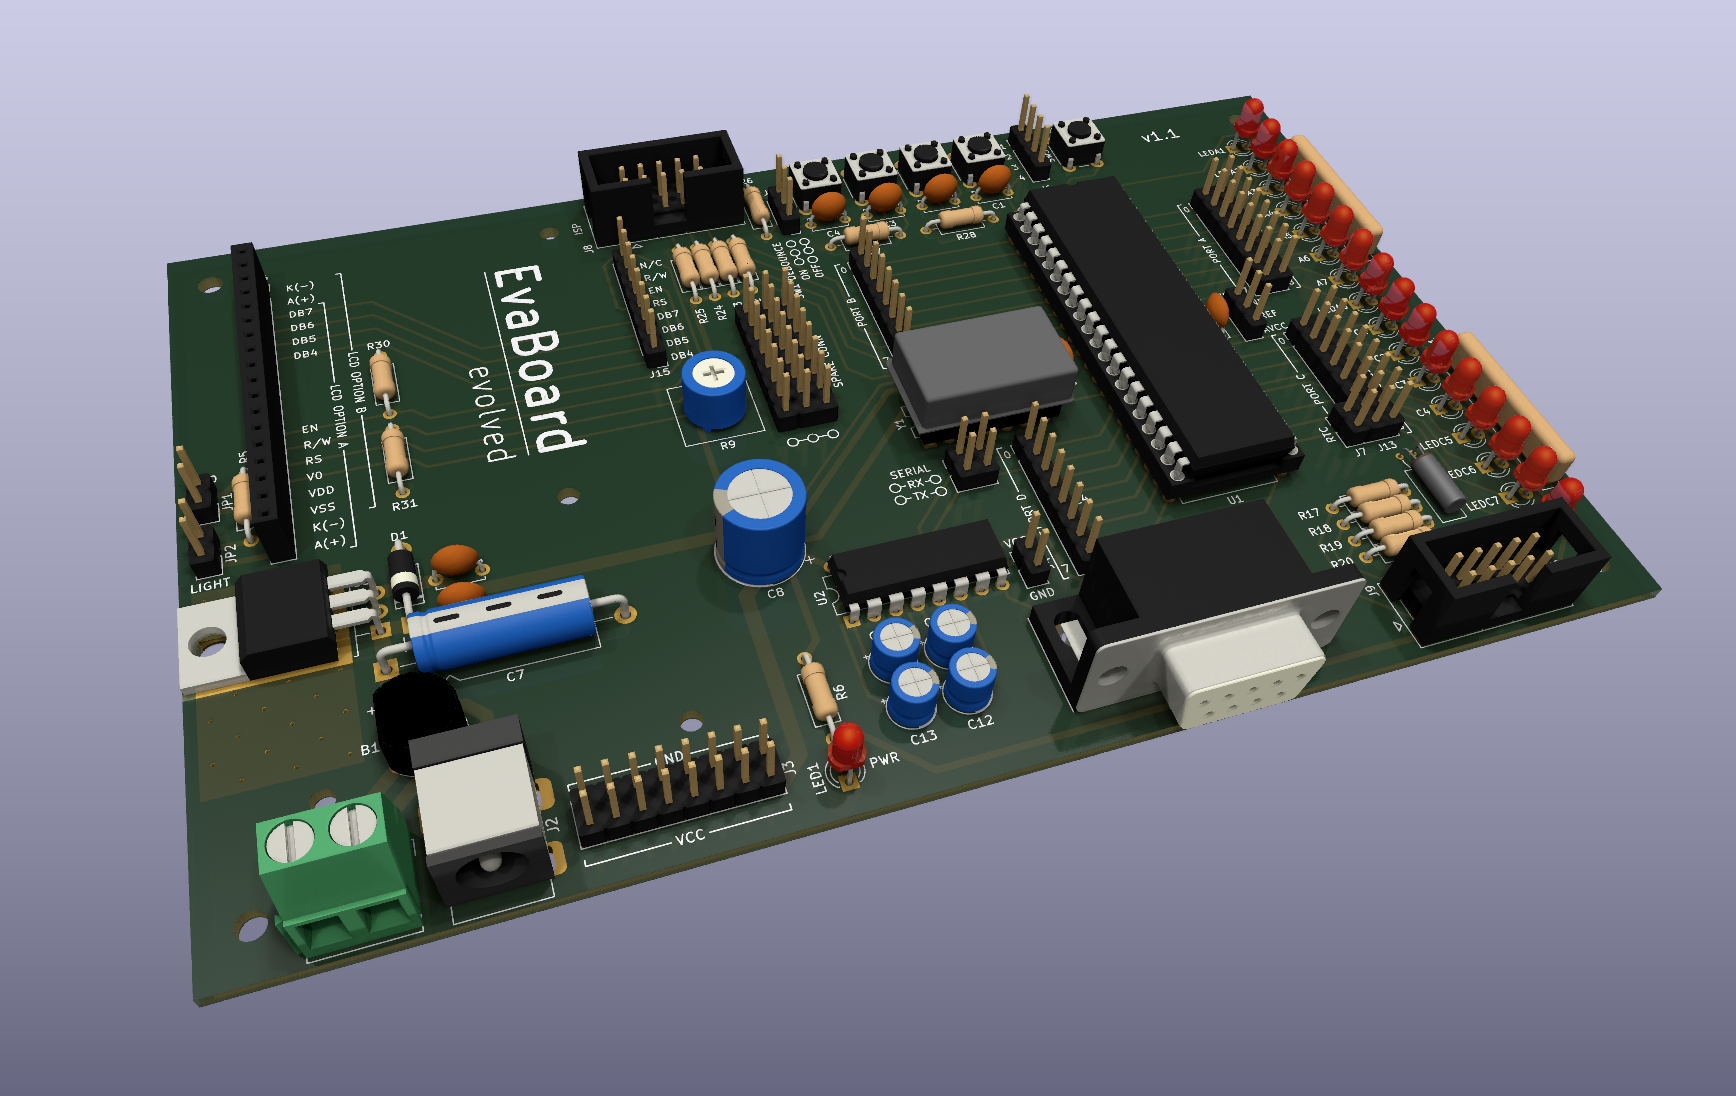
\includegraphics[width=\textwidth]{Pictures/EvaBoard3DRender.png}
\end{titlepage}
\hypersetup{pageanchor=true}

\tableofcontents
\section{Introduction}
This is an evaluation board for the ATmega644(A). It is inspired by (and compatible with) the \href{https://www.embedded.rwth-aachen.de/doku.php?id=lehre:atmegaevaboard}{evaluation board} used in the lab course ``Praktikum Systemprogrammierung'' in the computer science curriculum at RWTH Aachen. 

The university encourages students and educators to build the board themselves. However, the resources it provides are outdated, not well-explained, and at times outright faulty. 

This project provides a complete remake of the original board with a focus on open source software and budget-friendly components. It also includes a ton of documentation, especially for students who have not worked with electronics before. 

There are two add-on boards available in separate repositories:

\begin{itemize}
	\item \href{https://github.com/7vgn/SRAMBoard/}{SRAMBoard} adds an external 128kByte SRAM
	\item \href{https://github.com/7vgn/ADDABoard/}{ADDABoard} for experimenting with analogue-to-digital and digital-to-analogue conversion
\end{itemize}

\subsection{Getting to Know the Evaluation Board}\label{sec:boardOverview}
At the heart of the evalation board is the \emph{ATmega644(A) microcontroller}\footnote{The versions with and without the ``A'' are for all practical purposes the same} from \href{https://www.microchip.com/}{Microchip Technology Inc}. A microcontroller is essentially a CPU with all the necessary peripherals (memory, pin drivers, communication modules etc.) included, which means it needs almost no additional external components to function. Figure \ref{fig:schematicATmega} shows the central part of the board's schematic. 
\begin{figure}[htb]
\centering
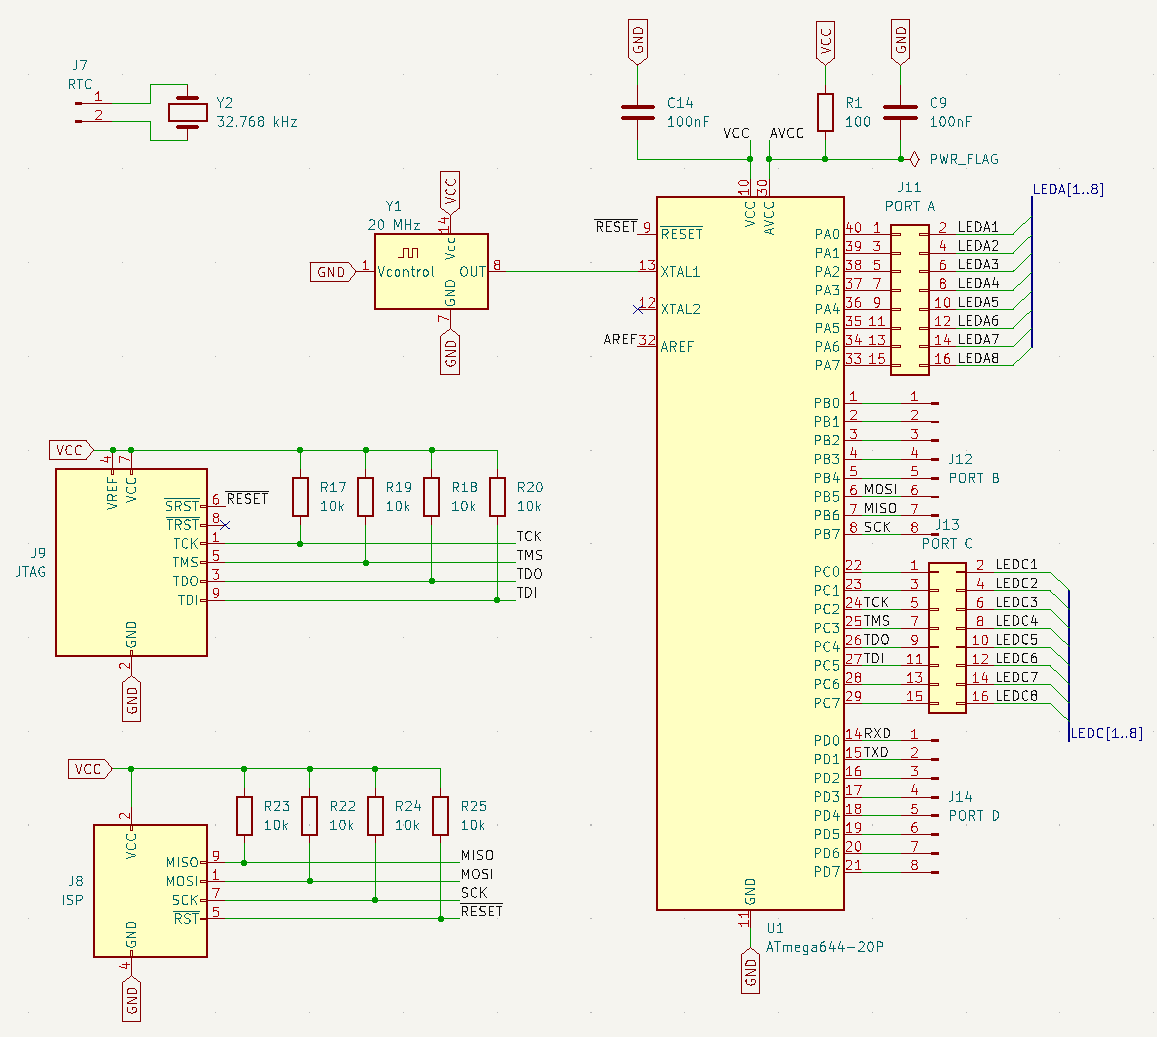
\includegraphics[width=0.85\textwidth]{Pictures/SchematicATmega.png}
\caption{Schematic of the Main Part of the Board}
\label{fig:schematicATmega}
\end{figure}

The one thing it does need is a \emph{supply voltage}, in this case 5V. Most of the components in the lower left quadrant of the board are there to provide just that. Figure \ref{fig:schematicPowerSupply} shows the relevant part of the schematic. A DC power supply can be connected to the board either via the barrel jack J1 or the screw terminal J2. The bridge rectifier B1 ensures that the positive and negative leads are connected to the correct nets, regardless of which way the power is plugged in. The 7805 linear voltage regulator U3 brings the voltage down to a stable 5V. 
\begin{figure}[htb]
\centering
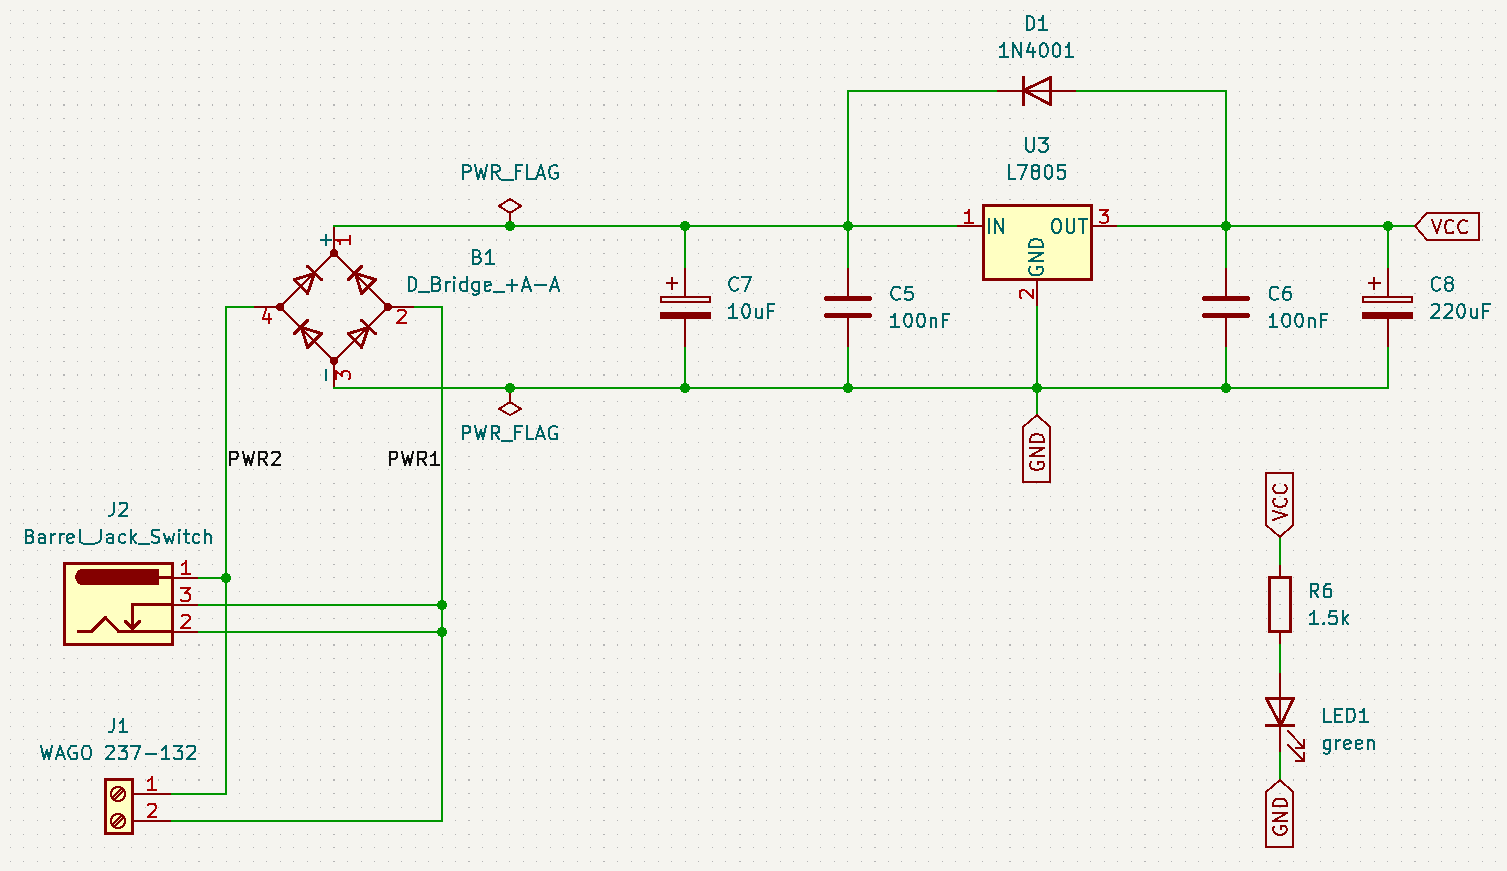
\includegraphics[width=0.85\textwidth]{Pictures/SchematicPowerSupply.png}
\caption{Schematic of the Power Supply Part of the Board}
\label{fig:schematicPowerSupply}
\end{figure}

In order to run, the microcontroller needs a \emph{clock source}, i.e.\ a circuit that outputs a steady stream of alternating high (5V) and low (0V) voltages. While the ATmega644 has an internal oscillator providing an 8MHz clock, higher speeds (up to 20MHz) require an external clock source, in our case the 20MHz crystal oscillator Y1. 
There is a secondary optional watch crystal (Y2) with much lower frequency but higher accuracy that the microcontroller can use for a real time clock. In order to use it, jumper the lower left two pins of J13 (Port C6 and C7) to J7. 

Machine code can be transferred to the microcontroller via one of two interfaces, \emph{ISP} and \emph{JTAG}. There is a pin header for each of them (J8 and J9). These headers are connected to the appropriate pins of the microcontroller, both including the reset pin which suspends the controller's operation during programming. The reset pin is also connected to the \emph{reset button} (SW5), allowing the user to manually hold the microcontroller in reset. The reset line has a pull-up resistor (R25) which keeps the voltage high while no programmer is attached and prevents accidental resets. 

Of the microcontroller's 40 pins, 32 are software-controllable \emph{general purpose inputs/outputs} (GPIO), organised in four groups (Port A, B, C, and D) of 8 pins each (0..7). On the evaluation board, these pins are connected to pin headers (J12, J14 and the left-hand columns of J11 and J13), where the user can attach cables or jumpers to connect them to things. 

Many pins have alternate functions. Check Figure 1-1 in the \datasheet{} for a complete pinout of the ATmega644(A). For example, Pins C6 and C7 can act as TOSC1 and TOSC2, i.e.\ connectors for a secondary oscillator. 

The rest of the board is just there to make working with the microcontroller more comfortable:

\begin{itemize}
\item 16 \emph{LEDs} (LEDA1..8 and LEDC1..8) with their anodes connected to 5V via current-limiting resistors (RN1 and RN2). Their cathodes are connected to the right-hand columns of J11 and J13. When any of those pins gets connected to GND, the corresponding LED lights up. Typically, you would connect them to micrcontroller pins, configure the latter as outputs and then control the LEDs via software. This is particularly easy to do with the Port A and Port C pins as they are located directly adjacent. Be aware that the logic is inverted: an LED is on when its corresponding pin is connected to GND (logic 0), and off when connected to 5V (logic 1). 
\item 4 \emph{buttons} (SW1..4) along the top of the board connect the respective pin on J6 to ground while pressed. If you wire any of these to some microcontroller pin and configure the pin as input, you can read the state of the button from software (again with inverted logic). You must activate the internal pull-up resistor for the pin, otherwise you won't get a logic 1 when the button is not pressed. \\
Each button has a rudimentary \href{https://en.wikipedia.org/wiki/Switch\#Contact\_bounce}{debouncing} circuit to avoid spurious inputs. For SW1, this can be disabled via JP3. See Figure \ref{fig:schematicLEDsButtons} for details. 
\begin{figure}[htb]
\centering
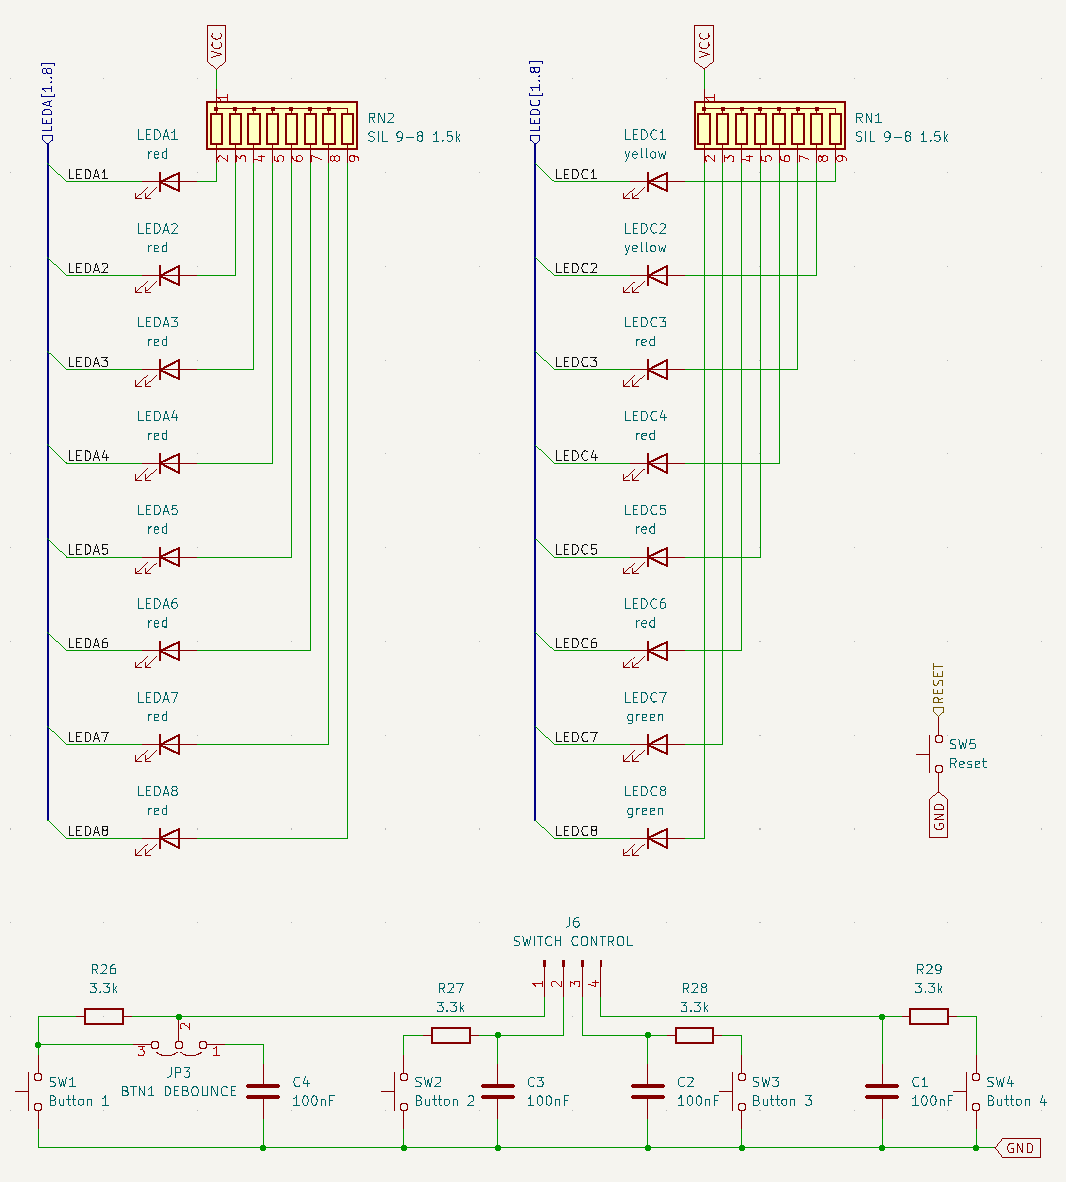
\includegraphics[width=0.85\textwidth]{Pictures/SchematicLEDsButtons.png}
\caption{Schematic of the LEDs and Buttons}
\label{fig:schematicLEDsButtons}
\end{figure}
\item An HD44780-compatible\footnote{The HD44780 was a driver IC for dot matrix LCDs by Hitachi. While it is now dicontinued, many clones exist and it has become a quasi-standard for these kinds of LCDs.} \emph{LCD} module can be plugged into J16. These types of LCD need a supply voltage (via JP1), a voltage for their LED backlight (via R5 and JP2), and a third voltage to set the contrast (adjustable via R9). Seven signal lines (RS, EN, R/W, and DB4..7) are used to communicate with the LCD and these are routed to J15 from where they can be wired to some microcontroller pins. See Figure \ref{fig:schematicLCD}. Since communicating with these LCDs is a bit complicated, a \href{../Drivers/LCD/}{driver} is available in this repository. 
Most HD44780-compatible LCD modules come with one of two standard pin layouts. This board can accomodate both kinds. For more details, see Section \ref{sec:compOptional}. 
\begin{figure}[htb]
\centering
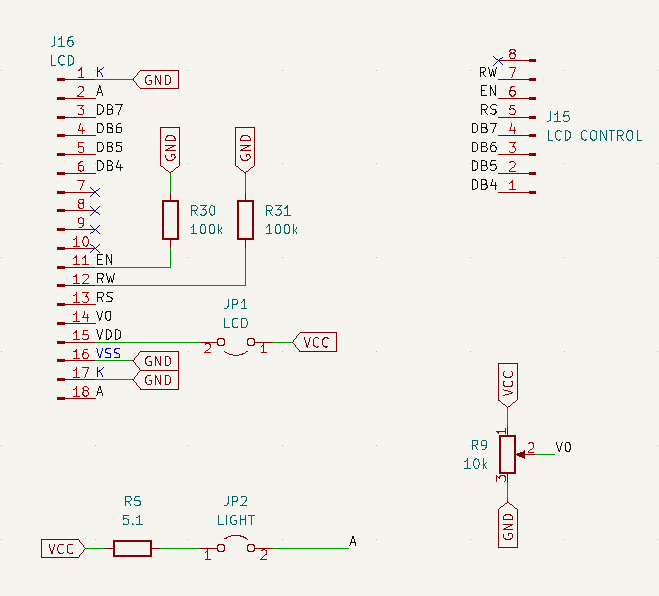
\includegraphics[width=0.85\textwidth]{Pictures/SchematicLCD.png}
\caption{Schematic of the LCD circuitry}
\label{fig:schematicLCD}
\end{figure}
\item Finally, the board provides a \emph{serial} connector (J10) which can be used for different purposes. The most common one is to connect it to a computer to send text messages back and forth. A MAX232 driver IC converts between the microcontroller's voltage levels (0V and 5V) and those required by \href{https://en.wikipedia.org/wiki/RS-232}{RS-232} (-15V..-3V and +3V..+15V). It uses a \href{https://en.wikipedia.org/wiki/Charge\_pump}{charge pump} involving C10..C13 to generate +9V and -9V from the 5V supply voltage. The ATmega has two pins, RX (Pin D0) and TX (Pin D1) which can be dedicated to serial communication. To connect these to the MAX232, mount jumpers on JP4, see Figure \ref{fig:schematicSerial}. Don't forget to dismount the jumpers before using these pins as GPIOs!
\begin{figure}[htb]
\centering
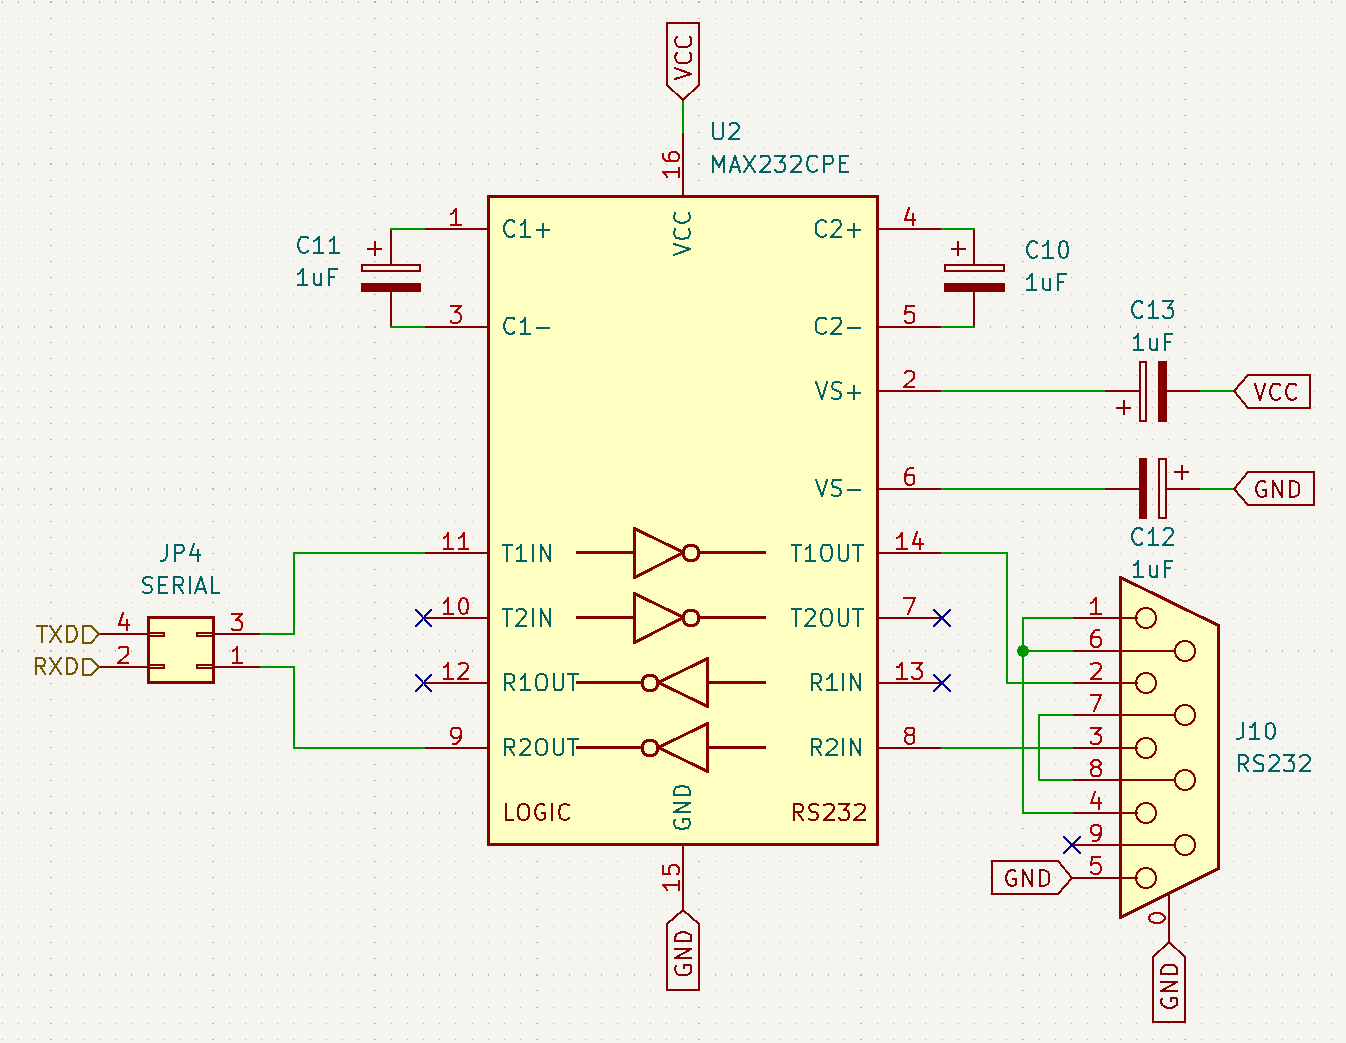
\includegraphics[width=0.85\textwidth]{Pictures/SchematicSerial.png}
\caption{Schematic of the Serial Communication Part of the Board}
\label{fig:schematicSerial}
\end{figure}
\end{itemize}

Figure \ref{fig:topView} gives an idea of the board's layout. For more details, have a look at the board's complete \href{../KiCAD/Pictures/Schematic.pdf}{schematic}. 
\begin{figure}[htb]
\centering
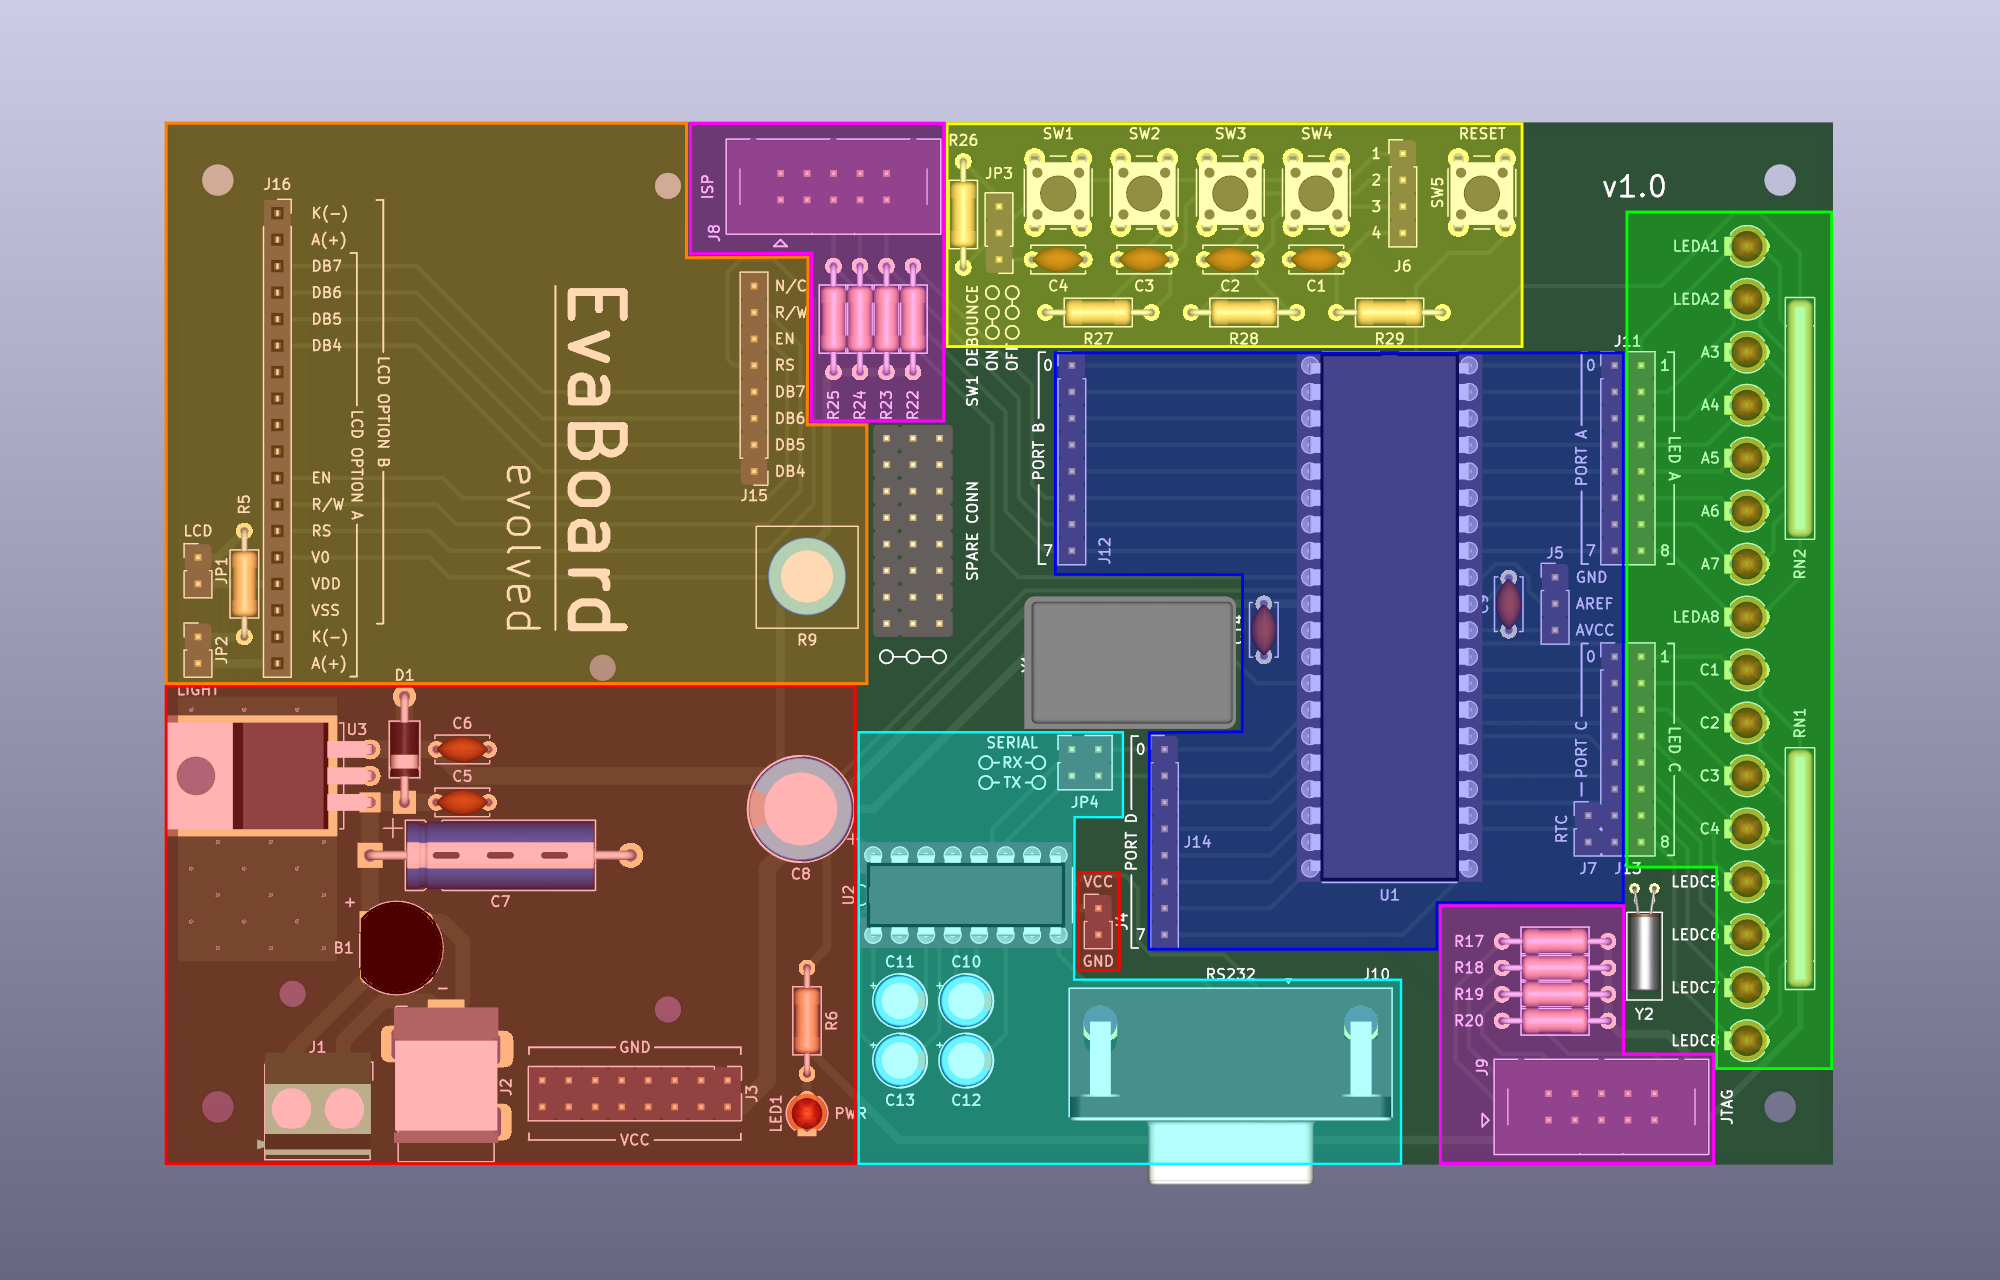
\includegraphics[width=0.85\textwidth]{Pictures/TopView.png}
\caption{Layout of the board: Microcontroller and GPIO headers (blue), Programming (purple), Power Supply (red), LEDs (green), Buttons (yellow), Serial (mint), LCD (orange)}
\label{fig:topView}
\end{figure}

\subsection{Changes from the Original Board}\label{sec:differences}
While the board was designed to be as similar as possible to the original, there are some notable changes. Some fix issues while others provide more options for the components. Most importantly, the position of the pin headers has not changed which means you can use add-on boards from the original board and vice versa. Here is a list of all the changes:

\begin{itemize}
\item There were two pull-up resistors on the reset line, making it effectively 5kΩ. While that would probably still work, some programmers might have a hard time. 
\item The power plug was seriously messed up. The intended model was a very specific and hard to get one (Lumberg 1613 18) which the BOM didn't even list correctly. This barrel jack needed a rectangular hole in the PCB which almost completely cut a trace.\\
In the remade version, the trace was moved. It is still possible to use the same barrel jack, but now more common (and cheaper) ones fit, too. 
\item The originally intended LCD is unreasonable expensive (approximately 14\euro{}, when you can get similar ones for less than 5\euro{}). It also has a very uncommon pin layout, making it difficult to find affordable alternatives.\\
The remade board offers two options, allowing for both the original LCD as well as ones with the standard pin layout. The only downside to the latter is that they stick out over the side of the board and only one of the four mounting screws can be used. That is usually not a problem, it should hold even without any screws. 
\item The unused eighth pin of J15 used to be GND. This is needlessly dangerous when the LCD is connected to a port via an 8-pole cable. If the eighth pin of the microcontroller is accidentally configured as a high output, it gets shorted to GND. In the remade version, the eighth pin is not connected. 
\item The crystal oscillator was moved slightly upwards to make the serial jumpers more easily accessible. 
\item Pin 2 of the MAX232 was connected via C13 to GND instead of VCC. While some manufacturers allow this (TI for example, see footnote to Figure 6 in the \href{https://www.ti.com/lit/ds/symlink/max232.pdf}{datasheet}), others (like Maxim, see Figure 5 in the \href{https://www.analog.com/media/en/technical-documentation/data-sheets/max220-max249.pdf}{datasheet}) do not and we've seen parts go up in smoke due to this. The remade board has it connected to VCC instead which works for all MAX232. 
\item Added D1 to protect U3 in case the board is supplied with power directly via its VCC net (as is the case with the original AD/DA add-on board). 
\item The original board made a half-hearted attempt at debouncing the buttons by adding capacitors in parallel. While this works to some extend when releasing a button, it causes a brief but very large current when pressing it. The new board adds R26..R29 to avoid that. This required a change to the jumper (JP3) that controls the debouncing of SW1. It is now a three-pin (two-position) jumper instead of a 2-pin (on-off) one. The solution is still not ideal and relies on the (very small) hysteresis of the ATmega's inputs. Fortunately, the buttons are not very bouncy to begin with. 
\item Added a 24-pin header ("SPARE CONN") to allow three-way connections or just as a storage space for spare jumpers. 
\end{itemize}

\begin{caution}
The university hands out an LCD driver to students which has a serious flaw: While querying the LCD's busy flag, it briefly configures both the LCD's and the microcontroller's data pins as outputs, causing a short. This lasts only for one clock cycle but that is enough to sometimes cause damage to an LCD. 

For safety, it is highly recommended to use the \href{../Drivers/LCD/}{LCD driver} provided in this project instead.
\end{caution}

\section{Building the Board}
\subsection{Necessary Parts and Tools}
\subsubsection{Tools}\label{sec:tools}
As a bare minimum, you need a soldering iron, solder, some pliers, and wire cutters, see Figure \ref{fig:solderingTools}.  Find a workspace with a fireproof surface, make sure it is well-lit and well-ventilated. Keep soldering materials away from any kind of food, small children, and pets. 
\begin{figure}[htb]
\centering
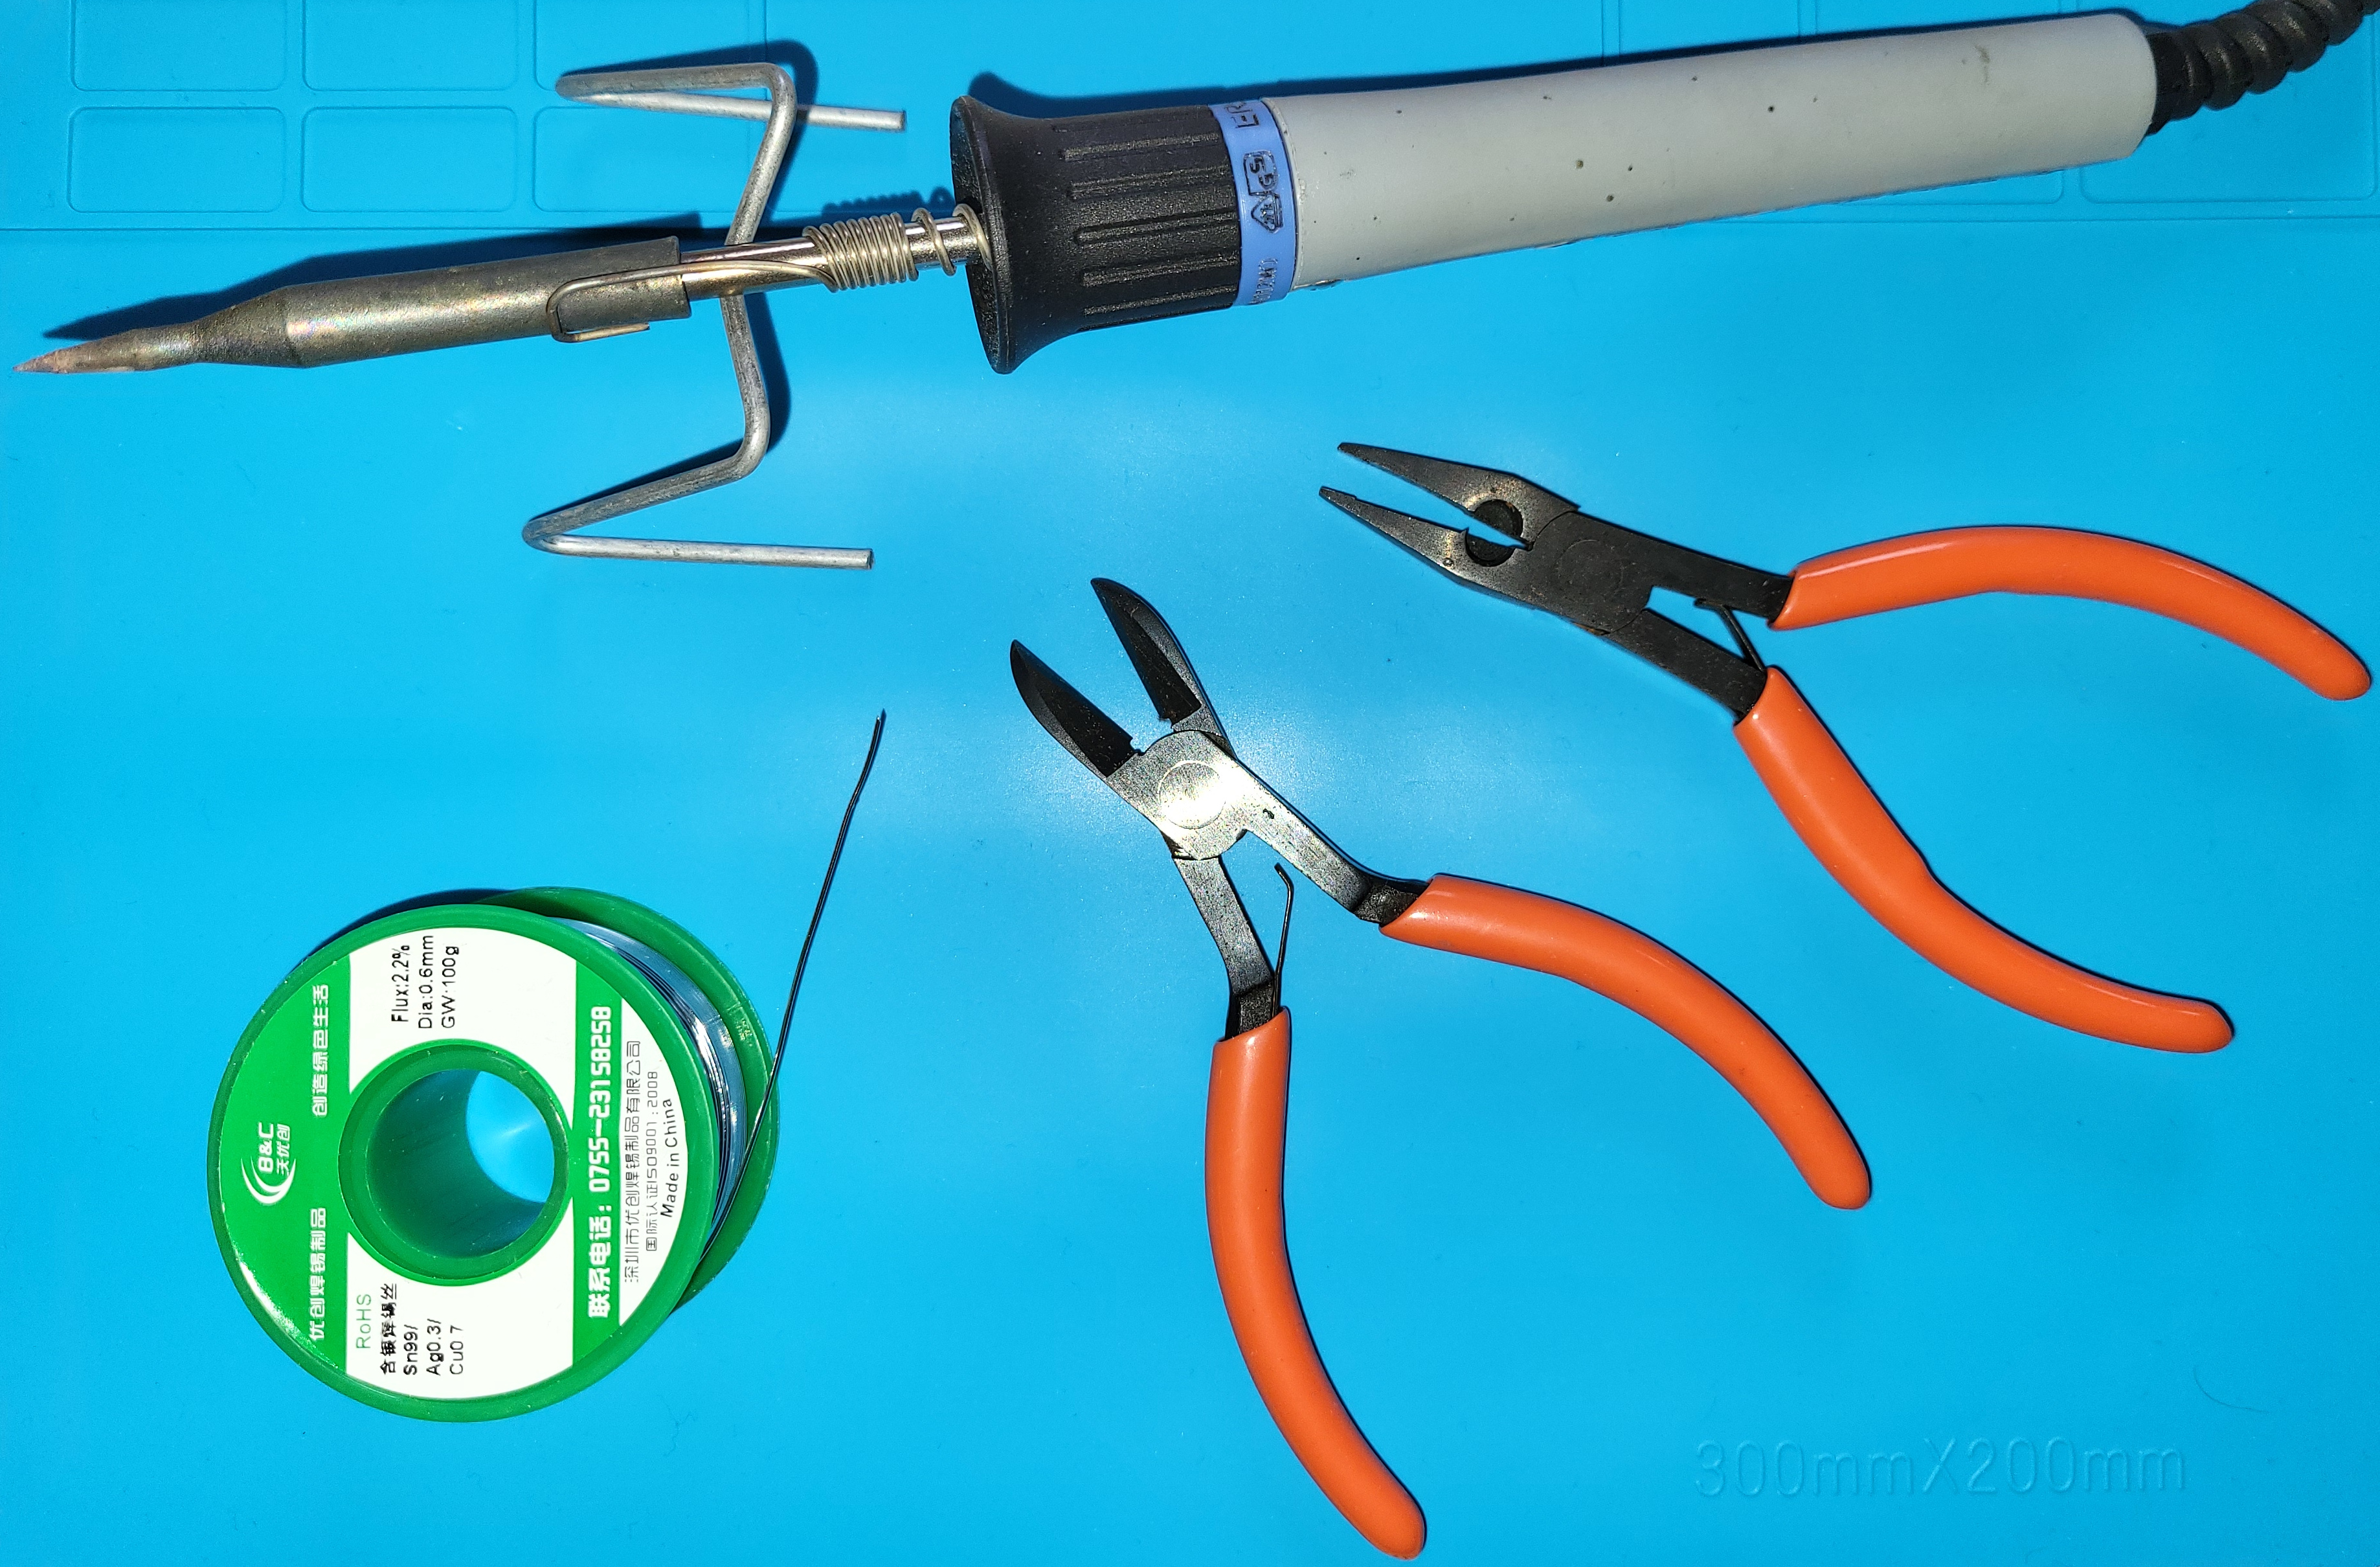
\includegraphics[width=0.85\textwidth]{Pictures/Tools.jpg}
\caption{Basic Tools for Soldering the Board}
\label{fig:solderingTools}
\end{figure}

For the soldering iron, as a rule of thumb, smaller is better when it comes to electronics. But since all components are relatively large, most common soldering irons will work. The solder should not be too thick (something like 1mm diameter works great) and contain a flux core. Leaded solder is slightly easier to work with but poses a health risk. It is highly recommended to use lead-free solder. 

If you need to undo a solder joint, you can use a solder pump and/or some solder wick. But any de-soldering carries the risk of damaging components or the PCB. It is much better to avoid it in the first place. 

The board needs a DC voltage between 7.5V and 12V. Theoretically, up to 25V are possible but since the voltage regulator U3 turns the surplus into heat, it is not recommended to go that high. You don't need an expensive bench supply. A standard wall plug (10..15\euro) with up to 1A output current should be more than enough to power your board. Some like the one in Figure \ref{fig:wallPlug} have an adjustable voltage so they can be used for other things, too. 
\begin{figure}[htb]
\centering
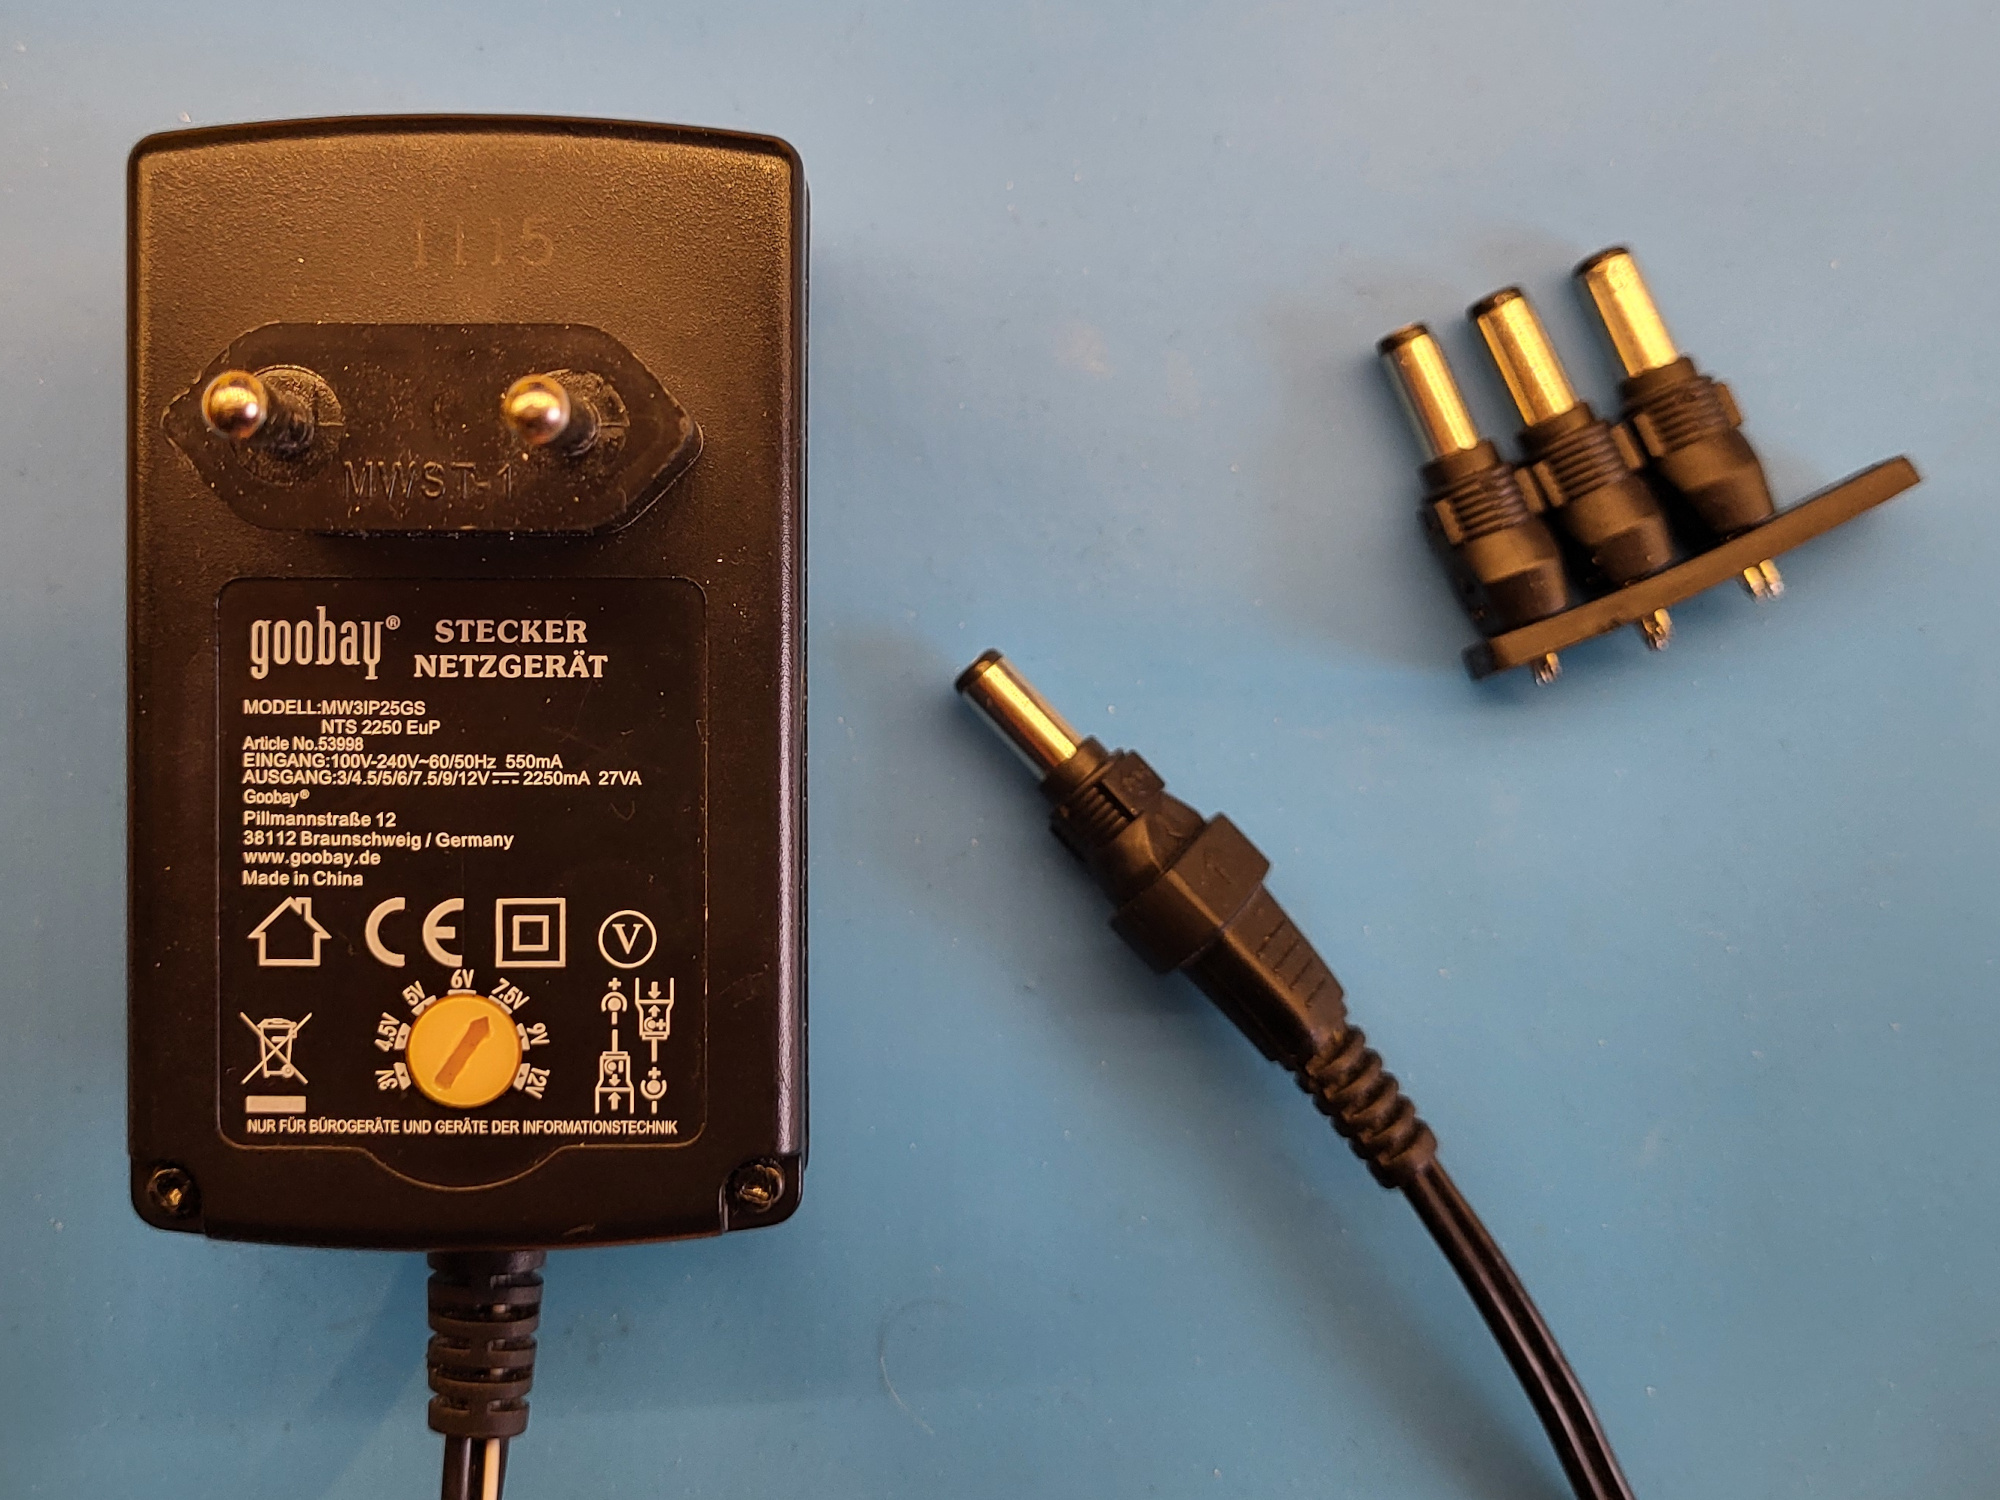
\includegraphics[width=0.85\textwidth]{Pictures/WallPlug.jpg}
\caption{Wall plug as power supply. This one comes with interchangeable plugs.}
\label{fig:wallPlug}
\end{figure}

If you have a phone charger that supports USB Power Delivery (USB PD) at 9V or 12V, you can also use that. In order to get the charger to actually output 9V or 12V rather than the default 5V, you need a ``trigger cable'' (sometimes called ``decoy cable''). These cables contain a chip that negociates the higher voltage with the charger. They can be bought for cheap (3..8\euro) and some even come with a power jack that fits into the J2 connector. 

In order to copy machine code from your computer to the microcontroller, you need a programmer. ISP programmers come as cheap as 5\euro . See Section \ref{sec:programmers} for details. 

Optional: When debugging programs on the microcontroller, it can be handy to have a serial connection to send debug messages to the computer. The board has a 9-pin D-subminiature connector (J10). If your computer still has a serial port, you only need a serial cable. Otherwise, you can buy a USB to serial converter. See Figure \ref{fig:serialOptions}. 
\begin{figure}[htb]
\centering
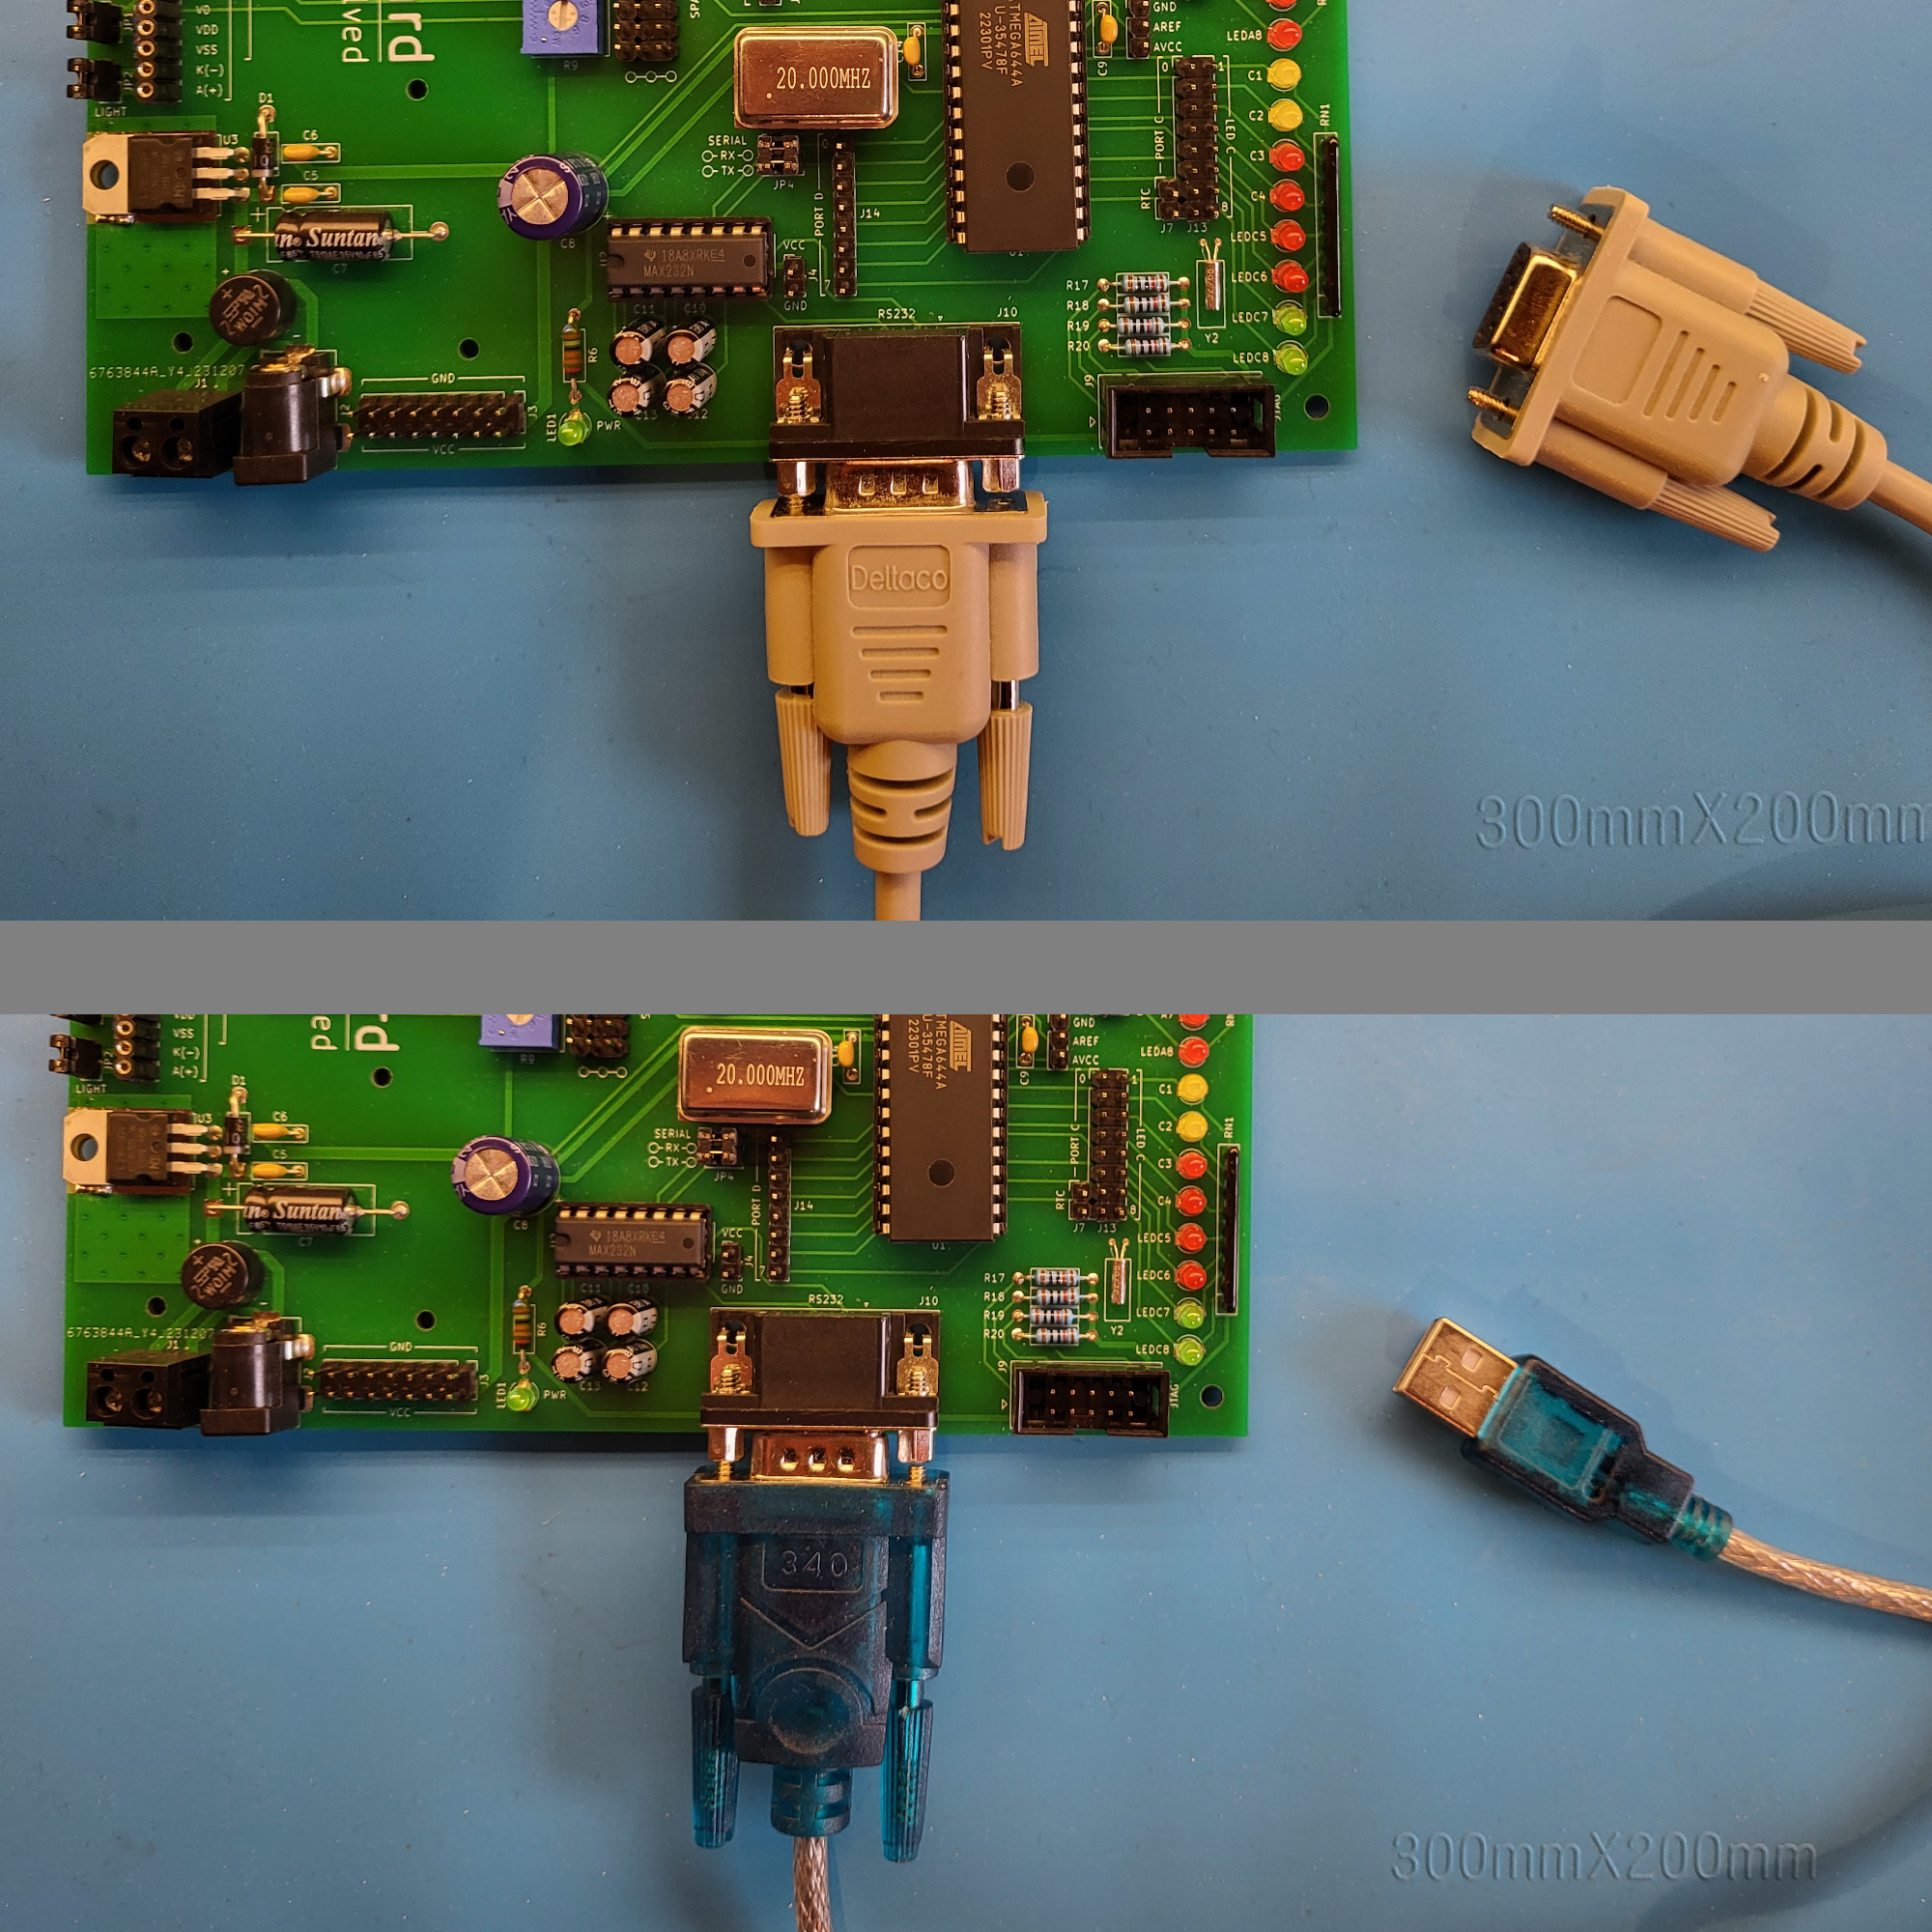
\includegraphics[width=0.85\textwidth]{Pictures/SerialOptions.jpg}
\caption{Options for Serial Connection}
\label{fig:serialOptions}
\end{figure}

Optional: A multimeter (even a cheap one like in Figure \ref{fig:multimeter}) is a great help for testing or debugging your solder work. 
\begin{figure}[htb]
\centering
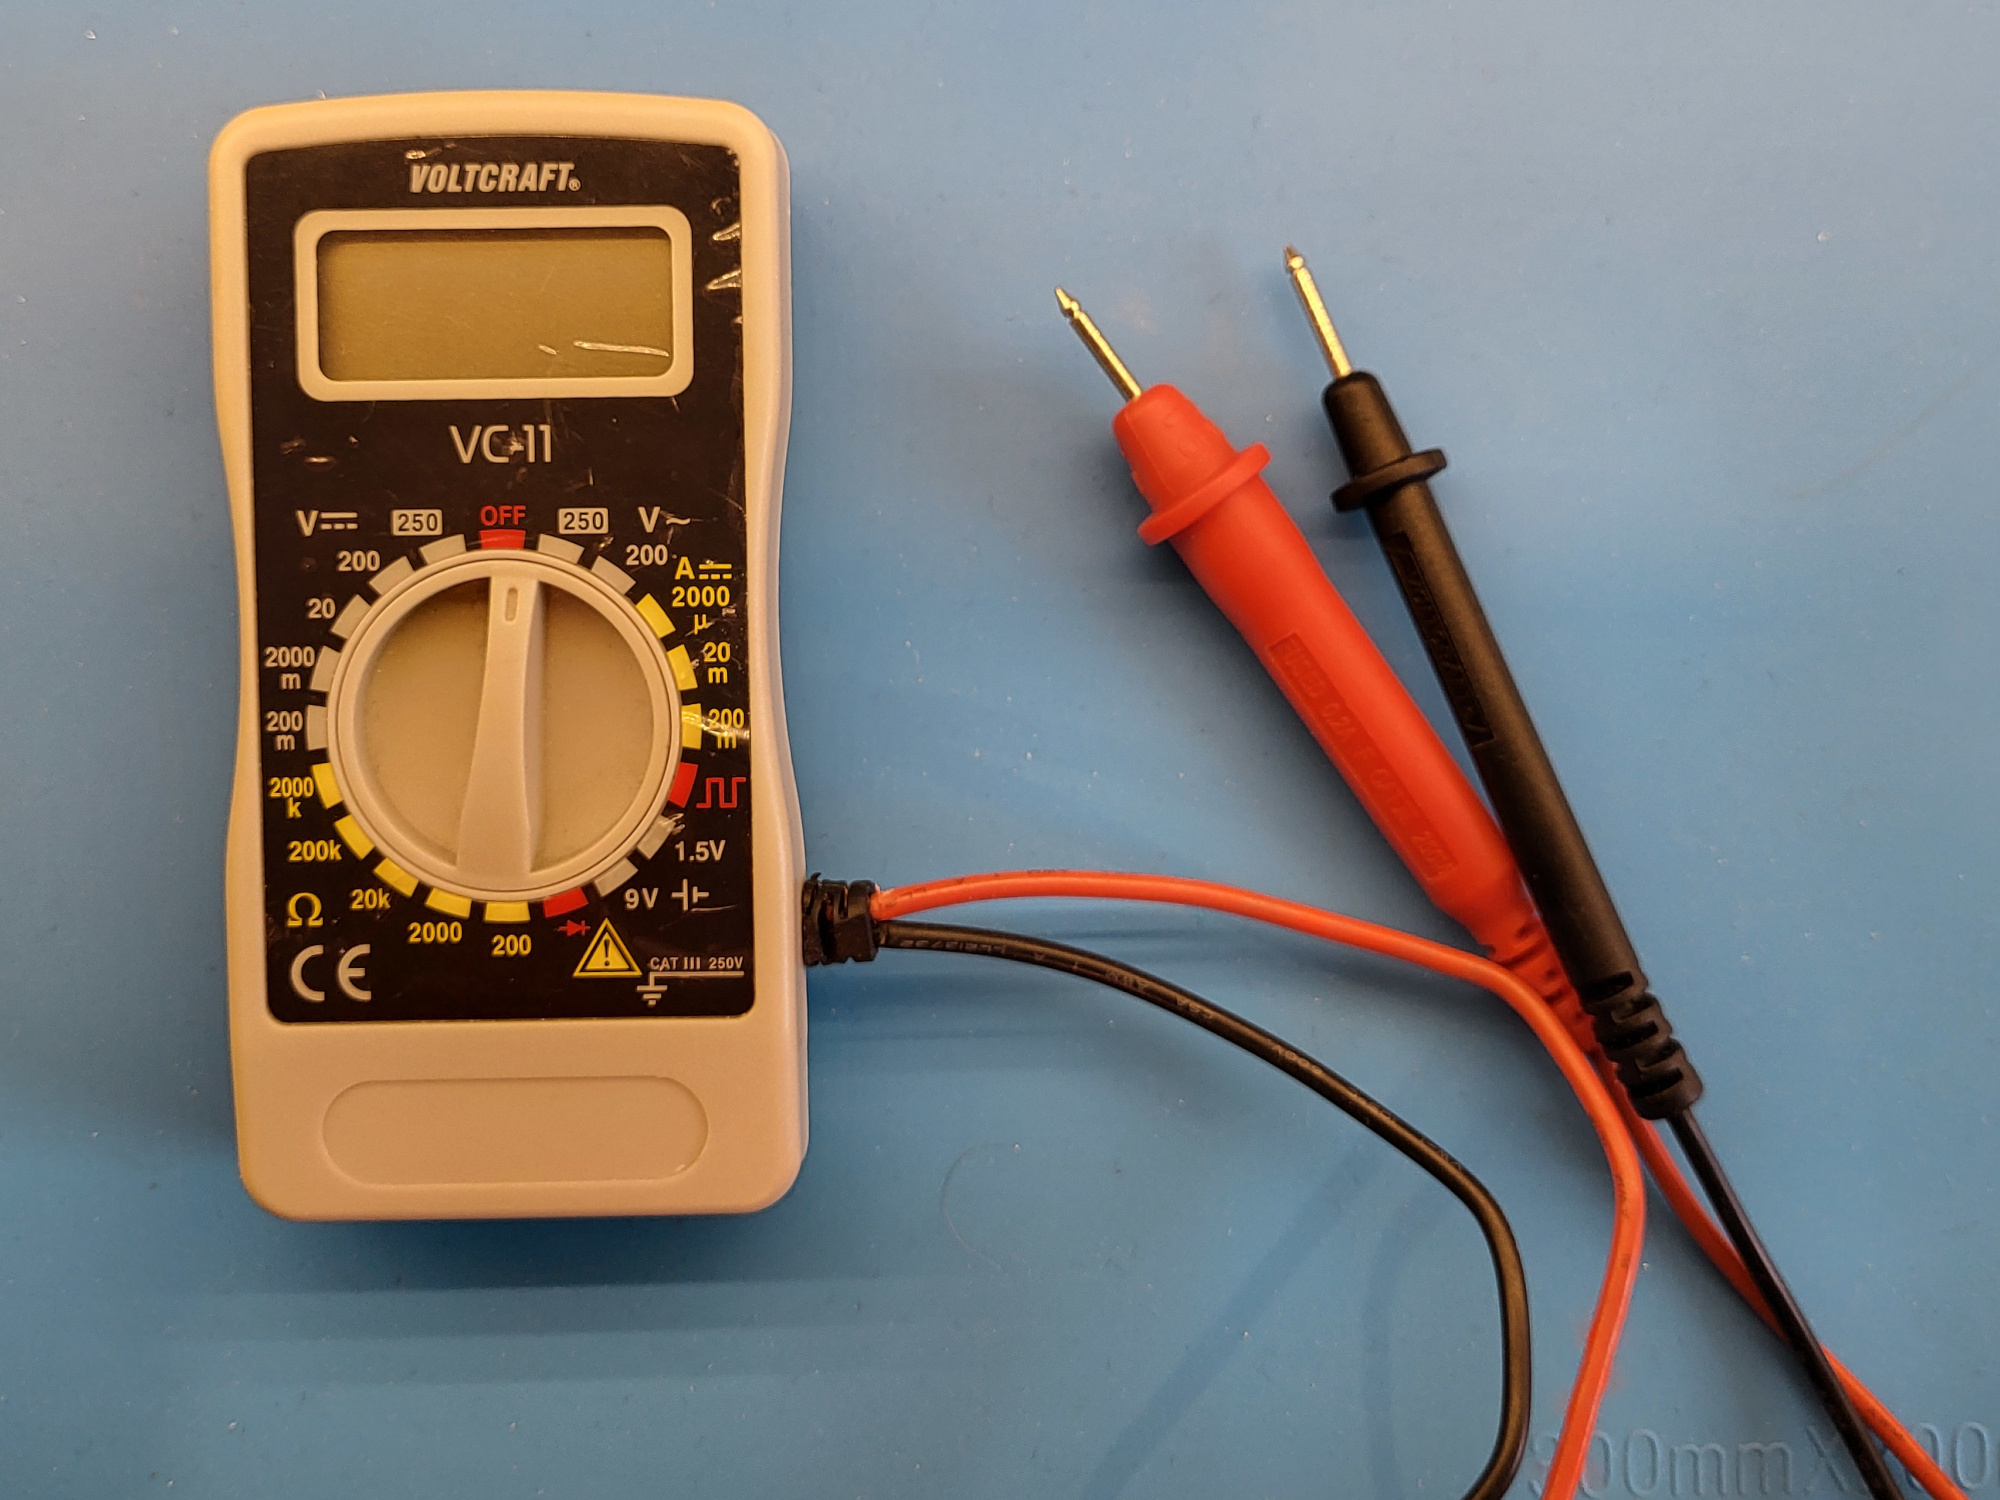
\includegraphics[width=0.85\textwidth]{Pictures/Multimeter.jpg}
\caption{Even the cheapest multimeter will do. This one was literally free.}
\label{fig:multimeter}
\end{figure}

\subsubsection{Getting the PCB}\label{sec:pcb}
The PCB (printed circuit board) is the base of the board. It holds all the components and makes the electrical connections between them via copper traces on the top and bottom side (it's a ``2-layer board''). It was designed using the open source software \href{https://www.kicad.org/}{KiCAD}. 

While it is possible to make PCBs yourself, it is definitely not recommended for beginners. There are a number of PCB manufacturers that produce self-designed PCBs in small quantities for hobbyists. The cost of PCB manufacturing has gone down massively in recent years but since most of the affordable ones ship from China, expect a delay of roughly two weeks. 

The cost for the PCB itself is usually dwarfed by the shipping cost. That's why you will typically get five or more PCBs for the same total price as a single one. If you find other students who want to build the board as well, you might get away with less than 5\euro{} per PCB. Consider including PCBs for the add-on boards in the same order. 

Some manufacturers accept a KiCAD project, but most will want so-called ``gerber files''. To create those, install KiCAD (the board was designed with version 6, but newer ones probably work, too). For Windows, there is an \href{https://www.kicad.org/download/windows/}{installer}. On Linux, you can use a package manager to install the packages \texttt{kicad} and \texttt{kicad-packages3d}. 
Start KiCAD and open the project from the \href{../KiCAD/}{\file{KiCAD/} subdirectory} of this repository. Go to the PCB Editor and in the ``File'' menu choose ``Fabrication Outputs'', ``Gerbers''. Enter ``Gerbers/'' for the output directory. Now you need to consult the manufacturer's website for the exact options. These are different for every manufacturer but usually easy to find. Hit ``Plot'' to create the first batch of files. Then click ``Generate Drill Files'' and again follow the manufacturer's guidelines to create drill files. All the gerber files are placed in the \texttt{Gerbers} subdirectory of the KiCAD project. Pack them all into a zip file. This is what you upload on the manufacturer's website. Before you do that, you can check them in KiCAD's own Gerber Viewer from the KiCAD main window. 

During the ordering process, you might be able to choose between different options for the soldermask (the green stuff, but other colors are available) and the surface finish (pre-applied solder on the exposed copper pads). It is highly recommended to get a lead-free finish, even if that costs a little extra. With the leaded option, your board qualifies as toxic waste and you cannot dispose of it in the household rubbish bin. Also lead can cause brain damage. 

\subsubsection{Purchasing Components}\label{sec:comp}
The components you need for the board are listed in the \href{../BOM/BOM.pdf}{bill of materials} (``BOM''). The fastest option is to buy them from a local distributor. In Germany, \href{https://www.reichelt.de/}{Reichelt}, \href{https://www.conrad.de/}{Conrad}, or \href{https://www.pollin.de/}{Pollin} are popular stores. Internationally, \href{https://mouser.com}{Mouser} or \href{https://www.farnell.com/}{Farnell} are well-known. Some of them are more geared towards hobbyist, others target businesses. Pay attention to shipping costs, minimum order value, and whether VAT is included in their listed prices. The BOM lists order codes for Reichelt, but don't read that as an endorsement for that particular distributor. 

Keep an eye out for bulk pricing. Some components like resistors have massive discounts above a certain quantity. If you need 8, check if 10 are cheaper, if you need 40, check 100 etc. 

In order to save on shipping costs, it is probably best to order from as few places as possible. Some of the more expensive components like the microcontroller or the LCD might be cheaper when sourced separately. If you're feeling adventurous, you can try eBay or AliExpress. However, with less reputable sources, there is a risk of getting conterfeit or stolen components. Keep in mind that shipping times from China can be anywhere between one week and infinity. 

Some optional components are not listed in the BOM. For instance, you might want put some feet under the board, using glue or screws (the PCB has 3mm holes for that purpose). 

\subsubsection{Checklist}
\begin{itemize}
\item[\CheckBox{}] PCB (see Section \ref{sec:pcb})
\item[\CheckBox{}] Components from \href{../BOM/BOM.pdf}{BOM} (see also Section \ref{sec:comp})
\item[\CheckBox{}] Tools for soldering: soldering iron, solder, pliers, wire cutters (see Section \ref{sec:tools})
\item[\CheckBox{}] Some kind of power supply (see Section \ref{sec:tools})
\item[\CheckBox{}] Programmer or debugger, including the necessary cables (see Section \ref{sec:programmers})
\end{itemize}

\paragraph{Optional}
\begin{itemize}
\item[\CheckBox{}] Serial cable or USB-to-serial converter
\item[\CheckBox{}] Multimeter
\item[\CheckBox{}] Feet for the board (M2.5)
\item[\CheckBox{}] Screws (M2x18), nuts, washers, and spacers (10mm) for the LCD
\end{itemize}

\subsection{Soldering}
Take your time and go slow and methodically. Familiarise yourself with the board first (see Section \ref{sec:boardOverview}). Have the schematic and BOM at hand so you can refer to them for component numbers and values. 

Start with the resistors. These are the easiest components to solder and they're reasonably resistant to overheating. Make sure you choose a resistor with the correct resistance value (see BOM). For simple resistors (not resistor networks), the orientation doesn't matter. 

Slot a resistor in from the front and bend the wires approximately 45° on the back, so it won't fall out. Turn the PCB around and solder it in from the back. Place the tip of your soldering iron so that it touches both the wire and the pad, then add some solder. The solder should adhere to both parts - if it doesn't, you either haven't heated both parts properly or you're missing flux. Don't use too mush solder: the ideal solder joint is tent-shaped, not a big blob. Don't worry if it doesn't come out perfect right away. Soldering is mainly a matter of practice. You can rework your first joints later once you've got a bit more experience. See Figures \ref{fig:solder1}, \ref{fig:solder2}, \ref{fig:solder3}, and \ref{fig:solder4} for illustration. 
\begin{figure}[htb]
\centering
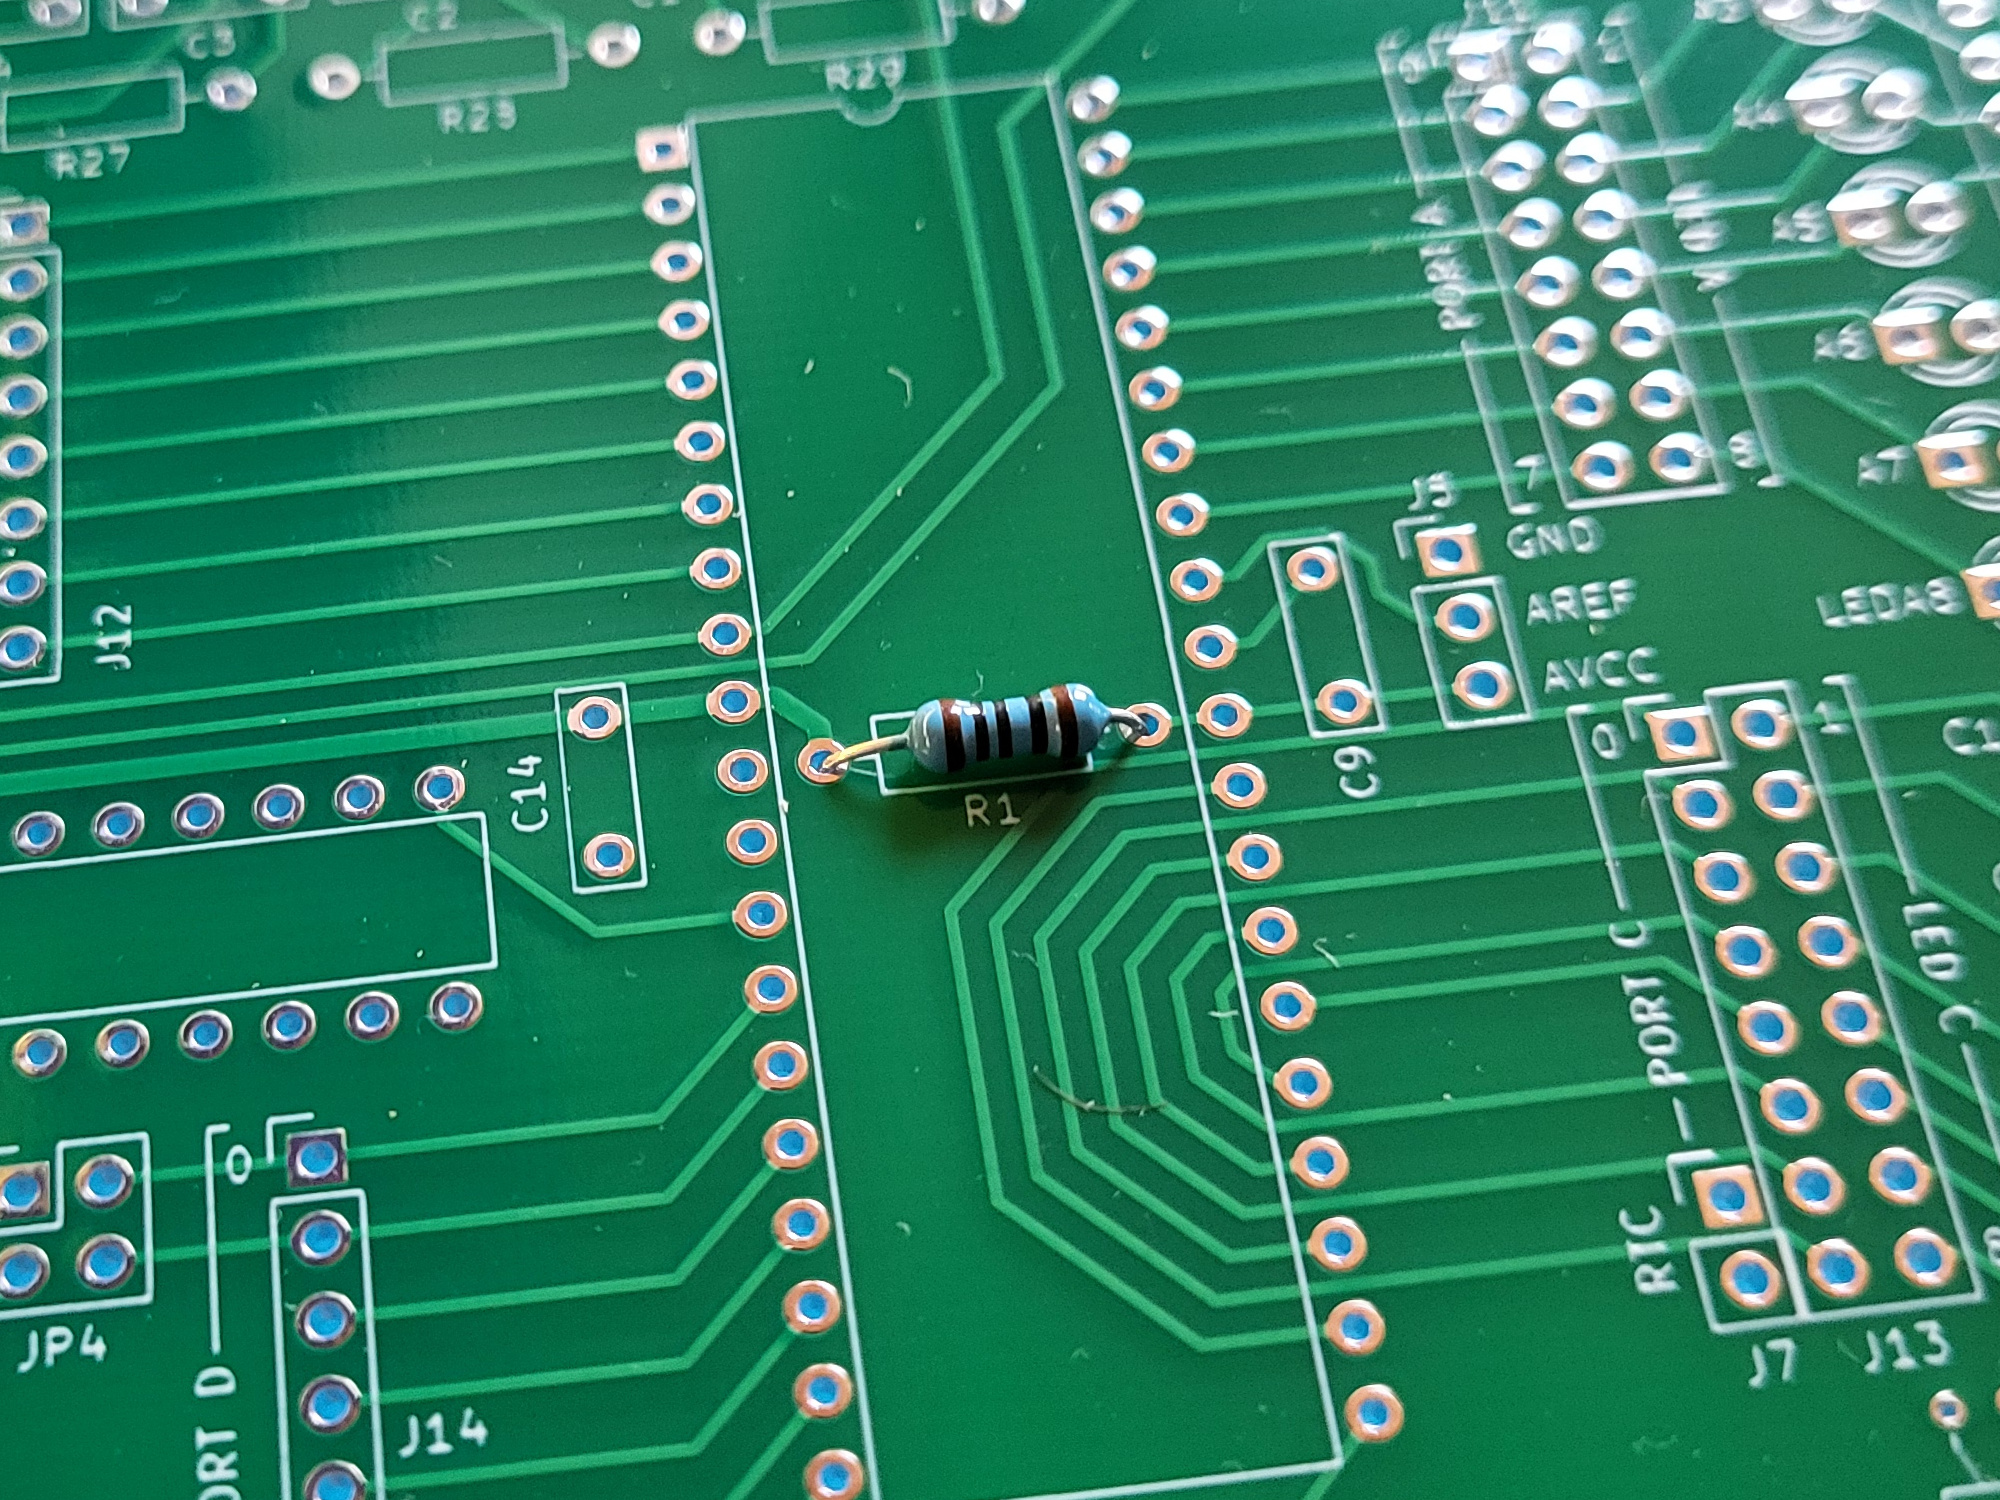
\includegraphics[width=0.85\textwidth]{Pictures/Solder1.jpg}
\caption{Step 1: Insert a resistor into the PCB}
\label{fig:solder1}
\end{figure}
\begin{figure}[htb]
\centering
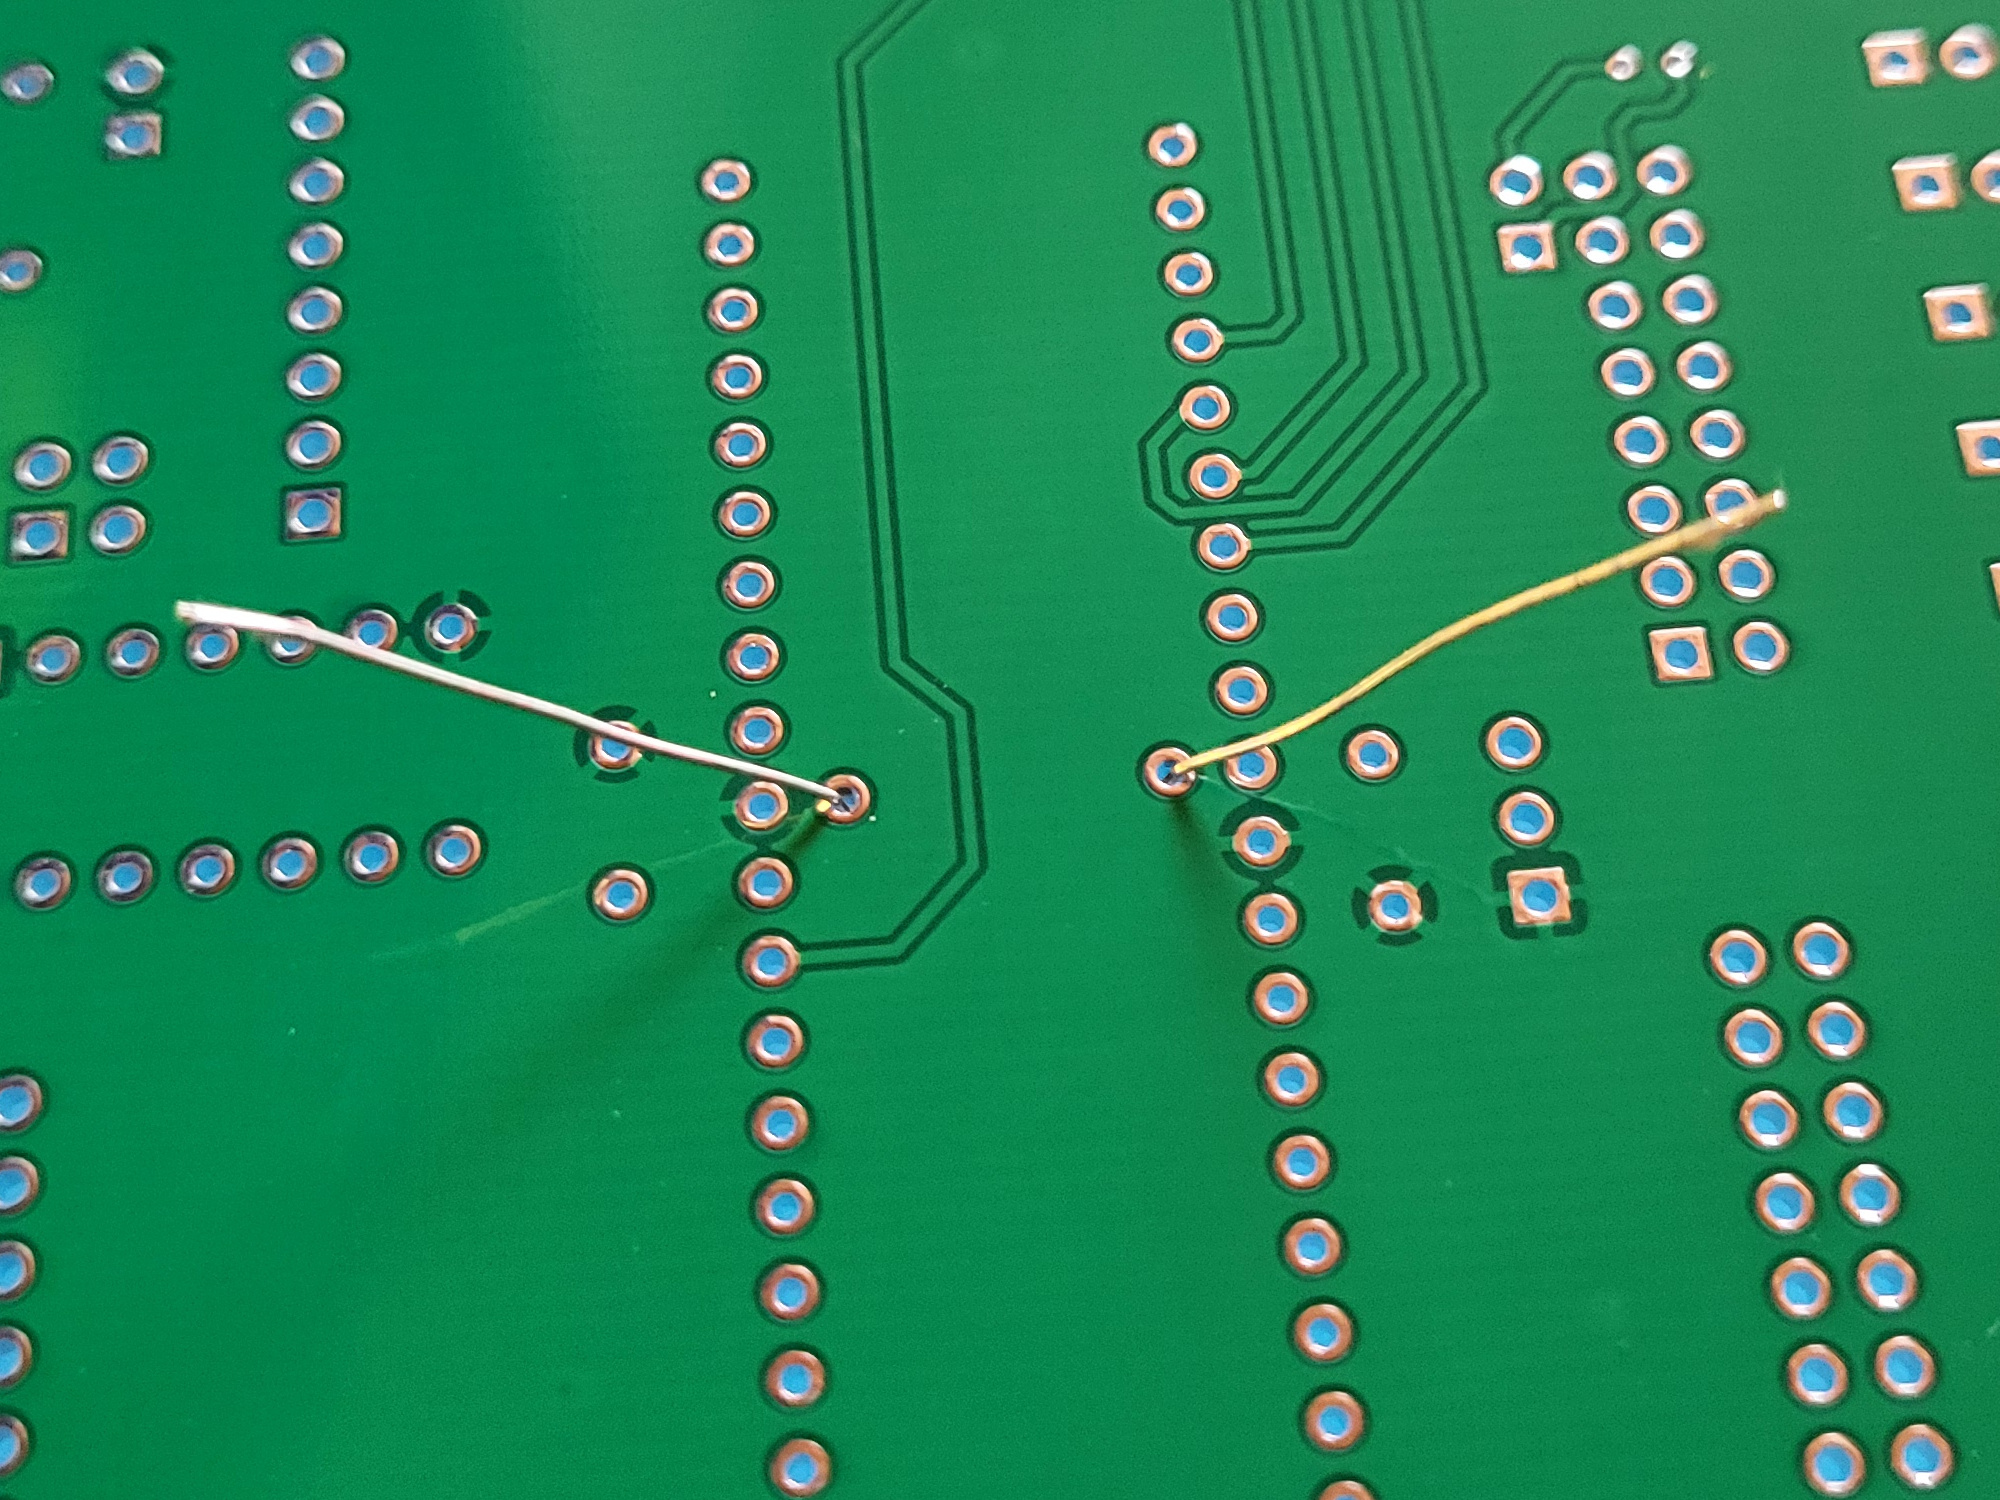
\includegraphics[width=0.85\textwidth]{Pictures/Solder2.jpg}
\caption{Step 2: Bend the wires so it can't fall out}
\label{fig:solder2}
\end{figure}
\begin{figure}[htb]
\centering
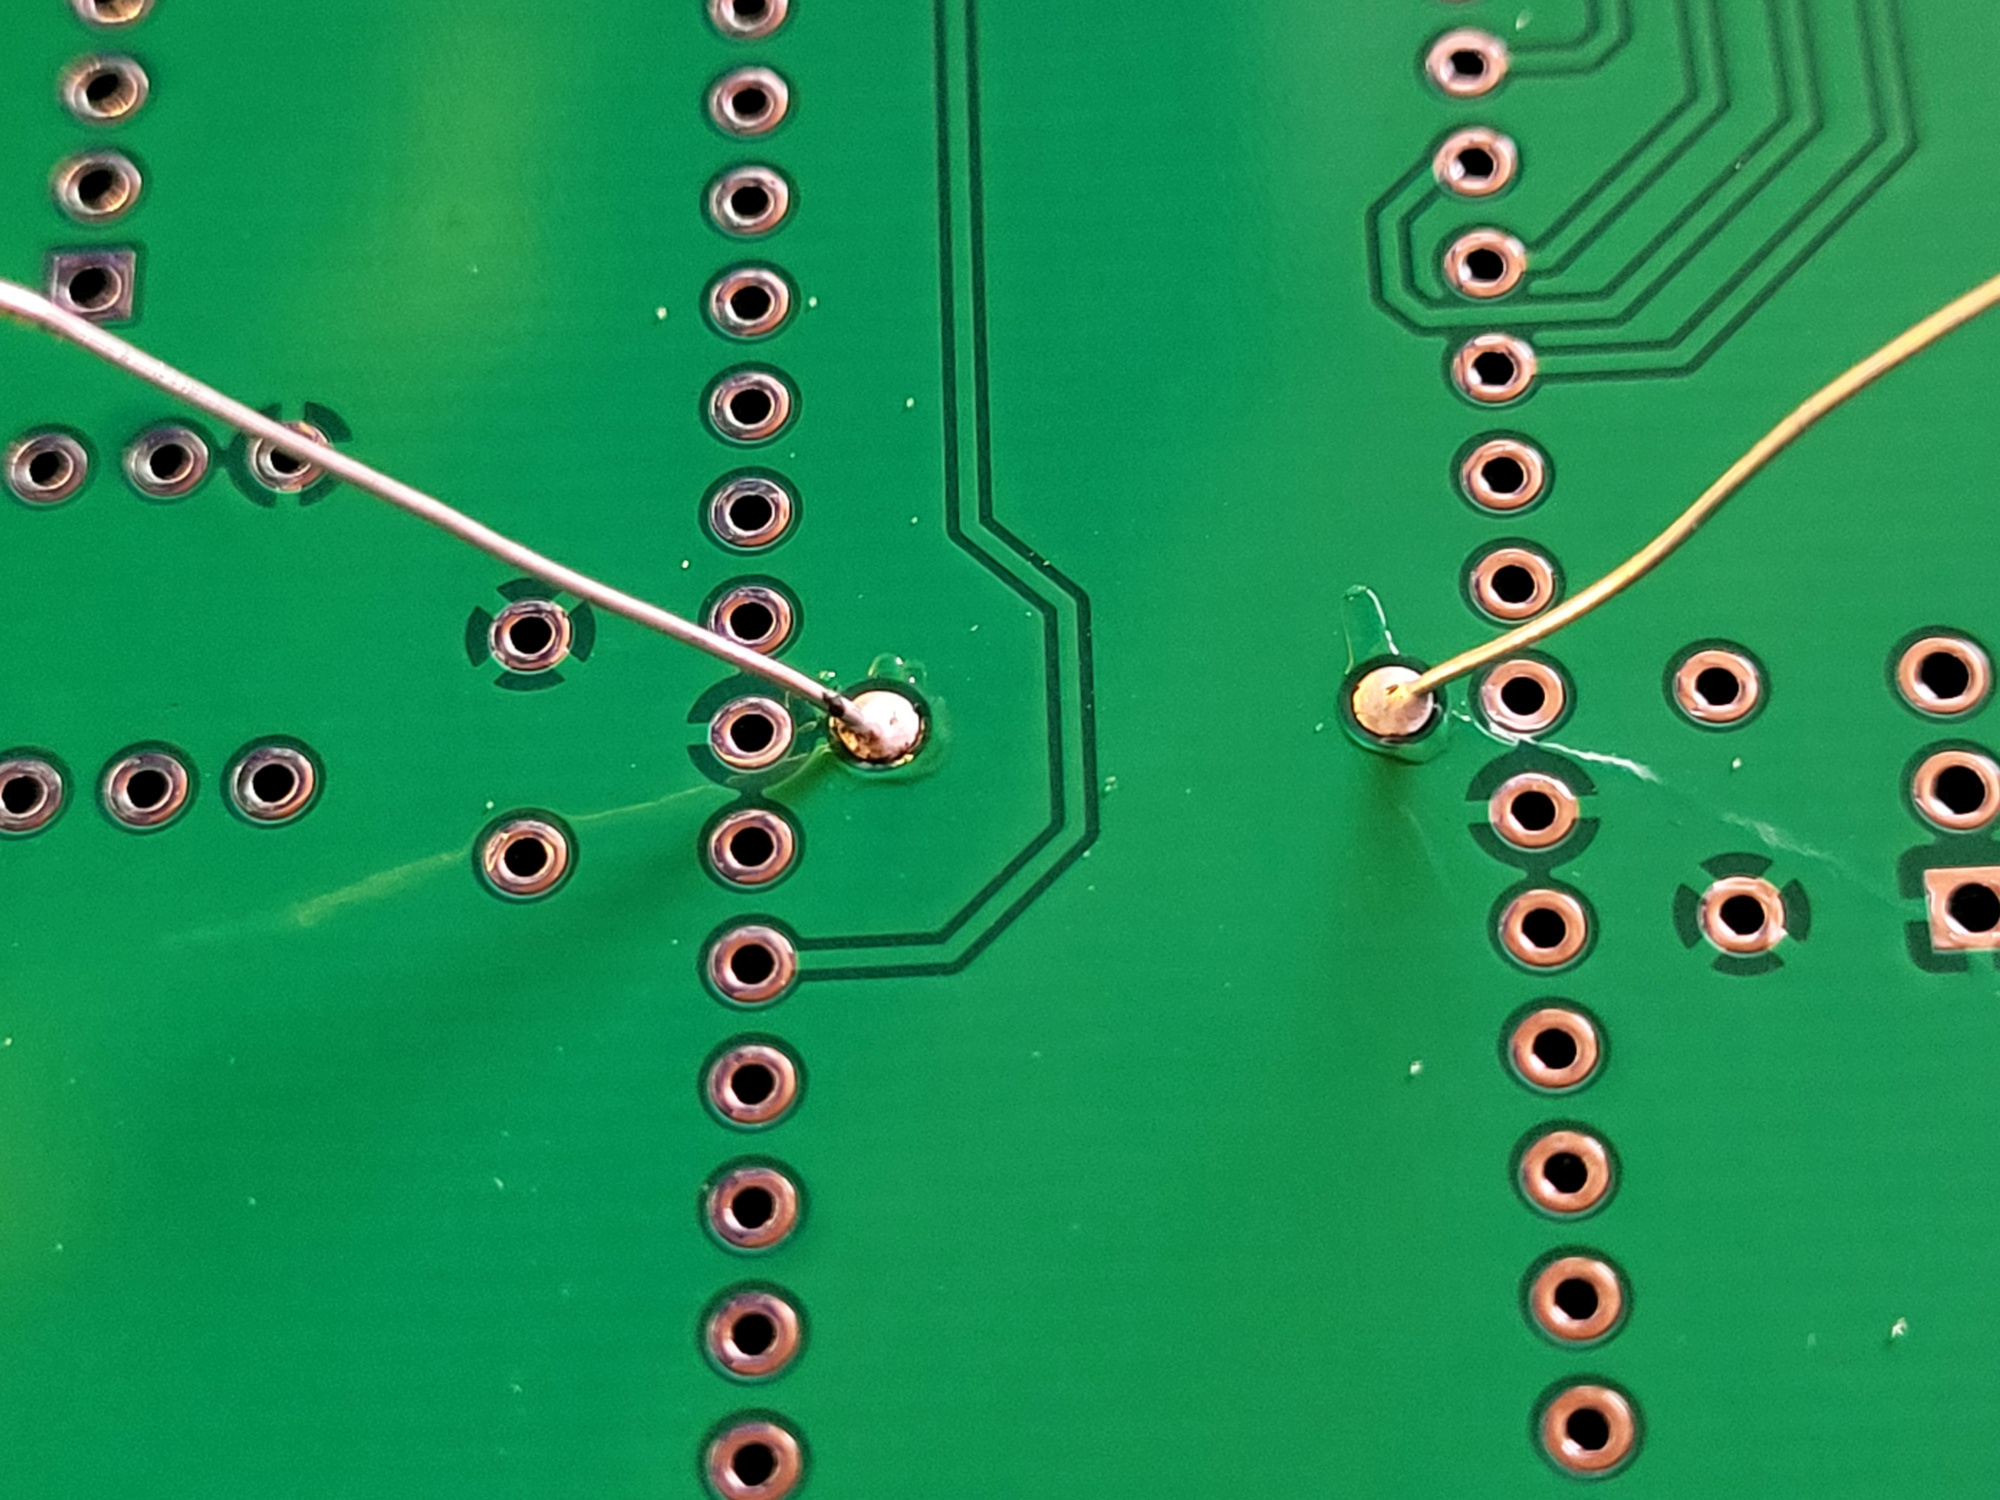
\includegraphics[width=0.85\textwidth]{Pictures/Solder3.jpg}
\caption{Step 3: Solder it in}
\label{fig:solder3}
\end{figure}
\begin{figure}[htb]
\centering
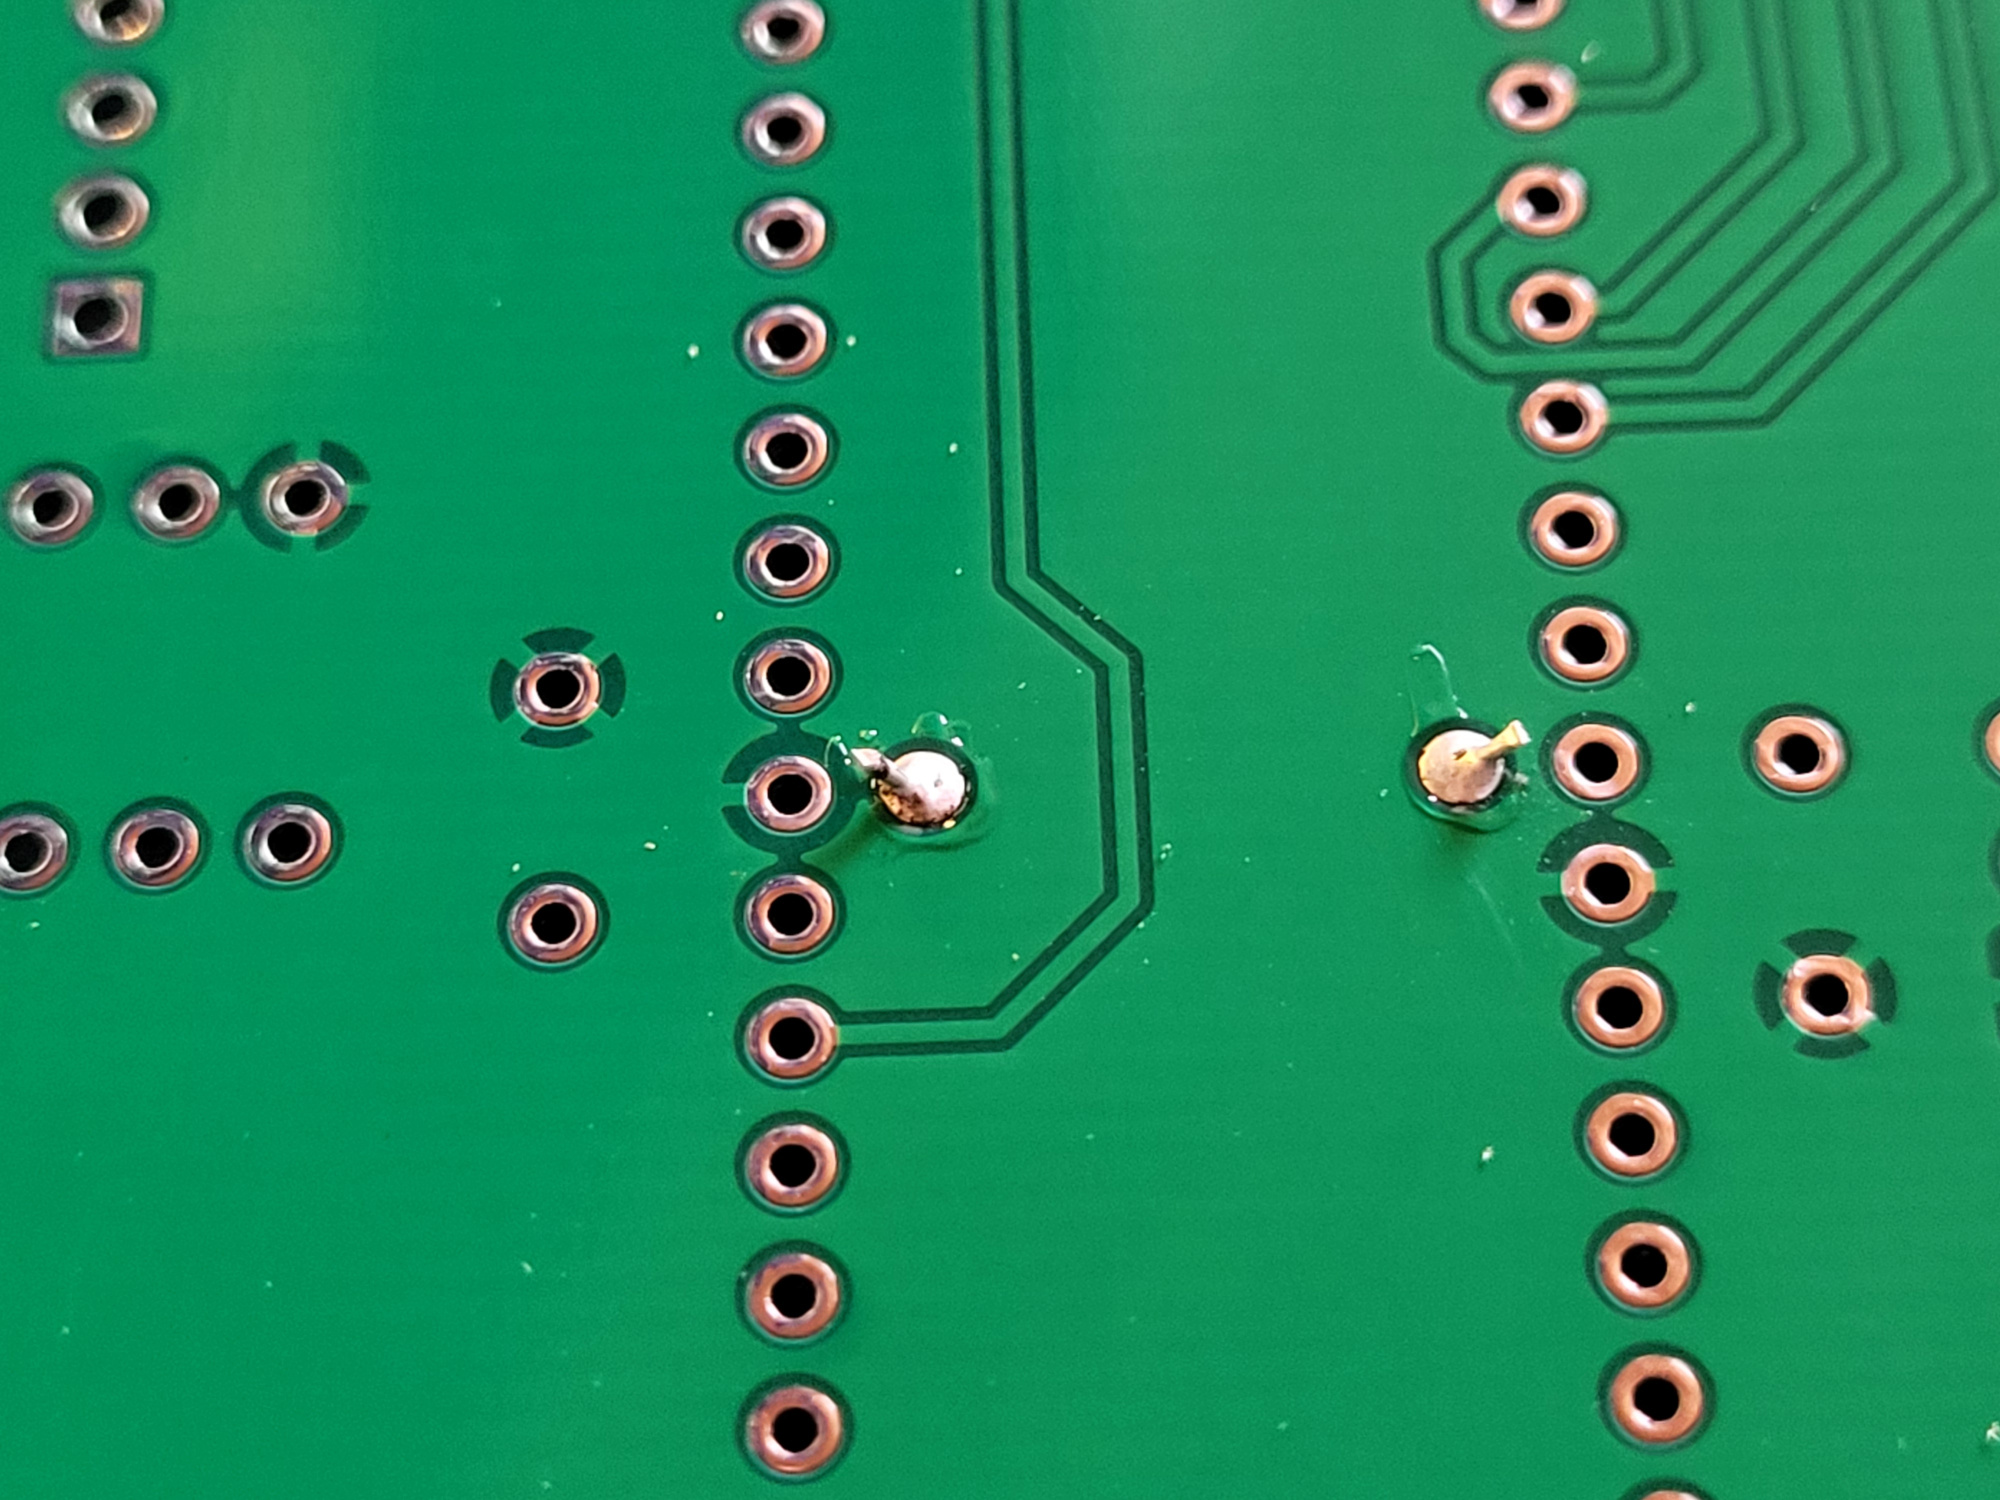
\includegraphics[width=0.85\textwidth]{Pictures/Solder4.jpg}
\caption{Cut off excess wire}
\label{fig:solder4}
\end{figure}

While the order in which you solder the components doesn't matter, it's probably a good idea to solder smaller components before taller, adjacent ones. 

\begin{caution}
The single exception is R1 which is placed underneath the IC socket for U1. Before soldering, make sure they fit on top of each other. If not, you can place R1 on the back of the board instead. 
\end{caution}

\subsubsection{Orientation of Components}
For most components, the orientation is crucial. Only for resistors (but not resistor networks), ceramic capacitors (but not electrolytic ones), crystrals (but not crystal oscillators), and pin headers/sockets it doesn't matter. Components mounted in the wrong orientation can get damaged and/or damage others. They might also emit smoke and catch fire. Here are some clues for how to properly orient components:

\begin{itemize}
\item Diodes: The anode is marked by a ring and so is the icon on the board
\item LEDs: The anode is on the round side of the casing and has the longer leg. It goes into the round pad of the PCB. The cathode is on the flat side of the casing and goes into the square pad of the PCB. 
\item Electrolytic capacitors: The plus side (longer leg) goes into the square pad marked ``+'' of the PCB. The minus side (shorter leg) goes into the round pad of the PCB. The minus side usually has a white marking, as does the PCB. \\
C7 is special, since it is axial (``lying down''). The correct orientation is determined by the groove. 
\item The resistor networks (RN1, RN2) consist internally of eight resistors with one end of each tied together (hence nine pins). The common pin (1) is usually marked with a small dot. If you're unsure, you can use a multimeter in resistance mode to verify which pin has 1.5kΩ to the eight other ones. 
\item ICs and IC sockets (U1, U2) have a half-circle marking on one side, as does the PCB. While the orientation of the socket technically doesn't matter, it is a good idea to solder it in this orientation to avoid later confusion. 
\item As sockets for crystal oscillators (Y1) are hard to come by, we use a standard 14-pin IC socket instead. In this case, the marking has no meaning, but be sure to plug the oscillator in the right way later (sharp corner at Pin 1). \\
Shorten the legs if it stands out too much. When using add-on boards, make sure their underside contacts don't touch the case of Y1 (or any other conductive part for that matter). 
\item Bridge rectifier (B1): One of the four legs is longer and marked with a ``+''. This leg goes into the square pad on the PCB, also marked ``+''. 
\item The voltage regulator (U3) needs to have its legs bent 90°. Use small pliers and make sure not to put physical stress onto the internals. The metal tab must lie on the exposed pad of the PCB (it functions as a small heat sink). You can solder the metal tab onto the PCB but if you're having trouble doing that, just screw it on. Don't risk damaging the regulator by soldering for too long. 
\end{itemize}

After soldering, you can wipe away flux residue with some alcohol (isopropyl is best but ethanol works too). 

\subsubsection{Optional Components}\label{sec:compOptional}
The spare connector (``SPARE CONN'') can be used to make 3-way connections or just as a repository for jumpers. It's convenient but not necessary. If you want to use it, solder an 8-long 2-row header and an 8-long 1-row header (or three 1-row headers) next to each other. 

There are two kinds of LCD that fit onto the board, as indicated by "LCD OPTION A" and "LCD OPTION B". On one, the backlight power supply pins ``A'' and ``K'' are next to DB7, on others they are on the other side, next to VSS (see Figure \ref{fig:lcds} for some examples). Check which option fits your LCD and solder the 16-pin socket into the corresponding pads, leaving the remaining two pads free. Alternatively, you can use an 18-pin socket which allows you to switch between both types later. 

\begin{note}
The pins ``A'' and ``K'' are sometimes called ``L+'' and ``L-'' or ``LED+'' and ``LED-'' or ``BL+'' and ``BL-'' or simply ``15'' and ``16''. 
\end{note}

\begin{figure}[htb]
\centering
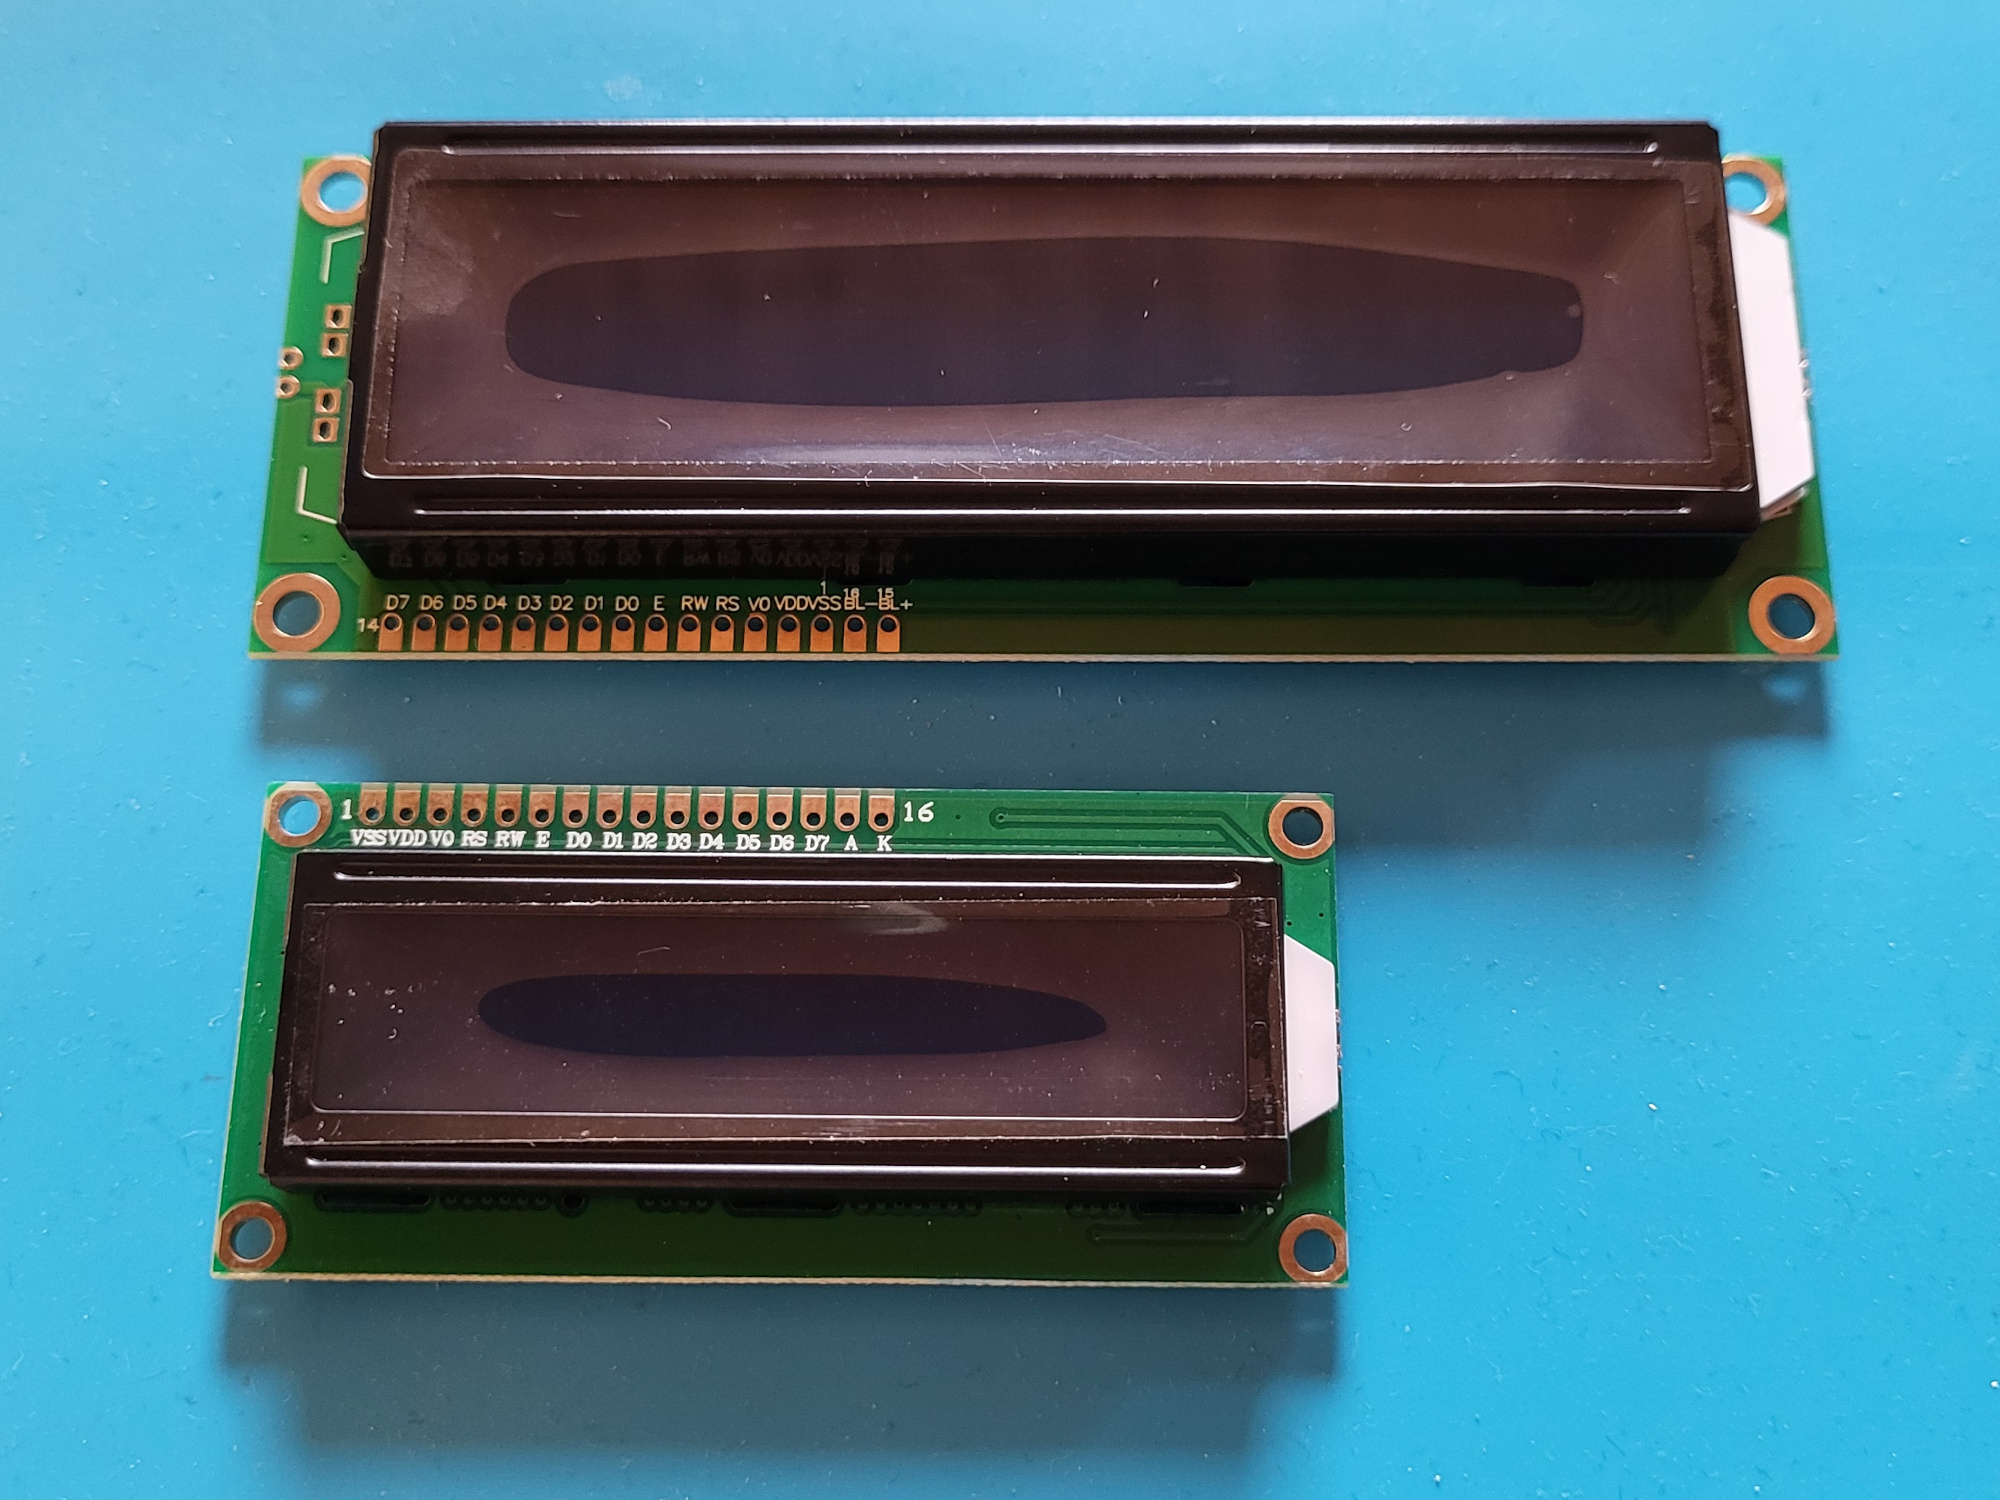
\includegraphics[width=0.85\textwidth]{Pictures/LCDs.jpg}
\caption{LCDs come in different sizes and with different pin layouts}
\label{fig:lcds}
\end{figure}

Resistors R30 and R31 are only necessary if your LCD crashes during programming, see Section \ref{sec:testLCD}. Unless and until that turns out to be a problem, you can leave them out. 
\FloatBarrier

\subsection{Testing (Part 1)}\label{sec:testingHardware}
If you have access to a multimeter, there are several things you can test before attaching the most vulnerable (and expensive) parts. Remove the ICs U1, U2, Y1 as well as the LCD from their sockets. Don't connect the power yet. 

First, use resistance or continuity mode to check the main nets. As an example, take the GND net: while holding one multimeter probe to one of the GND connectors (e.g.\ the top row pins of J3) place the other probe on all the other GND points: the VSS pin of J16, the GND pins of J8 and J9, pins 11 and 31 of U1, pin 15 of U2, pins 1 and 7 of Y1, and many more. Use KiCAD's PCB Editor to identify all the points. Do the same for the VCC net and -- if you want to be thorough -- for all other nets, especially the one involving the programming connectors (J8 and J9). 
\begin{figure}[htb]
\centering
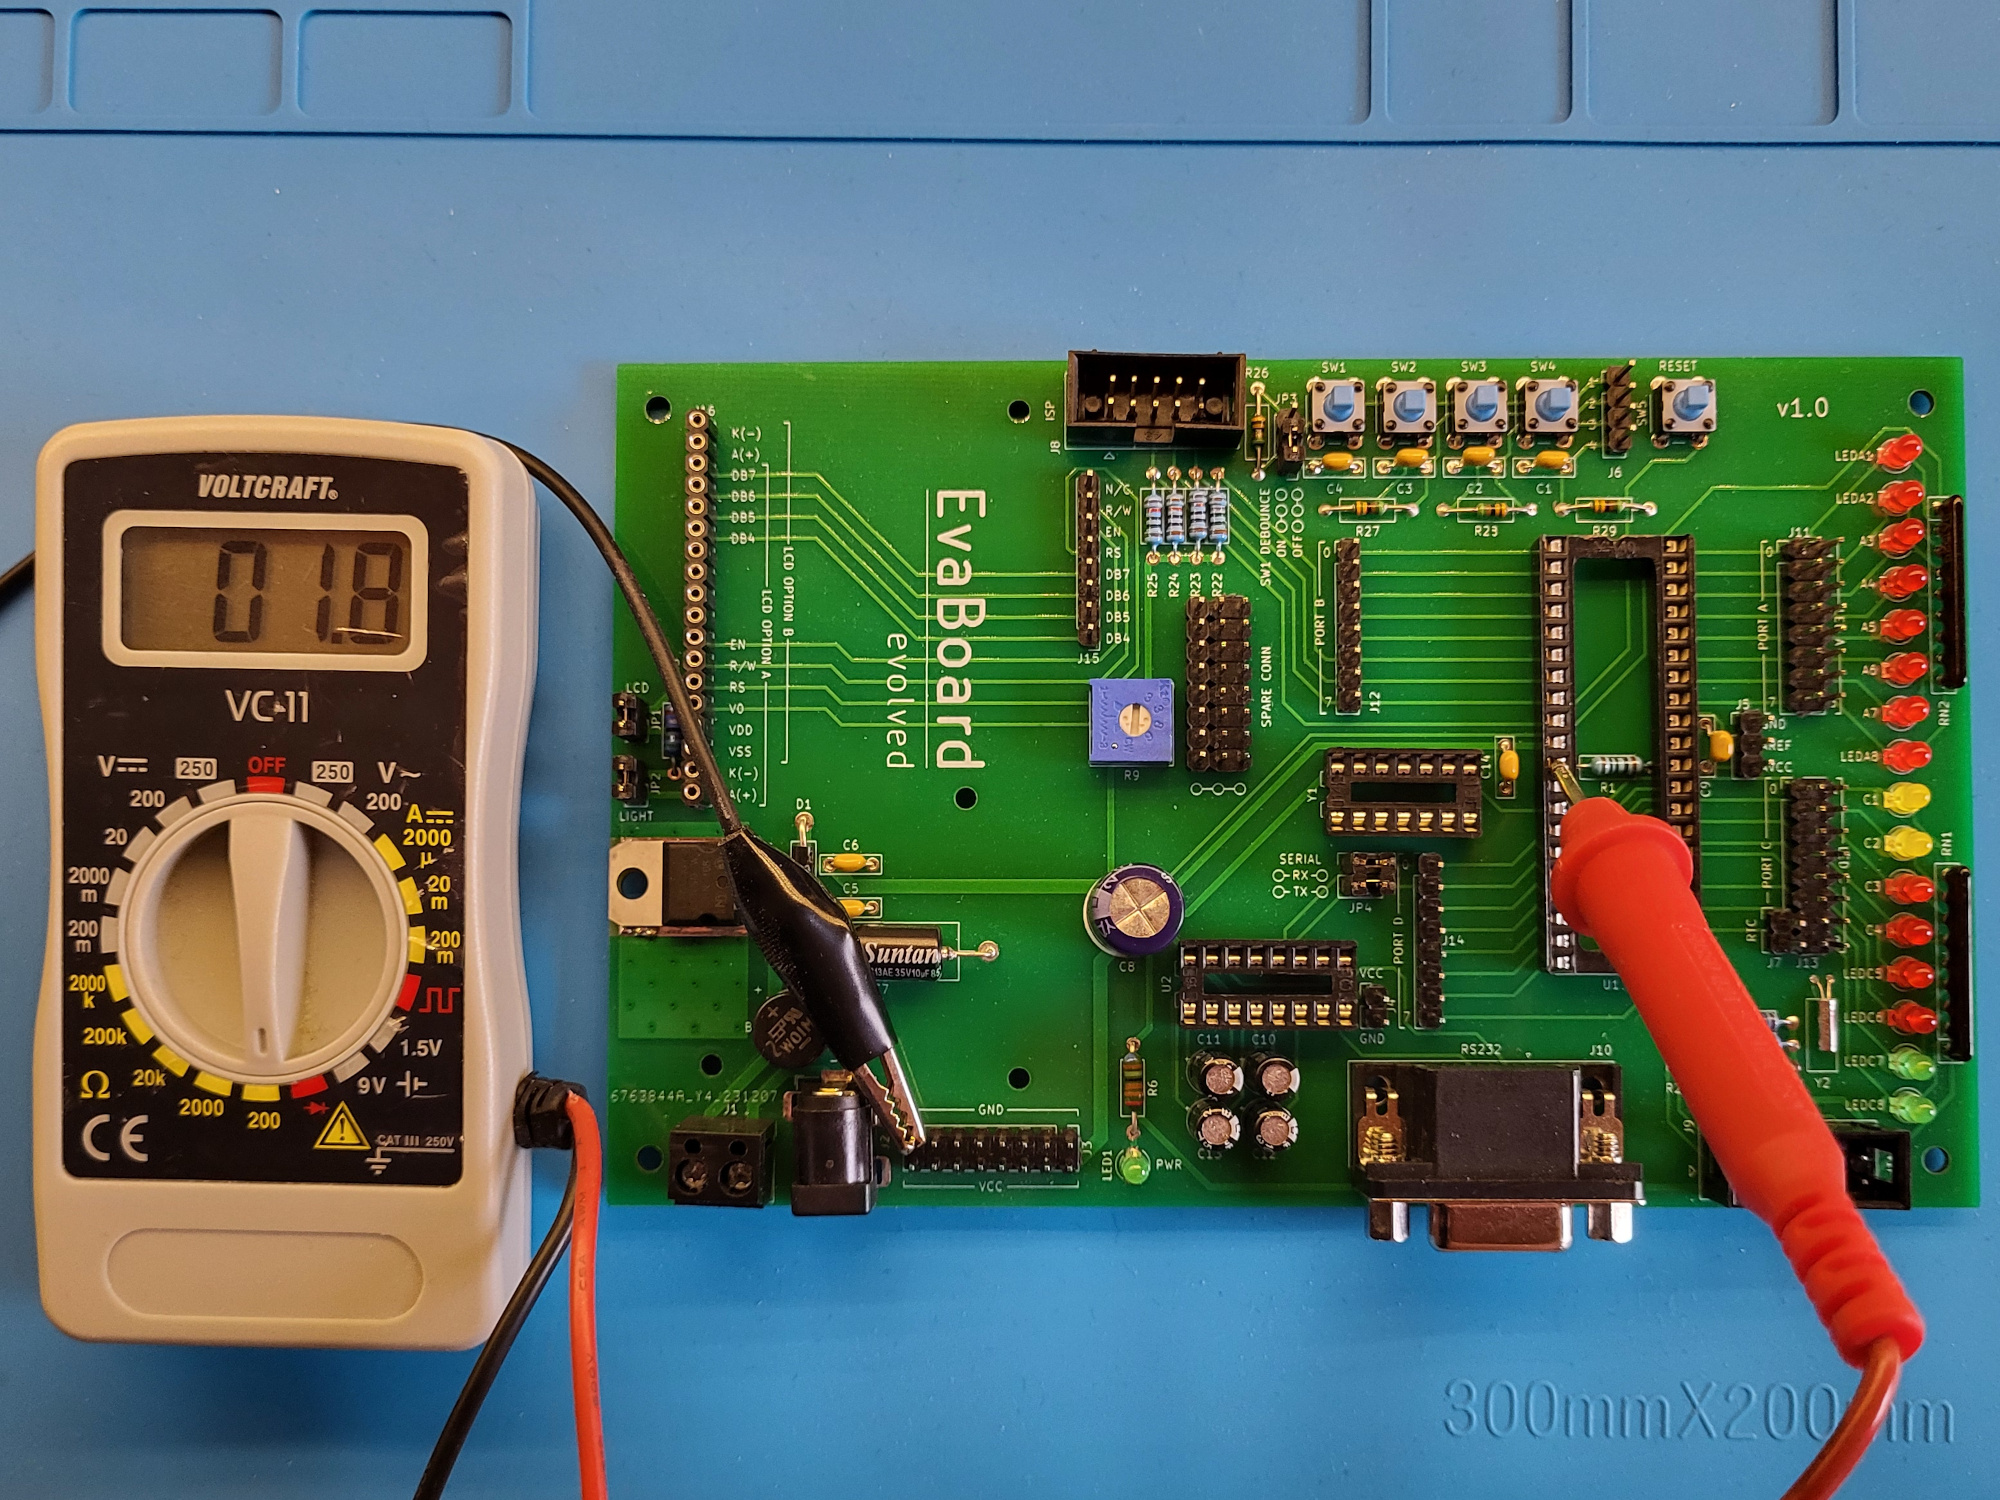
\includegraphics[width=0.85\textwidth]{Pictures/Testing1.jpg}
\caption{Continuity/Resistance Testing\\(The $1.8\Omega$ is due to bad multimeter calibration, in actuality it is almost $0\Omega$)}
\label{fig:testing1}
\end{figure}

Perhaps even more importantly, make sure that different nets like VCC and GND are NOT connected to each other. 

If a connection is missing, identify the faulty solder joint and redo it. 

Once you're satisfied, apply power to the board. LED1 (PWR) should light up. Check if anything gets hot. If so, unplug the power immediately and re-do the previous checks. 

Put the multimeter into voltage mode (if necessary, select a range above 5V) and measure the voltage between VCC and GND. It should be near 5V. If it is significantly lower, disconnect the power and look for a short. Be careful not to cause a short with the probes while measuring. 
\begin{figure}[htb]
\centering
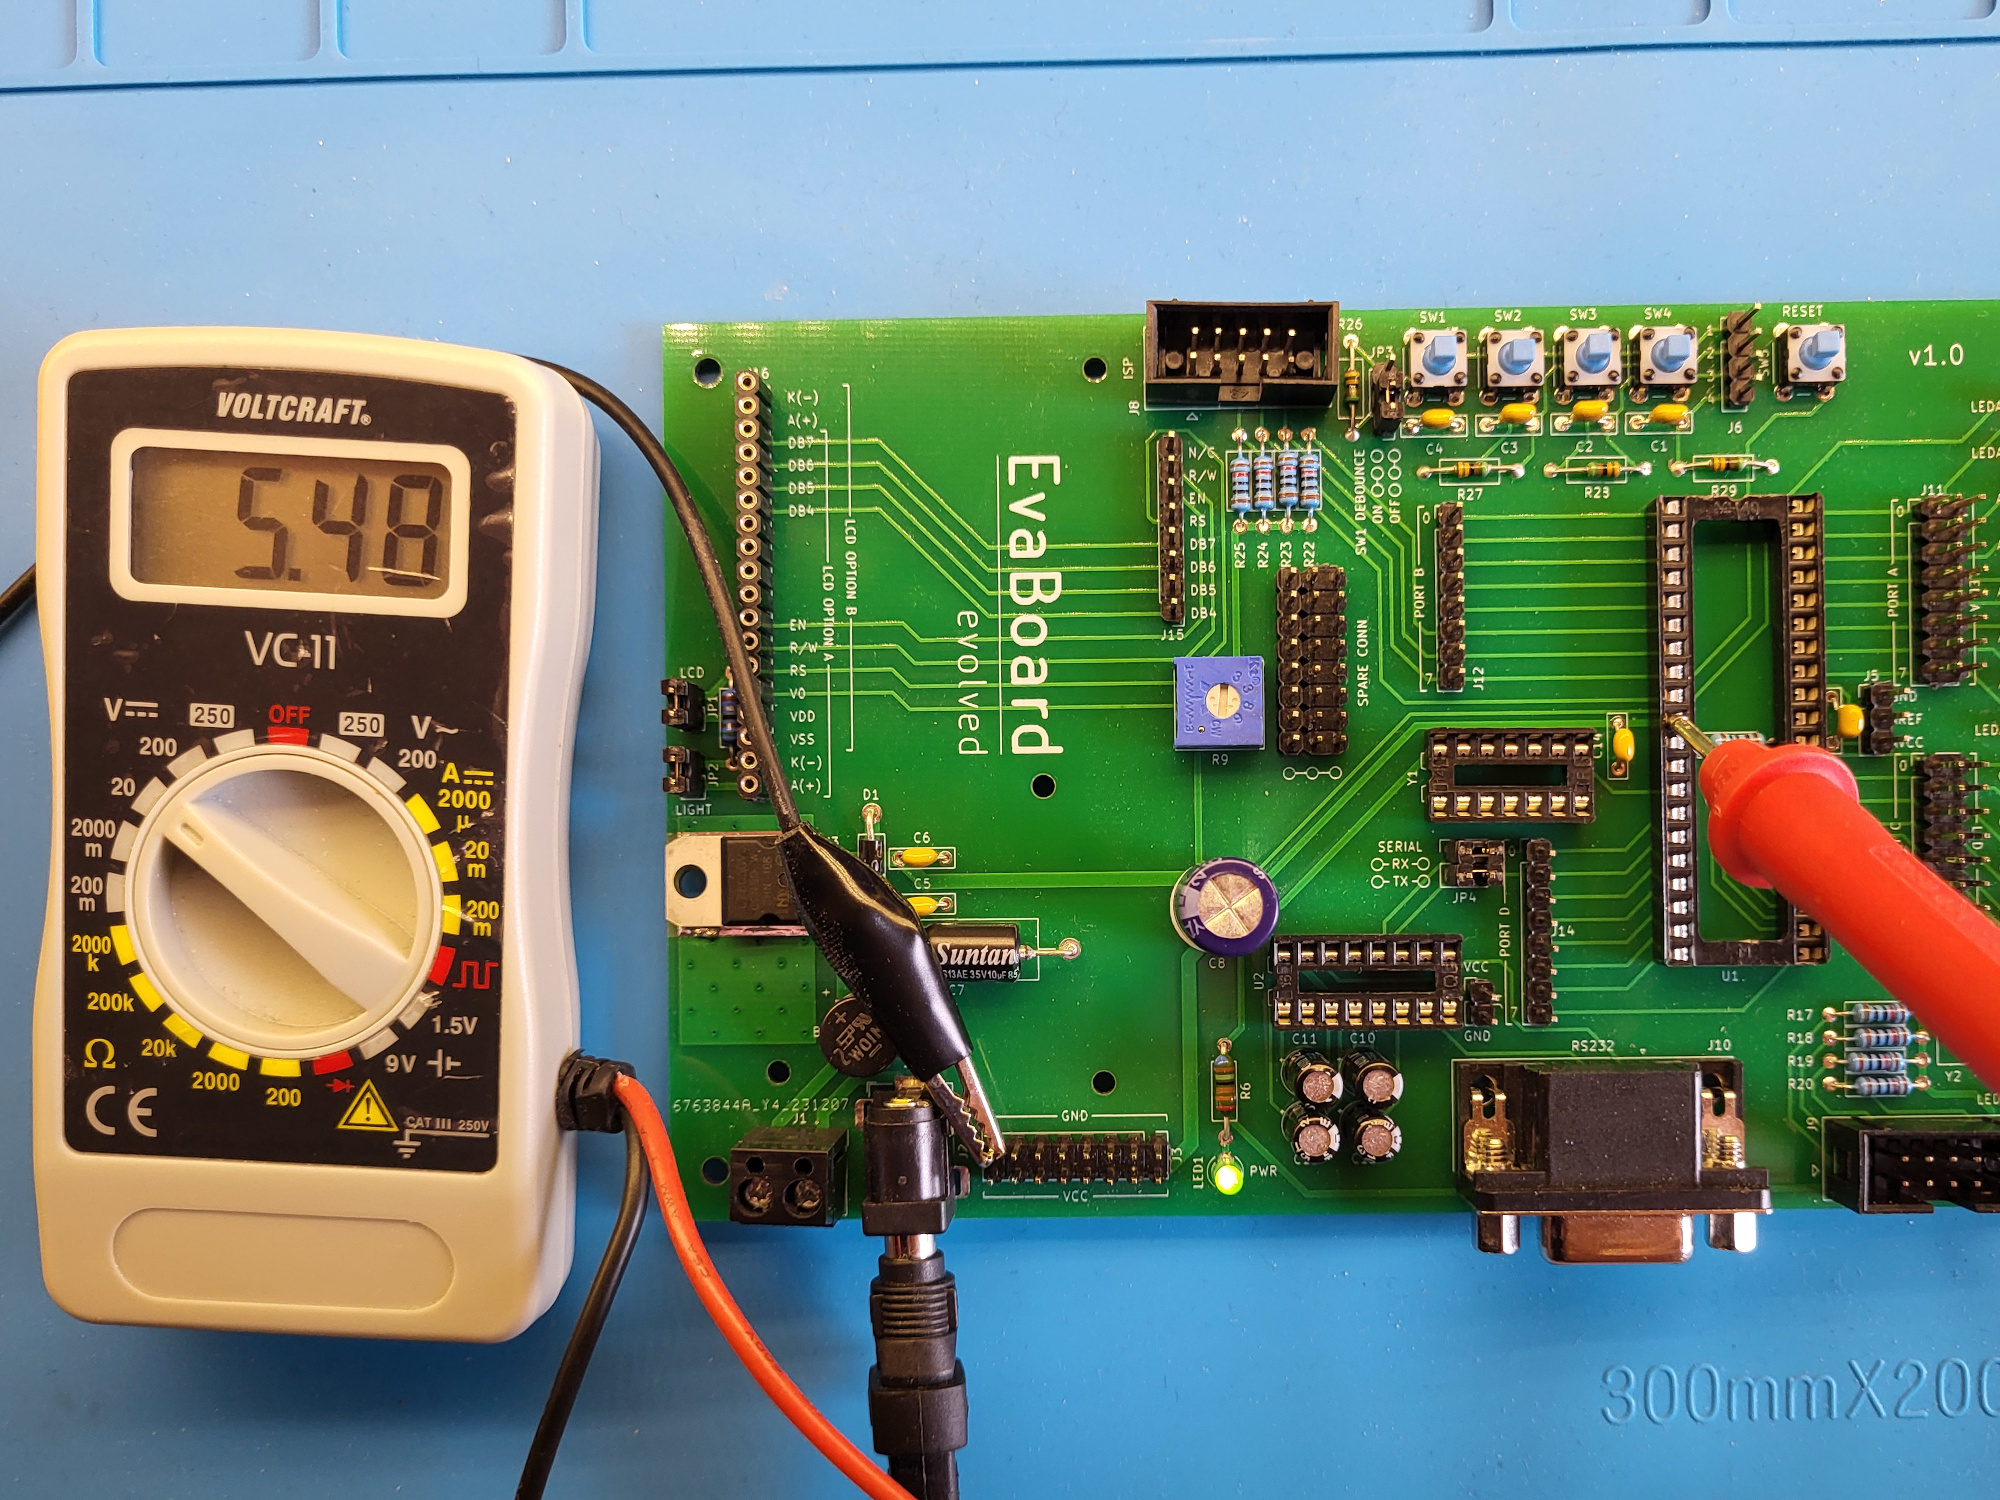
\includegraphics[width=0.85\textwidth]{Pictures/Testing2.jpg}
\caption{Voltage Testing (Again, the indicated $5.48V$ is in reality $5V$)}
\label{fig:testing2}
\end{figure}

You can manually test the LEDs using a jumper cable. Plug one end into one one of the LED pins (right column of J11 and J13) and connect the other end to GND (top row of J3). The LED should light up. 
\begin{figure}[htb]
\centering
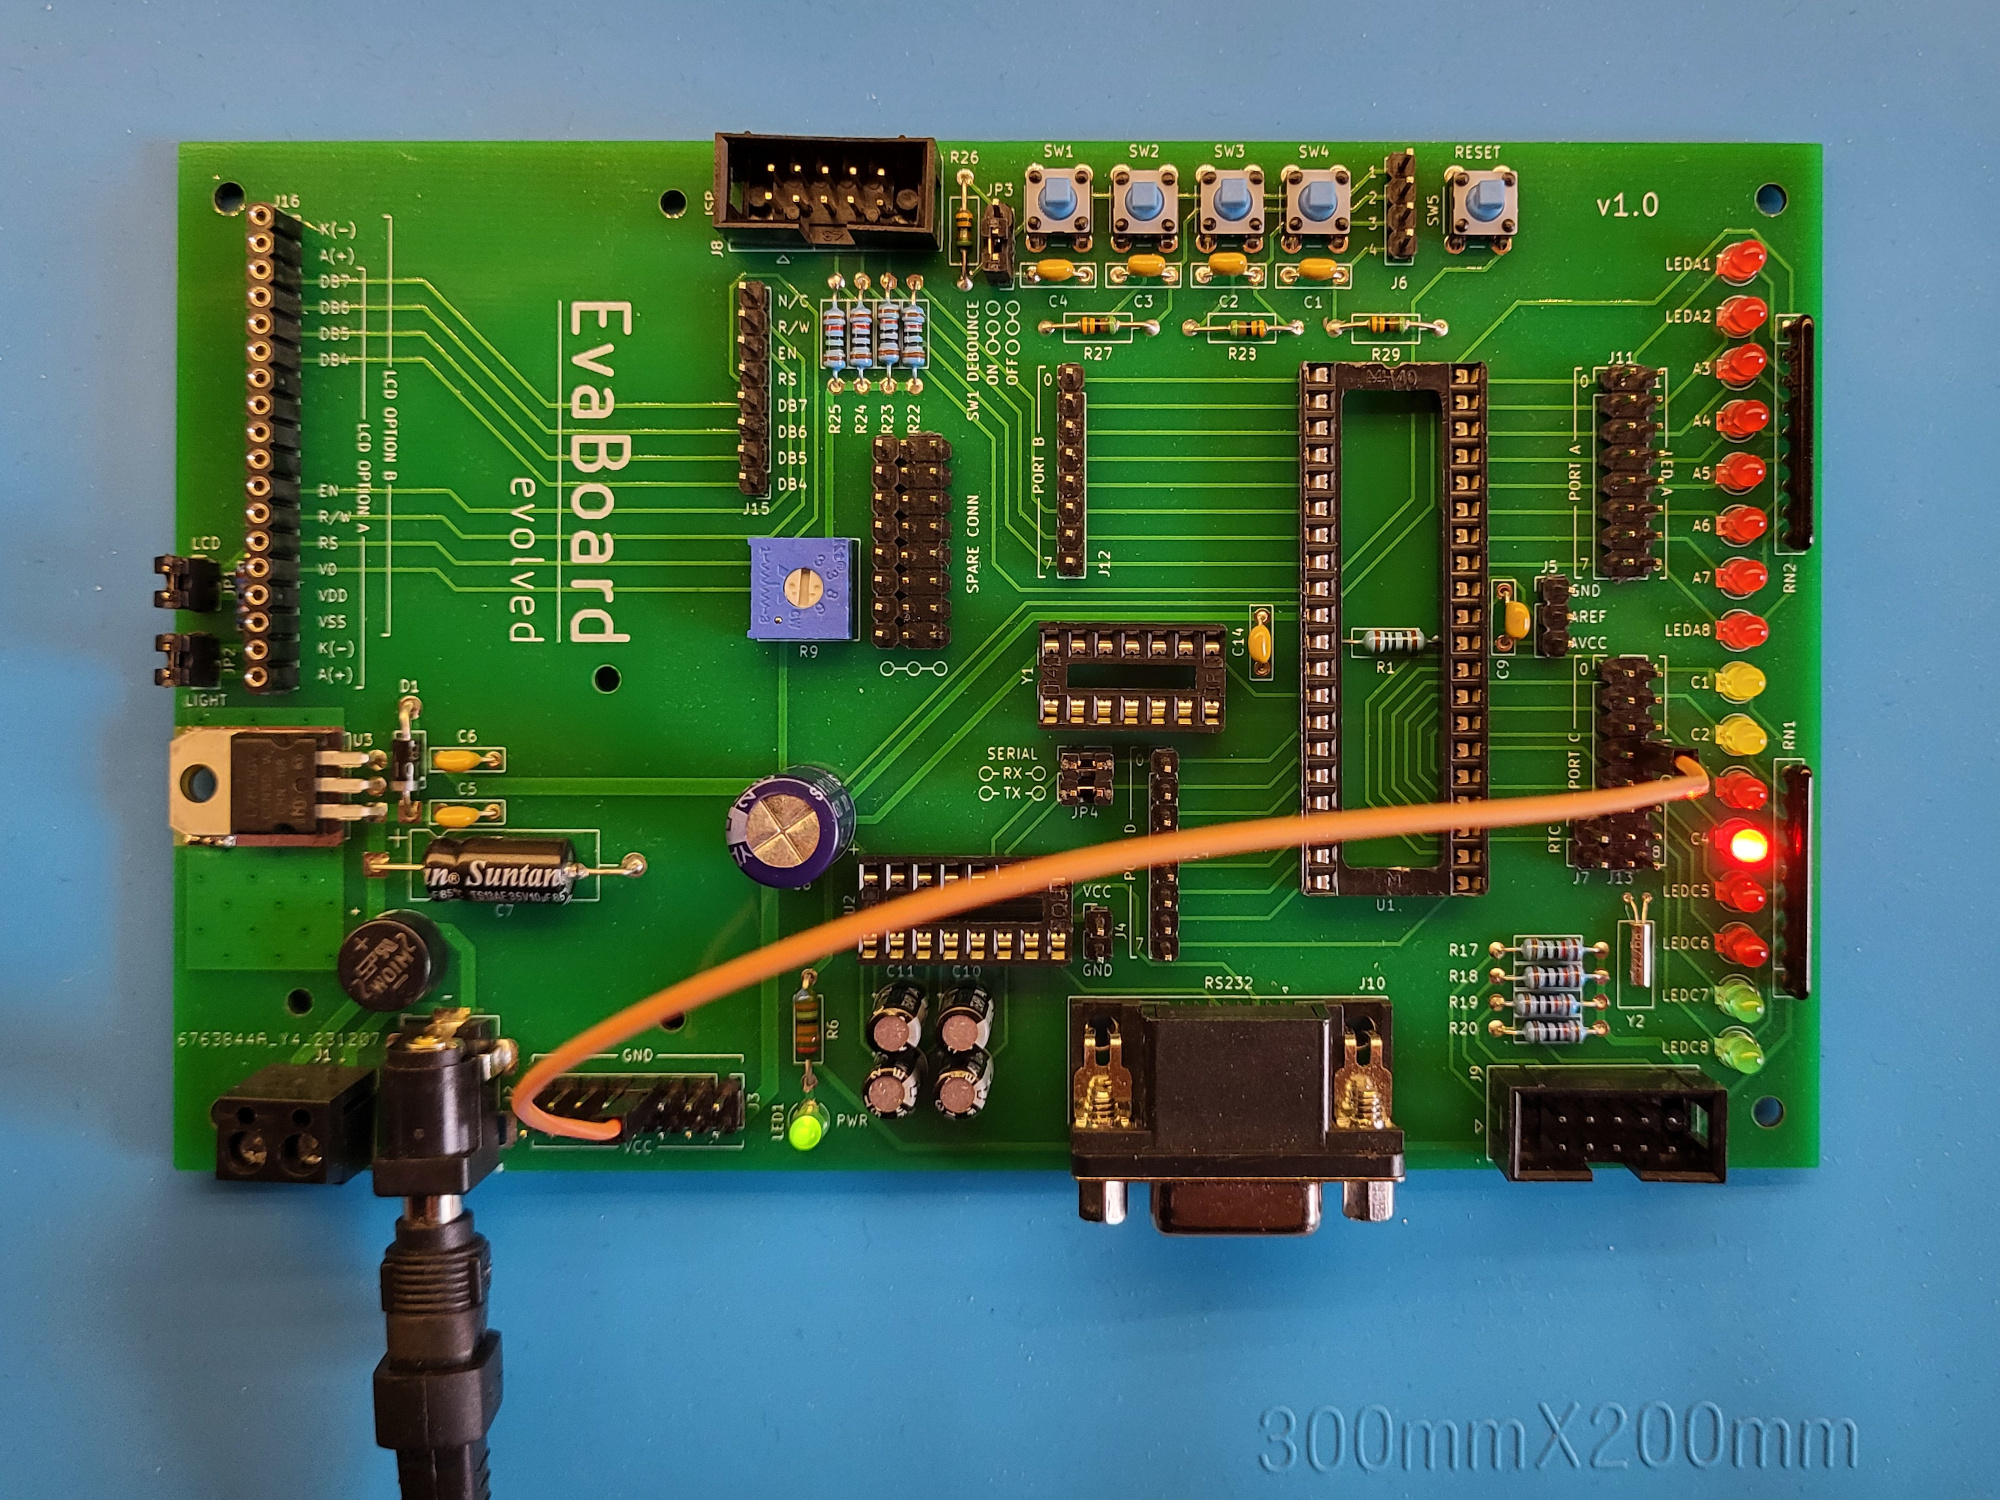
\includegraphics[width=0.85\textwidth]{Pictures/Testing3.jpg}
\caption{Testing the LEDs using a jumper cable}
\label{fig:testing3}
\end{figure}

The buttons can also be tested manually: Again using a jumper cable, connect one of the LED pins and one of the button pins (J6). The LED should light up while the button is pressed. 
\begin{figure}[htb]
\centering
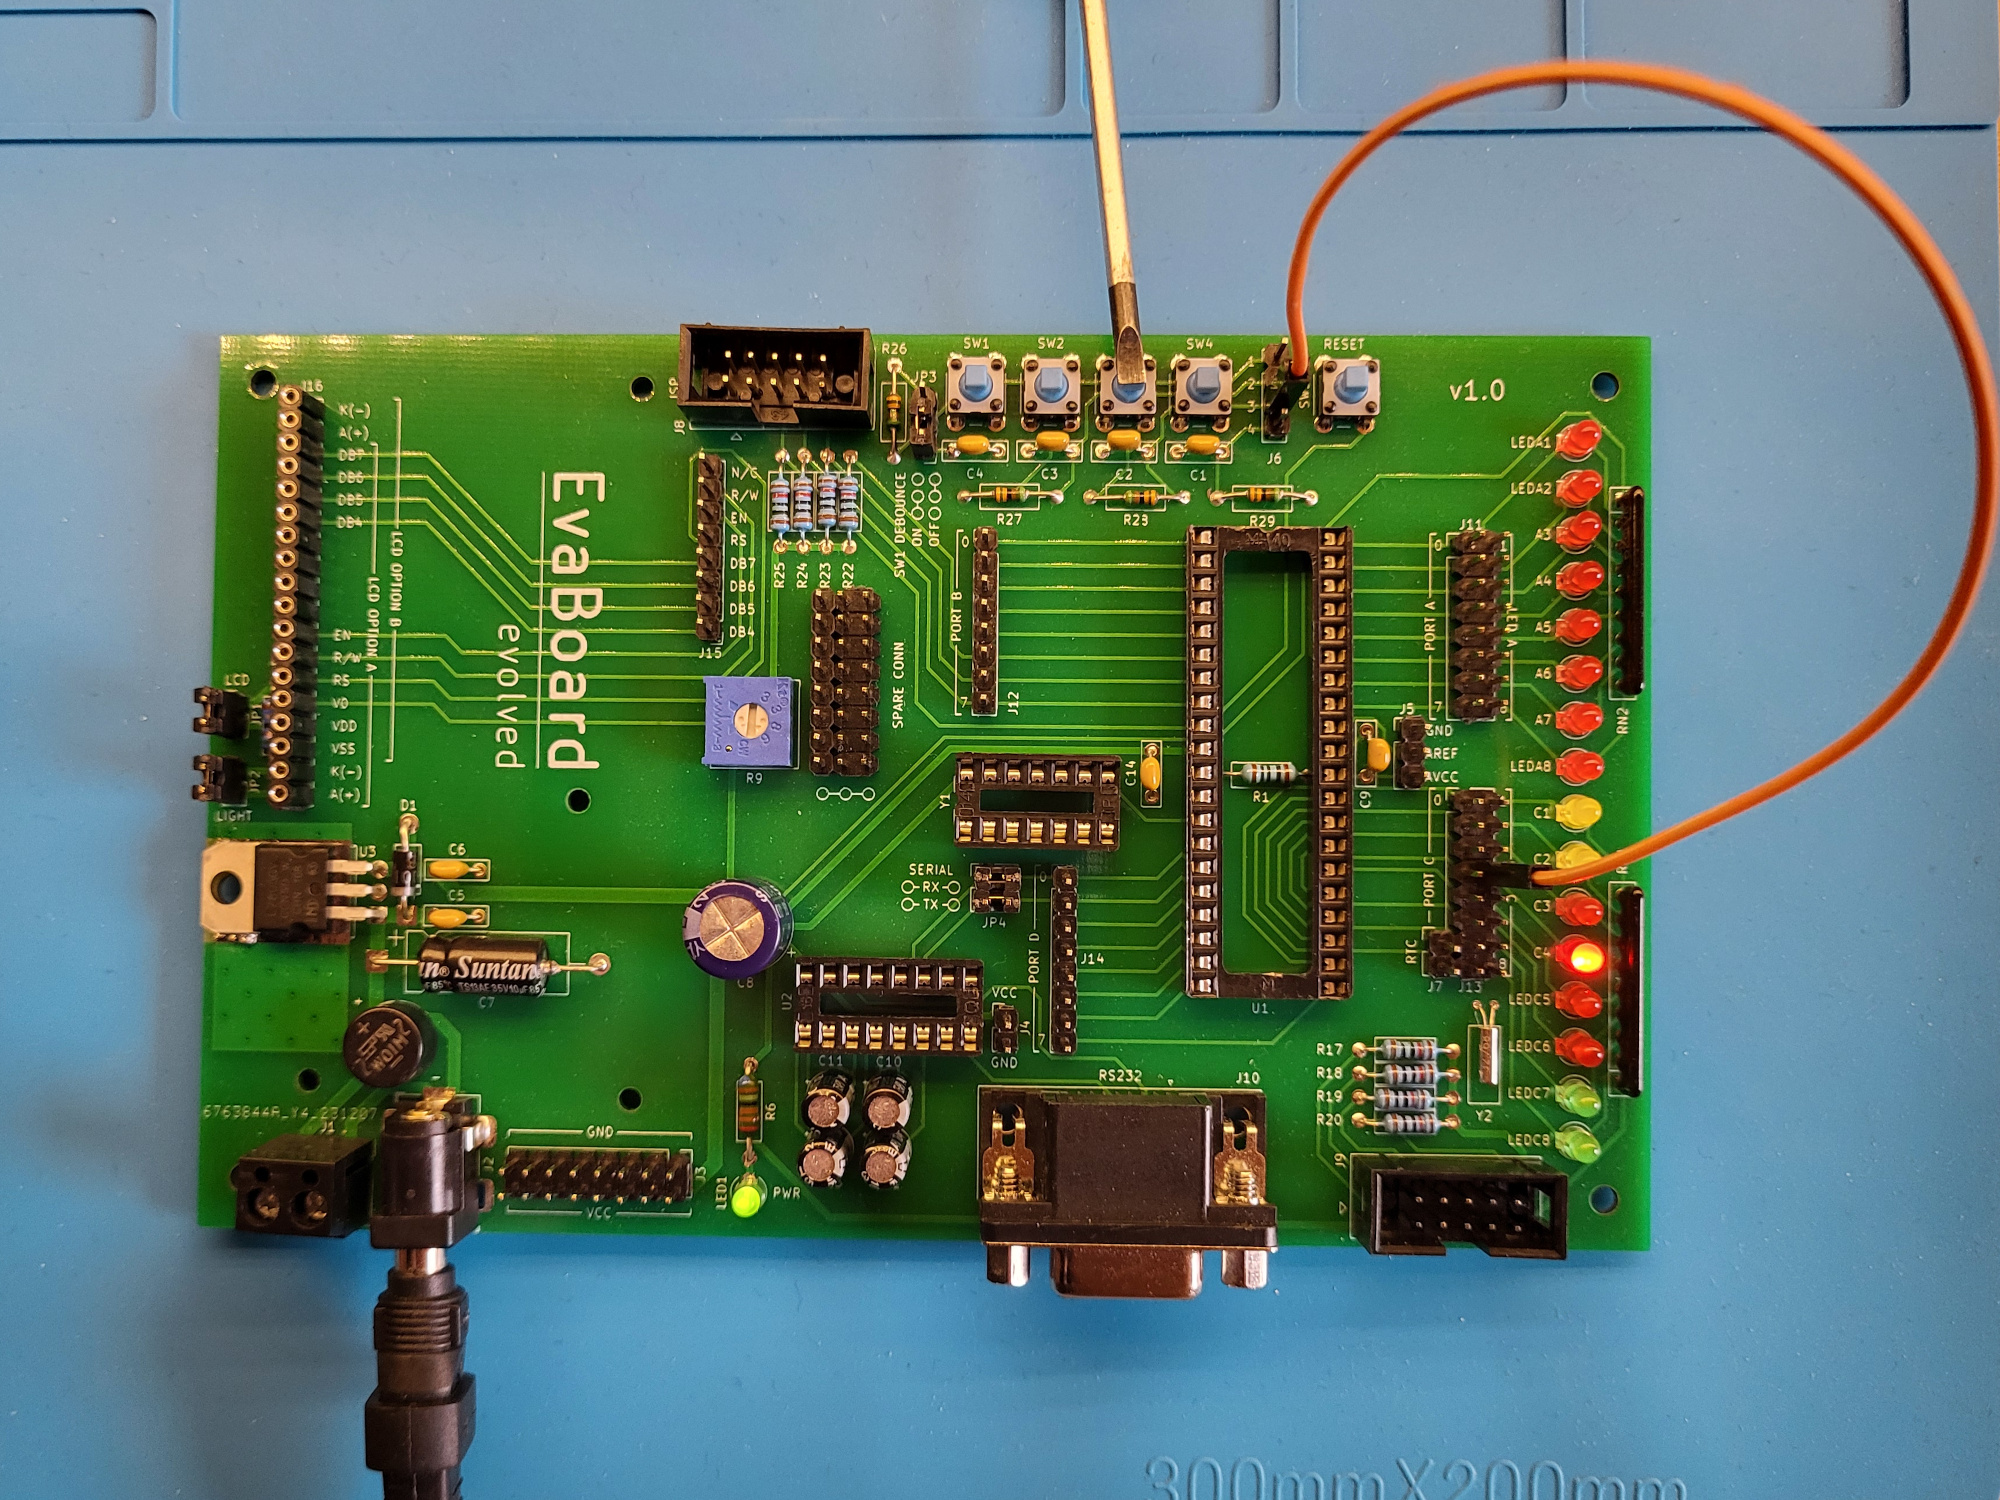
\includegraphics[width=0.85\textwidth]{Pictures/Testing4.jpg}
\caption{Testing the buttons using a jumper cable}
\label{fig:testing4}
\end{figure}

Insert the LCD and mount jumpers on LCD (JP1) and LIGHT (JP2). Since no one is sending commands to it, it should show the default pattern: all pixels in the first line on, all pixels in the second line off. You will probably need to adjust the contrast on R9 with a screwdriver before the pattern becomes visible. 
\begin{figure}[htb]
\centering
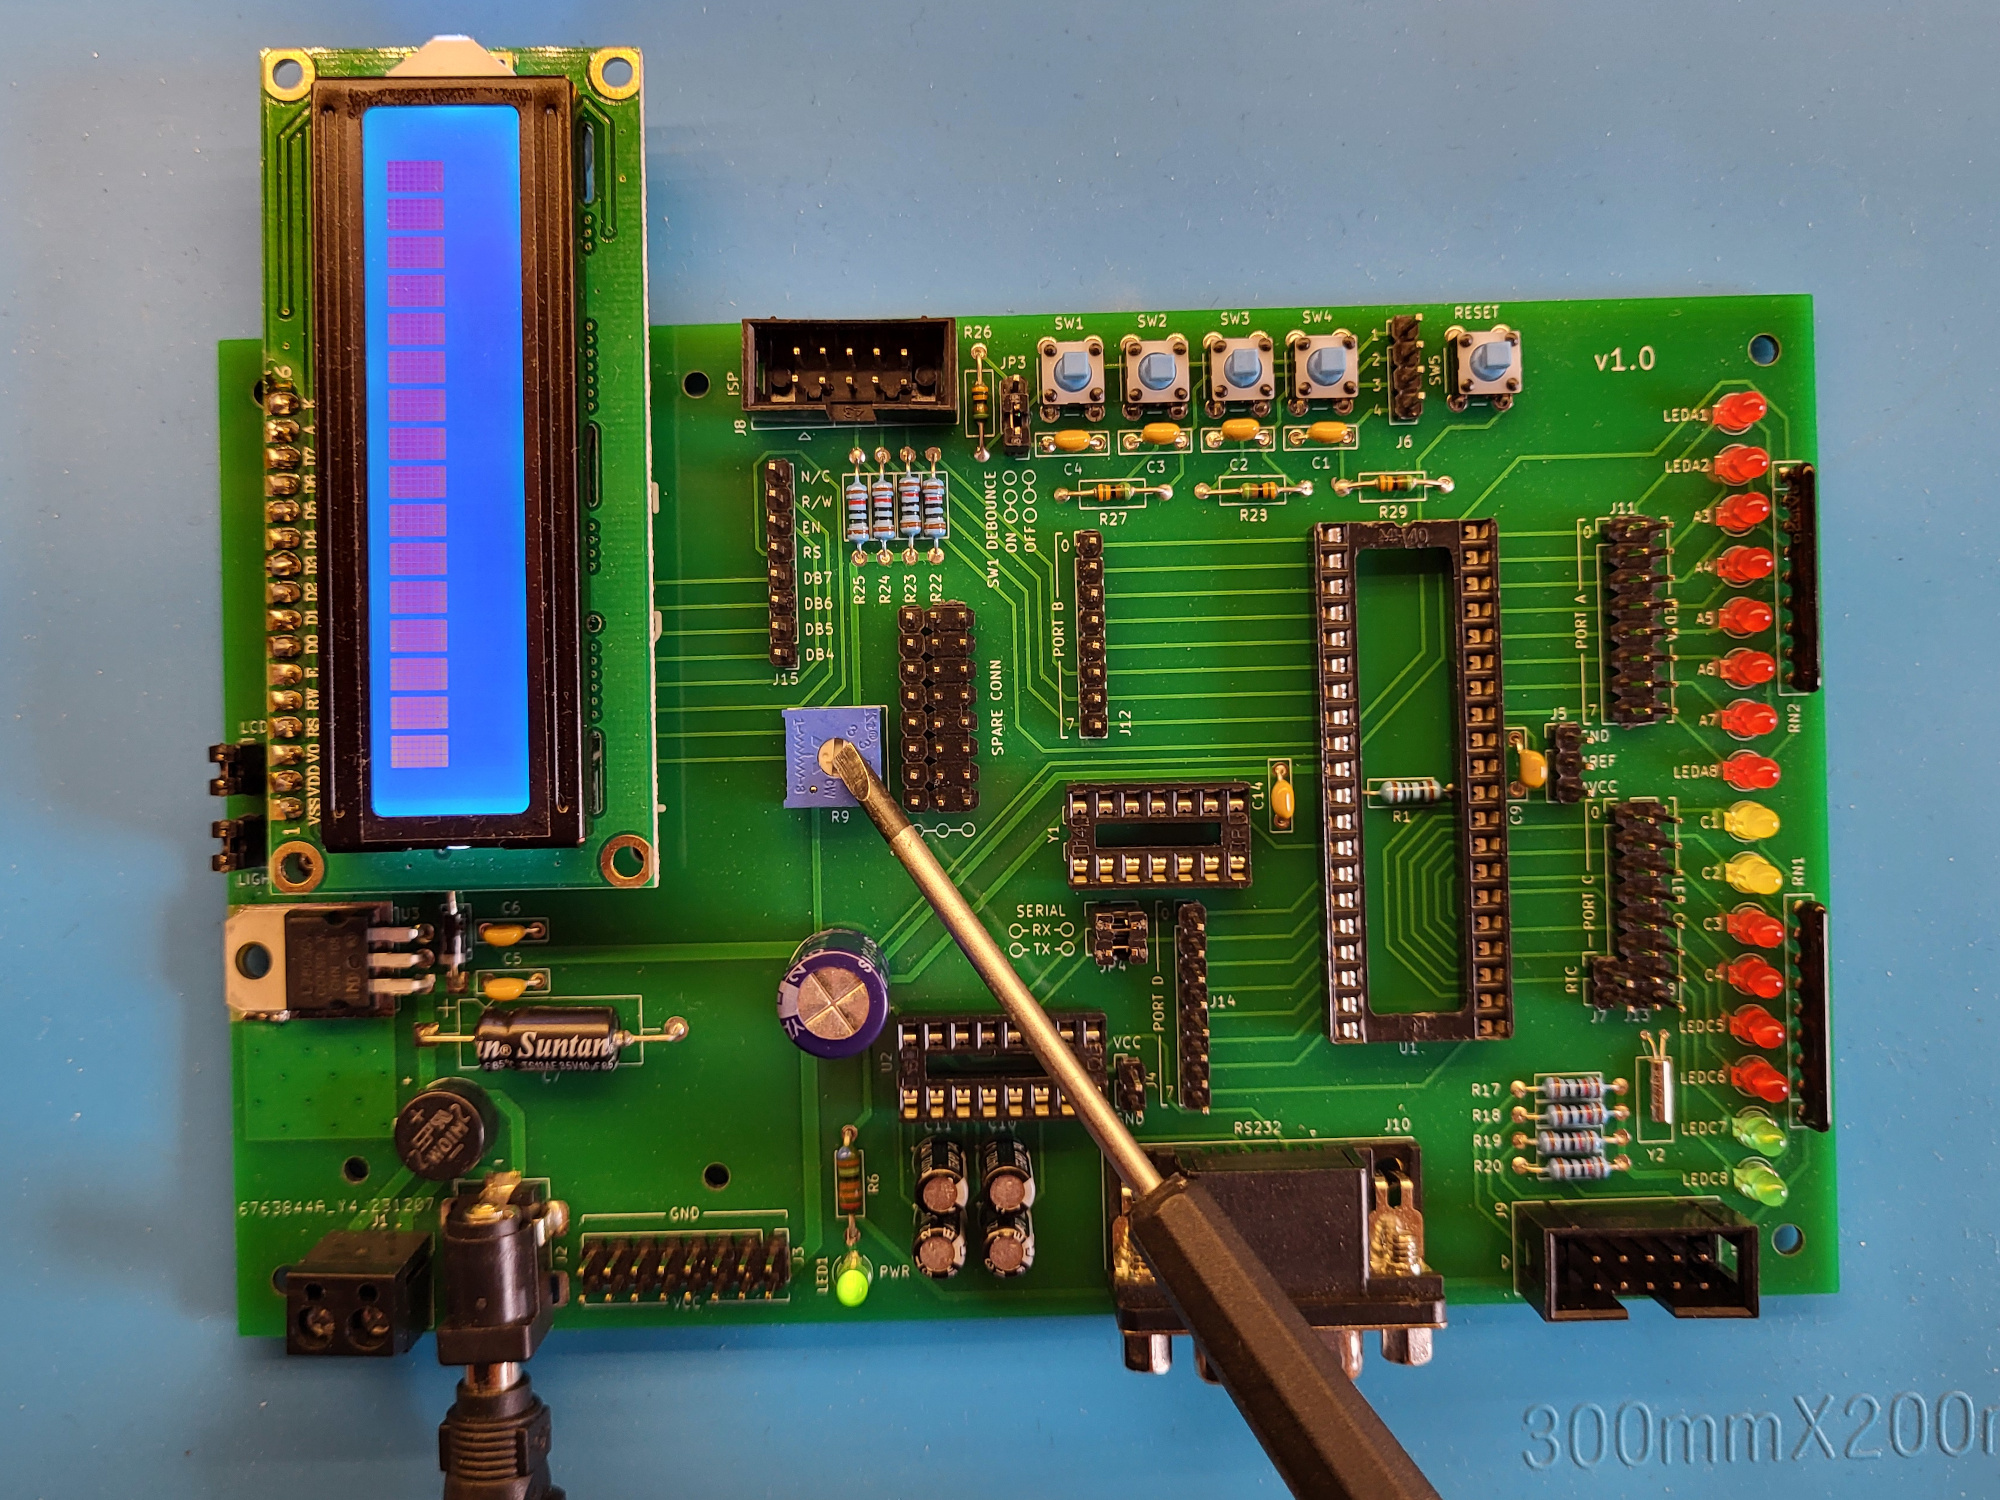
\includegraphics[width=0.85\textwidth]{Pictures/Testing5.jpg}
\caption{Setting the contrast voltage for the LCD}
\label{fig:testing5}
\end{figure}

If everything looks good, unplug the power and finish the board by inserting the missing ICs. Mount a jumper on SW1 DEBOUNCE ON (left position of JP3). 
\begin{figure}[htb]
\centering
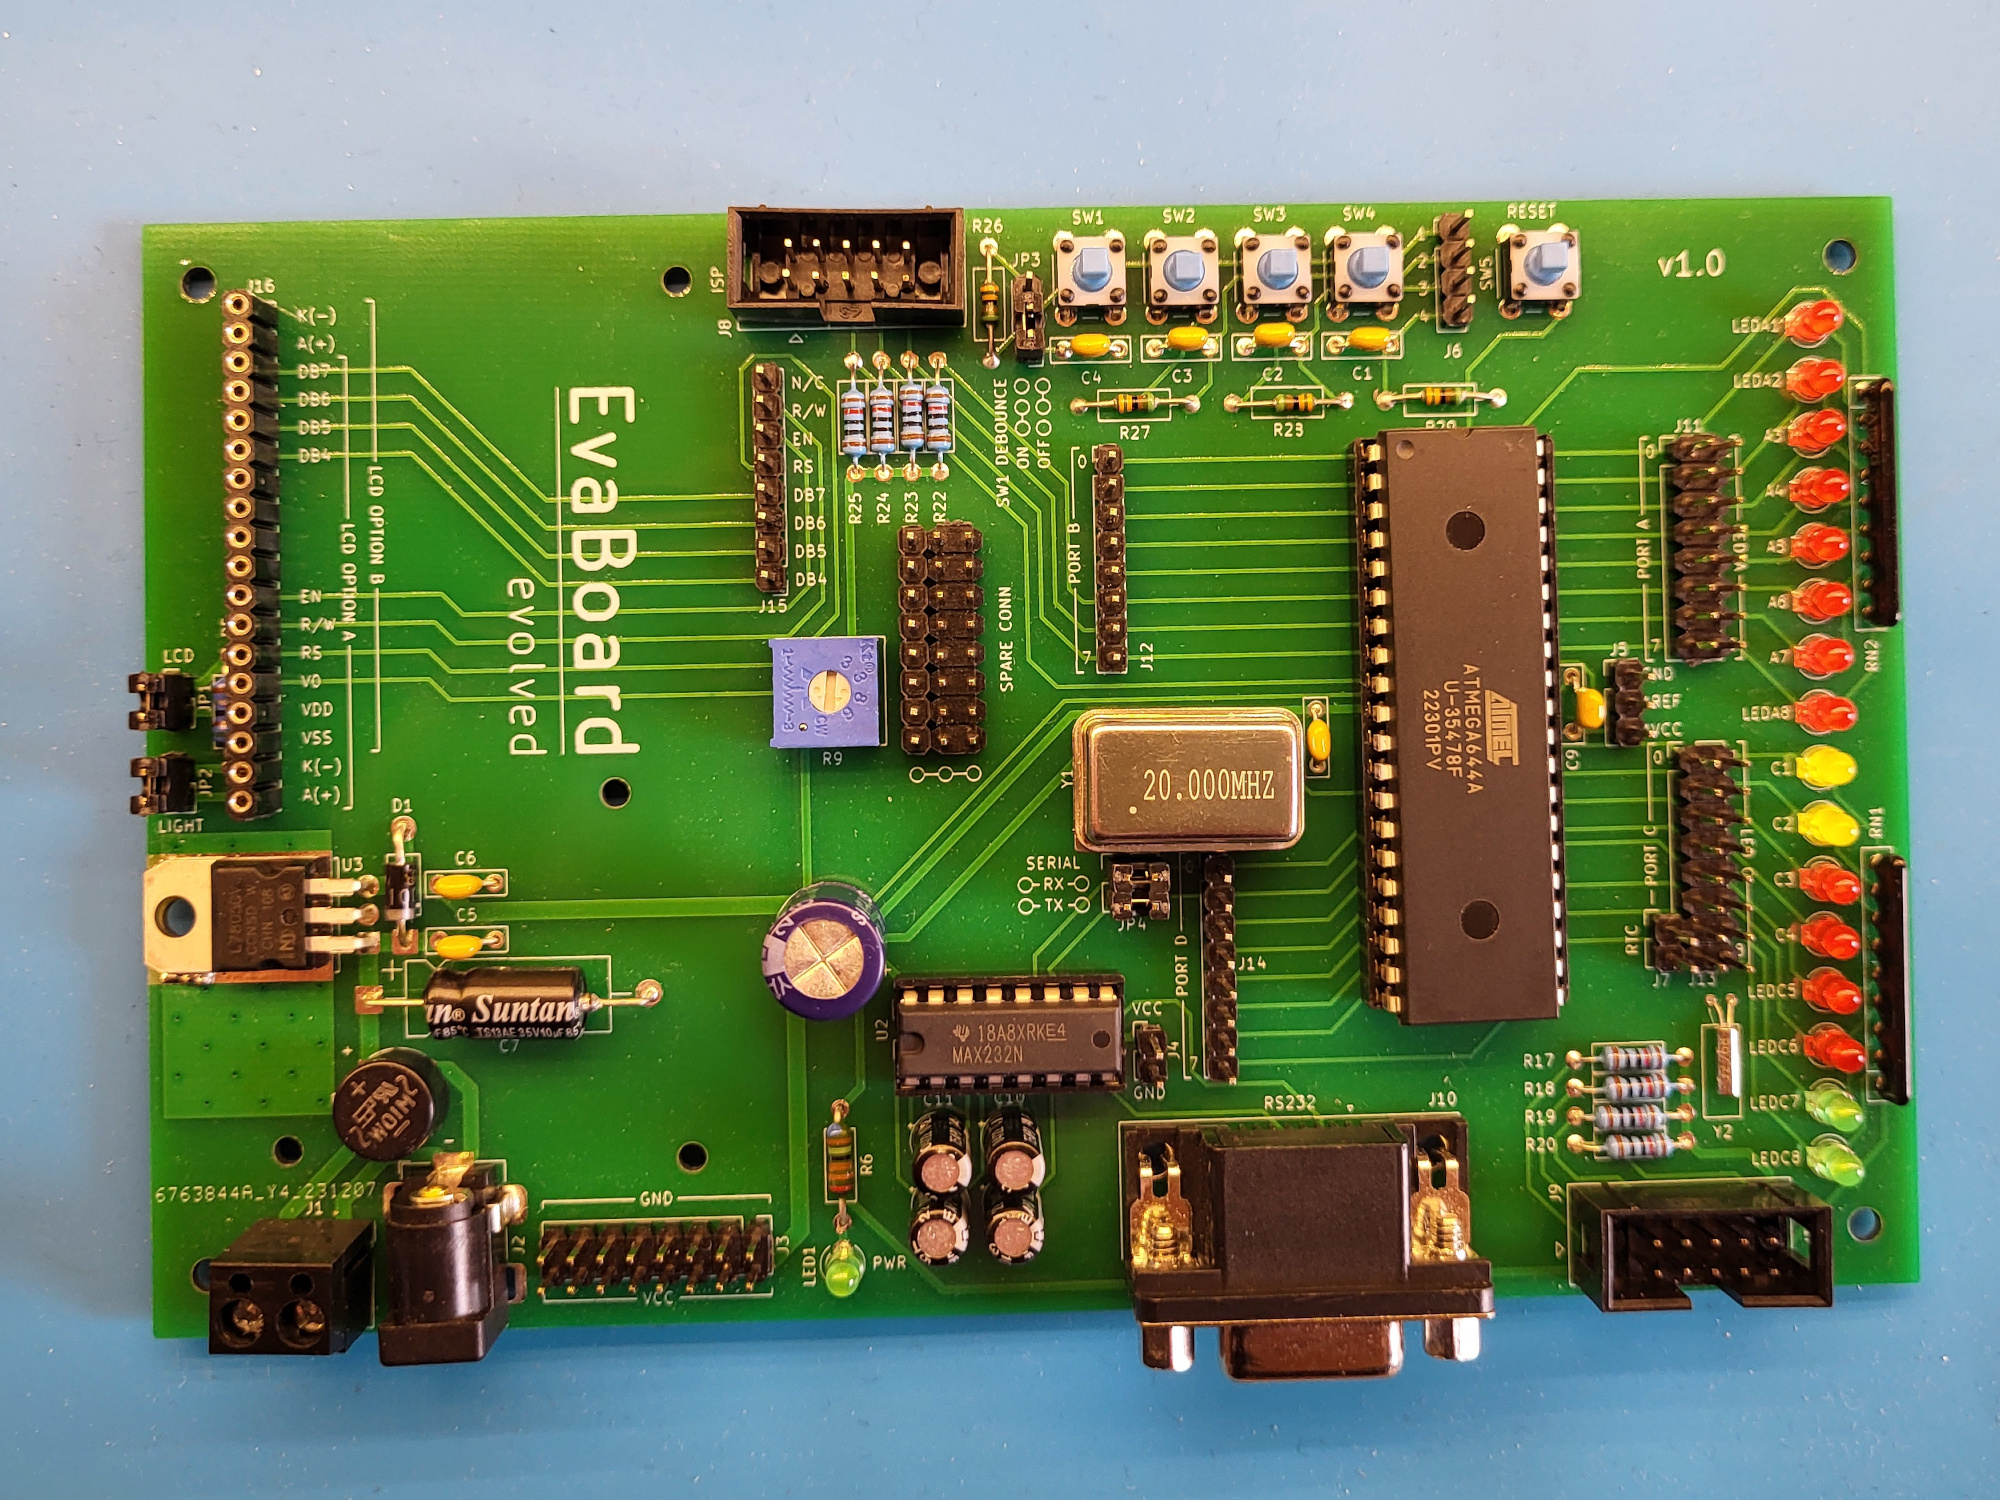
\includegraphics[width=0.85\textwidth]{Pictures/Finished.jpg}
\caption{The finished board}
\label{fig:finished}
\end{figure}

Check VCC again. It should not drop significantly from before the ICs were inserted. If it does, unplug the power immediately and make sure the ICs are inserted the right way. 

Finally, you can check the charge pump voltages: On Pin 2 of U2 you should get something between 8V and 10V (set the range of the multimeter accordingly). Pin 6 should have roughly the same voltage but negative. 

\section{Writing Firmware}
\subsection{Compilers and IDEs}\label{sec:compilersIDEs}
Making firmware for microcontrollers requires two pieces of software: a compiler that translates C code into machine code (or an assembler to translate assembly code into machine code) and a programmer software which copies the machine code to the microcontroller's flash with the help of a piece of hardware, confusingly also called a programmer. Integrated Development Environments (IDEs) are optional but simplify the process. 

Traditionally, \href{https://www.microchip.com/en-us/tools-resources/develop/microchip-studio}{Microchip Studio} was used to make firmware for ATmegas. This is an IDE that includes both a compiler and a programmer. It used to be called Atmel Studio before Atmel was purchased by Microchip. Microchip Studio is based on Visual Studio and thus runs only on Windows. It is quite old, missing many functions of modern IDEs and probably won't receive substantial updates since Microchip pushes its own IDE. 

\href{https://www.microchip.com/en-us/tools-resources/develop/mplab-x-ide}{MPLAB X} is the modern IDE by Microchip. It is based on NetBeans, runs on Windows, Linux, and macOS and receives regular updates. Originally intended for Microchip's own microcontroller series (``PIC''), it now supports all the Atmel ones as well, including ATmegas. Like Microchip Studio, it comes with a compiler (\href{https://www.microchip.com/en-us/tools-resources/develop/mplab-xc-compilers/xc8}{XC8}, to be downloaded separately) and a programmer which can be used through the IDE or as stand-alone software (MPLAB I\textbf{P}E). 

Finally, there is also open source software for ATmegas:
\begin{itemize}
\item \href{https://www.nongnu.org/avr/}{AVR-GCC}, a C compiler (this is actually the compiler that's included in Microchip Studio nowadays)
\item \href{https://github.com/Ro5bert/avra}{AVRA}, an assembler
\item \href{https://github.com/avrdudes/avrdude}{AVRDUDE}, a programmer software supporting many hardware programmers, both proprietary and open ones
\end{itemize}

Since these are all command line programs, they can be integrated into most IDEs (including Microchip Studio and MPLAB X which allows third-party programmers to be used through AVRDUDE). Some IDEs have pre-made plugins (e.g.\ AVR Eclipse plugin). 

\begin{note}
``AVR'' (probably from the inventors' initials) is the collective term used for several families of 8-bit microcontrollers. This includes the ATmega family, the ATtiny family, and many more. When searching for information online, the keyword ``AVR'' will probably bring up more useful results than ``ATmega''. 
\end{note}

\subsubsection{Example: Using AVR-GCC}\label{sec:exAvrGcc}
On Linux, installing AVR-GCC is as simple as installing three packages. For example on Ubuntu:
\begin{lstlisting}[language=bash]
sudo apt-get install gcc-avr avr-libc binutils-avr
\end{lstlisting}

For Windows, download\footnote{The toolchain is also part of Atmel Studio, so if you've installed the latter, you're all set.} the \href{https://www.microchip.com/en-us/tools-resources/develop/microchip-studio/gcc-compilers/}{AVR 8-bit Toolchain} from Microchip. Extract it somewhere and add the \file{bin} subdirectory to the PATH environment variable. 

Create a file \file{blink.c} with the contents from Listing \ref{lst:blink}. This is the microcontroller equivalent of ``Hello World'', a minimalistic program which flashes an LED connected to Port A0. 

\lstinputlisting[language=C,frame=single,label=lst:blink,caption=blink.c for AVR-GCC]{../Tests/Blink/blink.c}

Run the following commands:
\begin{lstlisting}[language=bash]
avr-gcc -DF_CPU=1000000 -Os -mmcu=atmega644 -o blink.elf blink.c
avr-objcopy -j .text -j .data -O ihex blink.elf blink.hex
\end{lstlisting}

The first command is the compiler and linker. The command line argument -Os tells the compiler to optimize for space and -mmcu identifies the microcontroller. The -D argument tells the compiler to define a global symbol \lstinline[language=C]{F_CPU} set to 1000000. This is the frequency in Hz and it is required by the \lstinline[language=C]{_delay_ms()} function. 

The second command turns the output of the linker (\file{blink.elf}) into Intel hex format (\file{blink.hex}) which most programmers take as input. 

\subsubsection{Example: Using Microchip Studio}\label{sec:exMchpStudio}
Microchip Studio is available for Windows only. Download it from the \href{https://www.microchip.com/en-us/tools-resources/develop/microchip-studio#Downloads}{Microchip website} and install it. During installation, you can uncheck everything except the AVR architecture. 

Click ``File'', ``New'', ``Project'', select ``GCC C Executable Project'', and enter ``Blink'' as the project name. Next, choose the ATmega644 or ATmega644A from the ATmega device family. 

The IDE will automatically create a main.c file with a main function template. Copy the contents of Listing \ref{lst:blink} into the file. Select the ``Release'' configuration from the dropdown below the menu bar. 

Right click on the ``Blink'' project in the Solution Explorer and go to ``Properties''. On the ``Toolchain'' page, go to ``AVR/GNU C Compiler'', ``Symbols'' and define a new symbol \texttt{F\_CPU=1000000}. 

Hit F7 to compile. The hex file is placed in the \file{Release} subdirectory of your project folder. See Figures \ref{fig:mchpStudio1}, \ref{fig:mchpStudio2}, \ref{fig:mchpStudio3}, and \ref{fig:mchpStudio4}. 

\begin{figure}[htb]
\centering
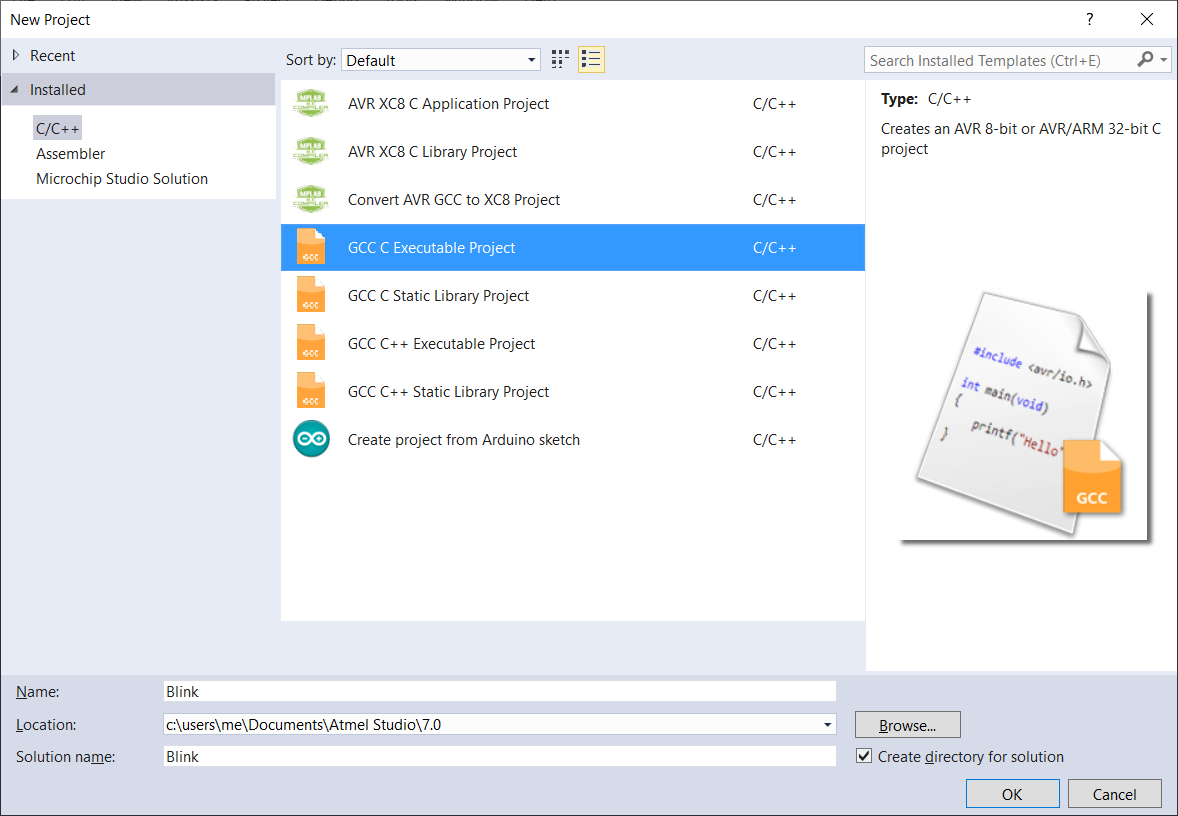
\includegraphics[width=0.6\textwidth]{Pictures/MchpStudio1.png}
\caption{Creating a New Project in Microchip Studio (Step 1)}
\label{fig:mchpStudio1}
\end{figure}

\begin{figure}[htb]
\centering
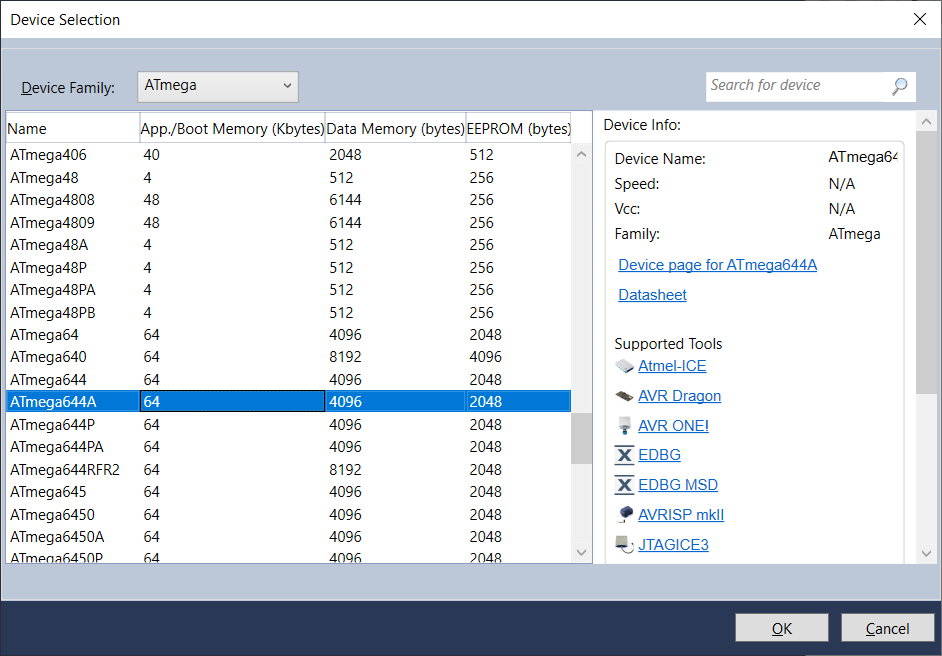
\includegraphics[width=0.6\textwidth]{Pictures/MchpStudio2.png}
\caption{Creating a New Project in Microchip Studio (Step 2)}
\label{fig:mchpStudio2}
\end{figure}

\begin{figure}[htb]
\centering
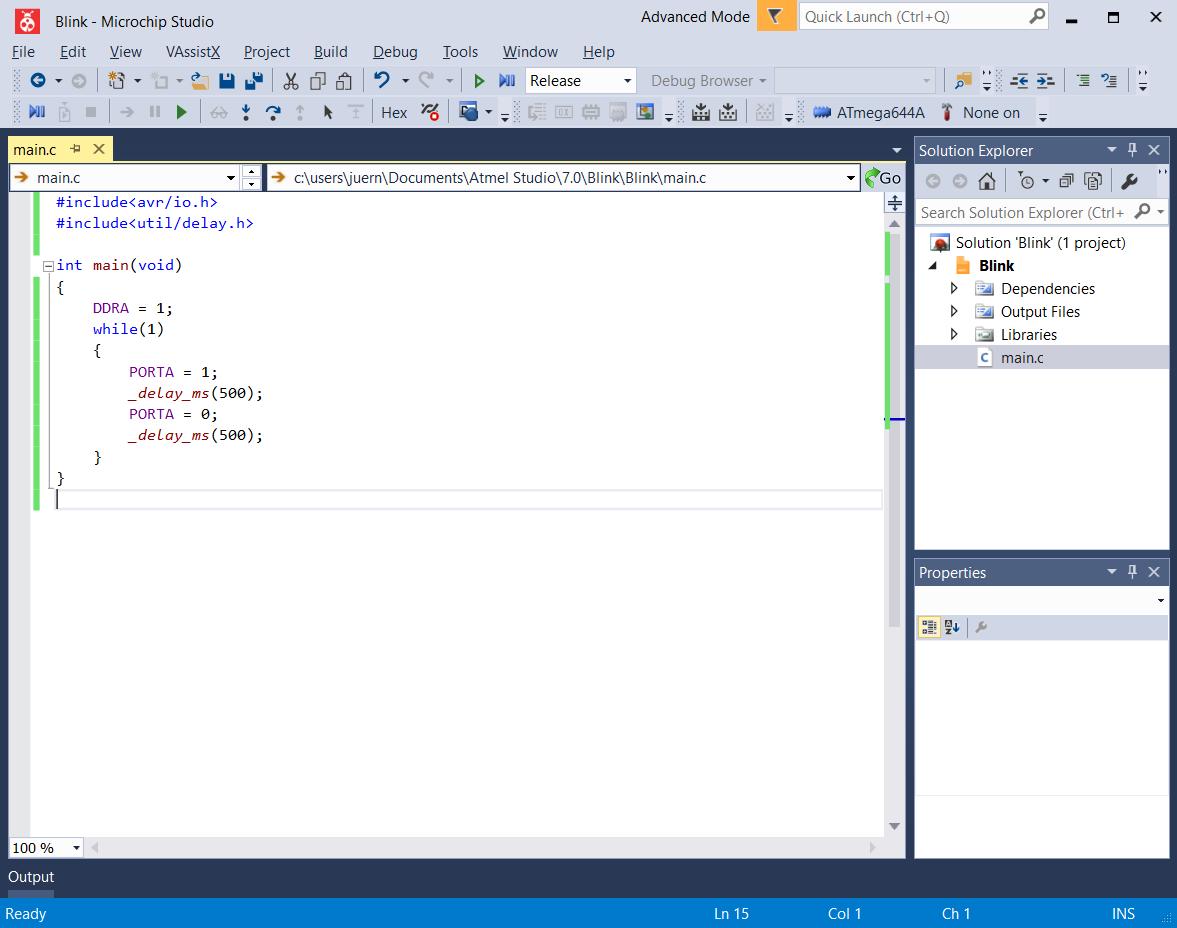
\includegraphics[width=0.8\textwidth]{Pictures/MchpStudio3.png}
\caption{Creating a New Project in Microchip Studio (Step 3)}
\label{fig:mchpStudio3}
\end{figure}

\begin{figure}[htb]
\centering
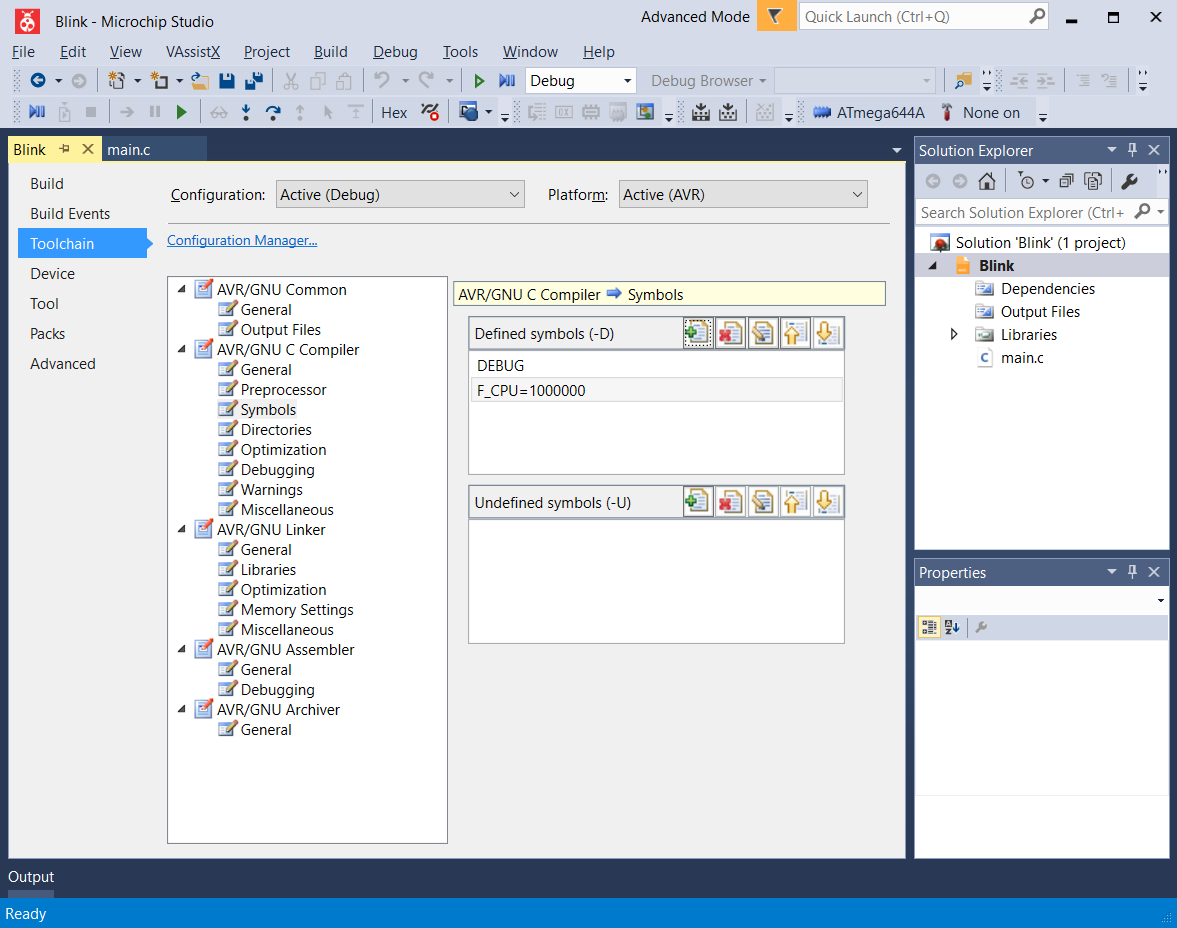
\includegraphics[width=0.8\textwidth]{Pictures/MchpStudio4.png}
\caption{Creating a New Project in Microchip Studio (Step 4)}
\label{fig:mchpStudio4}
\end{figure}
\FloatBarrier

\subsubsection{Example: Using MPLAB X}\label{sec:exMplabx}
Download MPLAB X from \href{https://www.microchip.com/en-us/tools-resources/develop/mplab-x-ide}{Microchip's website} and install it. On Windows, this is straightforward. On Linux, you have to unpack the installer, make it executable, and run it as root:
\begin{lstlisting}[language=bash]
tar xf MPLABX-vX.XX-linux-installer.tar
chmod u+x MPLABX-vX.XX-linux-installer.sh
sudo ./MPLABX-vX.XX-linux-installer.sh
\end{lstlisting}
The Linux installer places the software in \file{/opt/microchip/}. 

No compiler is included with the IDE, so you must choose which one(s) to install. One option is \href{https://www.microchip.com/en-us/tools-resources/develop/mplab-xc-compilers/xc8}{XC8}, Microchip's compiler for all its 8-bit microcontrollers. However, the free version of XC8 has some limitations when it comes to optimization. Another option is AVR-GCC which MPLAB X should automatically detect if it is installed (see Section \ref{sec:exAvrGcc} for how install it). From a programmer's perspective, both compilers work roughly the same. Refer to the \href{https://ww1.microchip.com/downloads/en/devicedoc/50002053g.pdf}{XC8 User's Guide} for details. 

Click ``File'', ``New Project'' and select ``Standalone Project'' from the ``Microchip Embedded'' category, then click ``Next''. Choose the ATmega644 or ATmega644A from the 8-bit AVR MCU category. If you are using an official Microchip programmer (see Section \ref{sec:programmers}), you can select it here, otherwise choose ``No Tool''. On the next screen, select XC8 or AVR-GCC as the compiler, whichever one you installed previously. Finally, name your project ``Blink'' and specify a location. Clicking ``Finish'' generates the project. See Figures \ref{fig:mplabx1}, \ref{fig:mplabx2}, \ref{fig:mplabx3}, and \ref{fig:mplabx4}. 

\begin{figure}[htb]
\centering
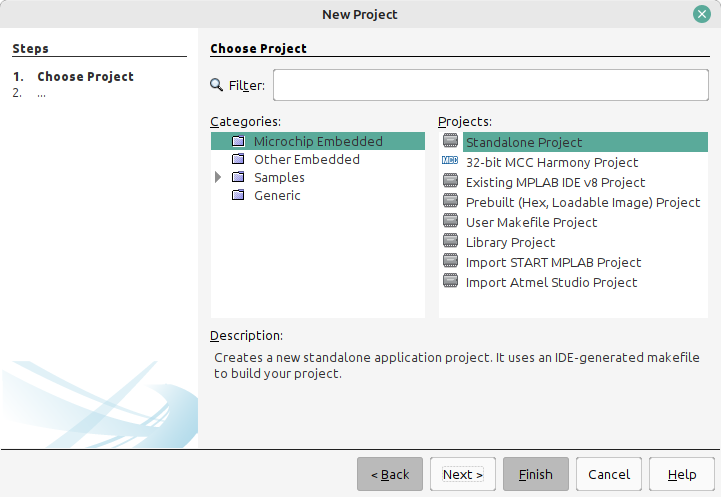
\includegraphics[width=0.6\textwidth]{Pictures/MPLABX1.png}
\caption{Creating a New Project in MPLAB X (Step 1)}
\label{fig:mplabx1}
\end{figure}

\begin{figure}[htb]
\centering
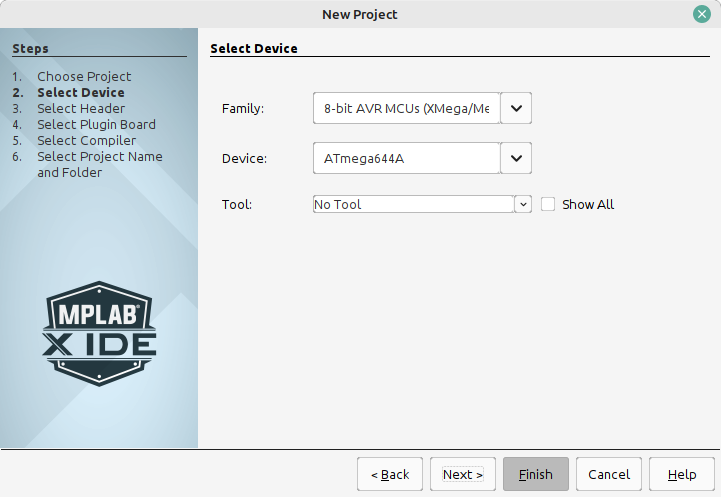
\includegraphics[width=0.6\textwidth]{Pictures/MPLABX2.png}
\caption{Creating a New Project in MPLAB X (Step 2)}
\label{fig:mplabx2}
\end{figure}

\begin{figure}[htb]
\centering
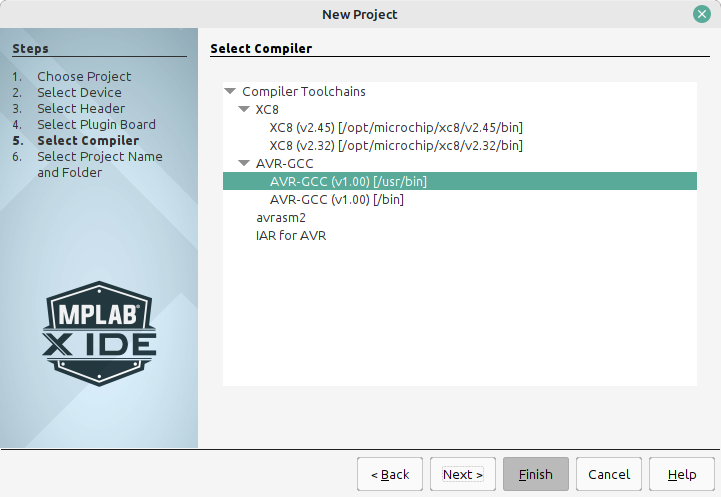
\includegraphics[width=0.6\textwidth]{Pictures/MPLABX3.png}
\caption{Creating a New Project in MPLAB X (Step 3)}
\label{fig:mplabx3}
\end{figure}

\begin{figure}[htb]
\centering
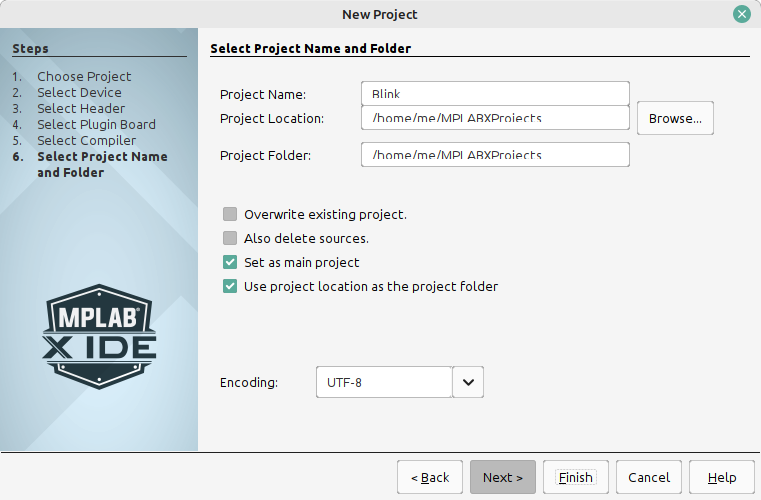
\includegraphics[width=0.6\textwidth]{Pictures/MPLABX4.png}
\caption{Creating a New Project in MPLAB X (Step 4)}
\label{fig:mplabx4}
\end{figure}

In the ``Project'' tab on the left-hand side, right click the ``Blink'' project and go to ``Properties''. On the compiler page (either ``avr-gcc'' or ``XC8 Compiler'') enter \texttt{-DF\_CPU=1000000} in the ``Additional options'' field and click ``OK''. See Figure \ref{fig:mplabx5}.  

\begin{figure}[htb]
\centering
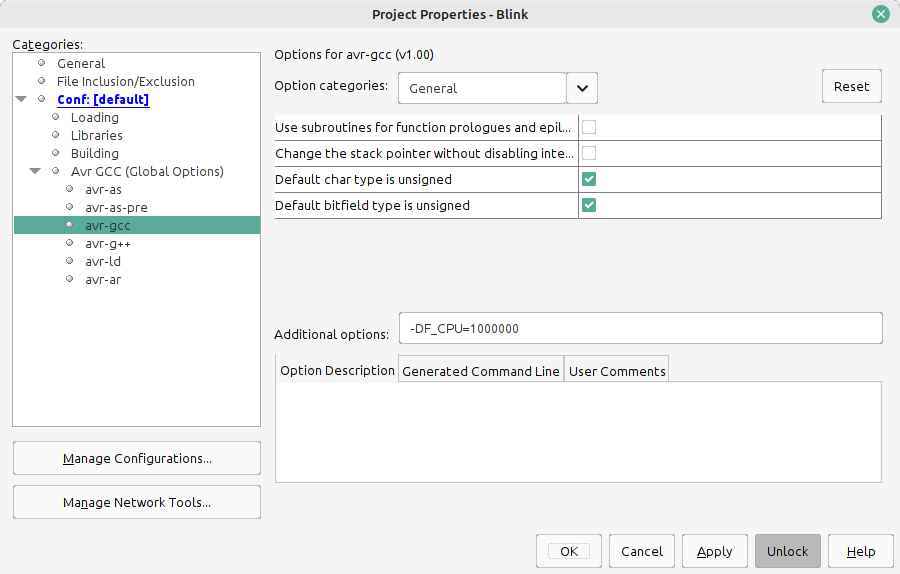
\includegraphics[width=0.6\textwidth]{Pictures/MPLABX5.png}
\caption{Creating a New Project in MPLAB X (Step 5)}
\label{fig:mplabx5}
\end{figure}

Right click ``Source Files'' in the ``Project'' tab and select ``New'', ``C Source File''. Enter ``blink'' as the file name and click ``Finish''. Enter the code from Listing \ref{lst:blink} into the empty file, like in Figure \ref{fig:mplabx6}. Press F11 to compile. MPLAB X places the hex file in the \file{dist/default/production} subdirectory of the project folder. 

\begin{figure}[htb]
\centering
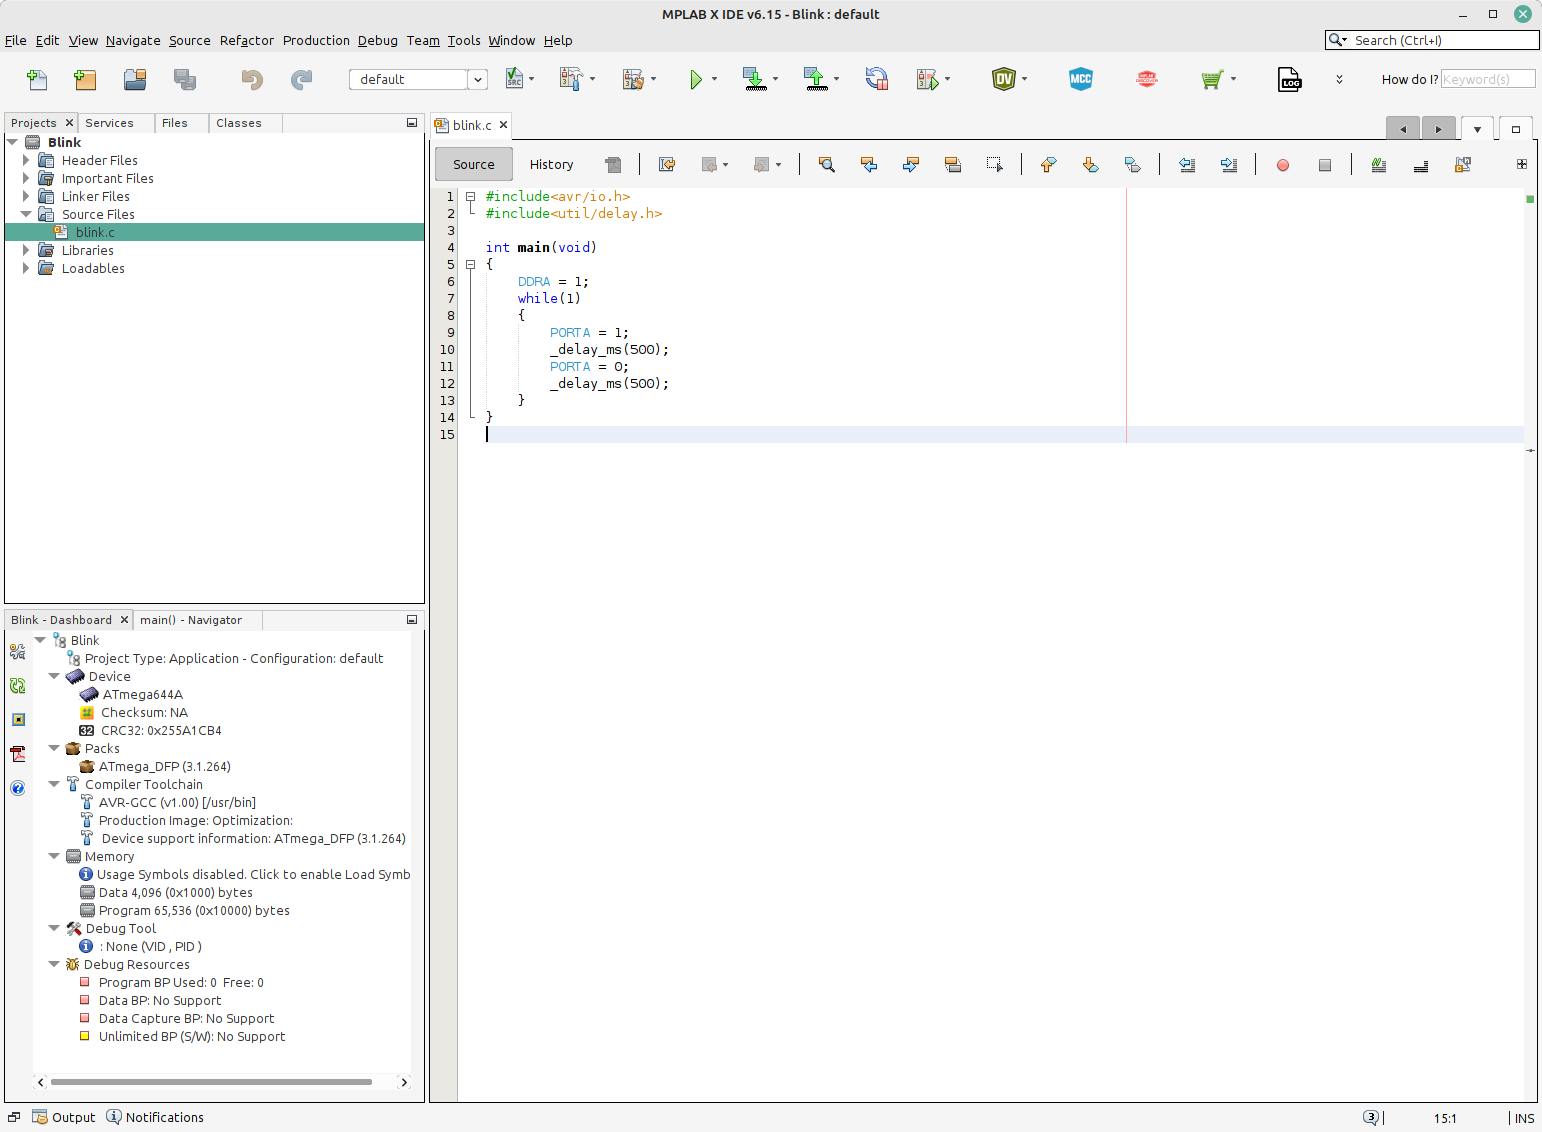
\includegraphics[width=\textwidth]{Pictures/MPLABX6.png}
\caption{Creating a New Project in MPLAB X (Step 6)}
\label{fig:mplabx6}
\end{figure}
\FloatBarrier

\subsection{Programmers and Debuggers}\label{sec:programmers}
In this context, ``Programming'' (or ``flashing'') means copying machine code from your PC to the program memory (flash) of the microcontroller. In addition to being programmed, the microcontroller can also be debugged, which means the computer can halt the microcontroller's execution and examine the contents of its memory and registers. A debugger is necessary for that. Debuggers can also act as programmers, so there's no need to switch back and forth. Programmers tend to be a lot cheaper than debuggers and have wider software support. 

The ATmega644(A) has two interfaces for programming: ISP and JTAG (connectors J8 and J9 on the board). JTAG can also be used for debugging, whereas ISP cannot. 

There is a wide variety of ISP programmers available both from Microchip and third parties, including open source ones. Things to pay attention to when choosing a programmer: the connection to the computer (USB, serial, parallel port etc.), whether it provides power to the target microcontroller while programming (we don't want that since the board has its own power supply), and what programming software supports it. 

\begin{itemize}
\item The \href{https://www.microchip.com/en-us/development-tool/atstk500}{STK500} is a rather dated programmer by Atmel which supports all ATmegas. It uses a serial connection to the PC and can provide power to the target (optional and with configurable voltage). It is supported by Microchip Studio and AVRDUDE. While it costs over 100\euro, there is a market for used ones. Its \href{http://atmel-studio-doc.s3-website-us-east-1.amazonaws.com/webhelp/GUID-D5634D24-82FD-4396-A28E-8A0F82B6FDE5-en-US-1/index.html}{schematic} and \href{https://www.microchip.com/content/dam/mchp/documents/OTH/ApplicationNotes/ApplicationNotes/doc2525.pdf}{communication protocol} are public. Some open source programmers are based on it and use the same protocol, although few offer the full range of functions of the STK500. \\
To some extend, the STK500 can itself be used as an evaluation board: It has sockets for different AVR microcontrollers, LEDs, buttons, and a serial port (but no LCD). \\
Despite its age, the STK500 comes with one major benefit: In addition to ISP, it is capable of high-voltage programming (HVP). For HVP, the microcontroller must be removed from the board and placed onto the STK500 (ISP stands for ``in system programming'' and HVP is not ``in system''). HVP works even if the microcontroller is bricked due to wrong fuse settings. See Section \ref{sec:fuses} for more details on fuses. 
\item The \href{https://www.microchip.com/en-us/development-tool/atavrisp2}{AVRISP mkII} is slightly newer and features a USB port. It provides no target power and is supported by Microchip Studio and AVRDUDE. It uses a 6-pin rather than a 10-pin connector, so you will need an adapter (some male-to-female jumper wires will also do). \\
The AVRISP mkII is no longer in production, but many clones are available, ranging from 20\euro{} to 30\euro. Some even come with an additional 10-pin header. 
\item One of the cheapest (and open source) options is \href{https://www.fischl.de/usbasp/}{USBasp}. You can get one for less than 5\euro{} on eBay or similar marketplaces. It uses USB1.1 low-speed (don't worry, your computer's USB2.0 is downward-compatible) and usually comes with a 10-pole ribbon cable that fits into the ISP connector (J8) of the evaluation board. The available models differ slightly, depending on the manufacturer. Make sure to choose one that lets you disable target power. Most have a three-pin (two-way) jumper for setting the target voltage to 5V (jumper right), 3.3V (jumper left) or off (no jumper). USBasp is supported by AVRDUDE. 
\begin{caution}
Do not buy the ``USBasp'' model that comes in a coloured metal case (sometimes with fraudulent Atmel branding). Those are not in fact USBasp clones and they don't work with AVRDUDE. 
\end{caution}
\item \href{https://www.arduino.cc/}{Arduino} is a popular microcontroller platform for hobbyists. Arduino boards consist of a microcontroller (often an ATmega328P) and a USB-to-serial converter. The microcontroller has a bootloader which allows it to be programmed directly from USB without the need for separate programmer hardware. Some Arduinos can be turned into ISP programmers for other ATmegas (supported by AVRDUDE). Suitable Arduino boards like Uno or Nano are 10\euro{} to 20\euro. 
\item There are \href{https://www.mikrocontroller.net/articles/AVR_In_System_Programmer#Programmer-Varianten}{many other options}. Before purchasing, check which software a particular programmer is supported by. 
\end{itemize}

Debuggers are significantly more expensive:

\begin{itemize}
\item The cheapest one is probably the \href{https://www.microchip.com/en-us/development-tool/pg164100}{MPLAB SNAP} by Microchip at around 65\euro. It connects via USB, has both ISP and JTAG, cannot supply target power, and is supported by MPLAB X and Microchip Studio (newer versions of AVRDUDE can use it as a programmer). Being Microchip's most low budget product, it comes with no case and is sometimes a bit unstable (expect the occasional USB disconnect). You will need an adapter for the 10-pin header of the evaluation board or a couple of male-to-female jumper wires. 
\item More expensive products like \href{https://www.microchip.com/en-us/development-tool/pg164140}{PICkit} or \href{https://www.microchip.com/en-us/development-tool/dv164045}{ICD} are more stable and offer optional target power. Like the SNAP, they were made for Microchip's PIC series and AVR support is more like an afterthought (again, adapter or jumper wires necessary). They all work with MPLAB X, some with Microchip Studio, and a few are supported by AVRDUDE as programmer only. 
\item Atmel's original JTAG adapter was the now discontinued \href{https://www.microchip.com/en-us/development-tool/ATJTAGICE3}{JTAGICE3}. Caution: The predecessors (JTAGICE mkI and mkII) do not support the ATmega644(A). The only ICE adapter still in production is the \href{https://www.microchip.com/en-us/development-tool/atatmel-ice}{ATMEL-ICE} at 200\euro{} to 300\euro. Both JTAGICE3 and ATMEL-ICE are supported by Microchip Studio and MPLABX. AVRDUDE can use them as programmers. 
\end{itemize}

\begin{note}
We recommend that, as a beginner, you go with the cheapest available ISP programmer. Not only will that still get you pretty far, you also won't burn serious money, should you somehow manage to fry it. 

Not having a debugger is less problematic than you might think. Hardware debugging is different from software debugging and comes with serious limitations. For example, while a debugger can halt the ATmega, other connected ICs keep running. Debugging also tends to interfere with interrupts, making it hard to reproduce problems in a debugging environment. Often the easiest way to debug firmware is to insert print commands that write values of interest to the LCD or the serial port. 
\end{note}

Due to the many possible combinations of programming hardware and software, we cannot give detailed instructions for every single one of them. Instead, the following subsections will pick a few examples and explain for each one how to program the \file{blink.hex} file from Section \ref{sec:compilersIDEs} onto the microcontroller. 

Prepare the board by connecting Pin A0 to LEDA1 using a jumper or jumper wire. Apply power to the board.

\subsubsection{Example: Programming with USBasp and AVRDUDE}\label{sec:exUsbaspAvrdude}
Remove the target power jumper (see Figure \ref{fig:usbasp}) from the USBasp. Connect it to your computer via USB and to the board's ISP connector J8 with the ribbon cable. 

\begin{figure}[htb]
\centering
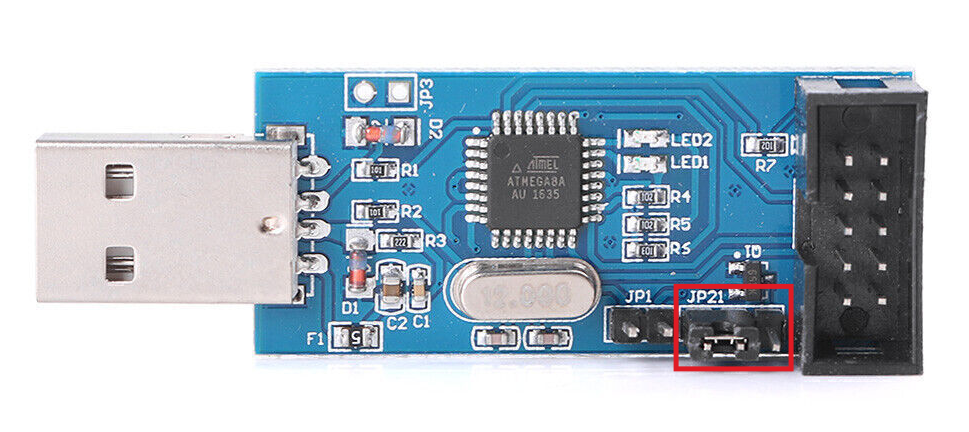
\includegraphics[width=0.6\textwidth]{Pictures/USBasp.png}
\caption{USBasp Programmer with Target Voltage Selection Jumper Highlighted}
\label{fig:usbasp}
\end{figure}

On Linux, all you have to do is install AVRDUDE via the package manager, e.g.\ on Ubuntu:
\begin{lstlisting}[language=bash]
sudo apt-get install avrdude
\end{lstlisting}

On Windows, USBasp will be listed as an unrecognised device in the Device Manager, like in Figure \ref{fig:deviceManagerBefore}. 
\begin{figure}[htb]
\centering
\frame{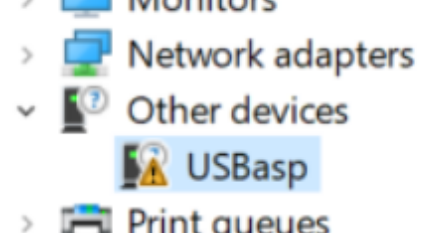
\includegraphics[width=0.4\textwidth]{Pictures/DeviceManagerBefore.png}}
\caption{Windows Device Manager before driver installation}
\label{fig:deviceManagerBefore}
\end{figure}

Download \href{https://zadig.akeo.ie/}{Zadig} and run it. Select USBasp and libusb as shown in Figure \ref{fig:driverUSBasp}, then hit ``Install Driver''. 
\begin{figure}[htb]
\centering
\frame{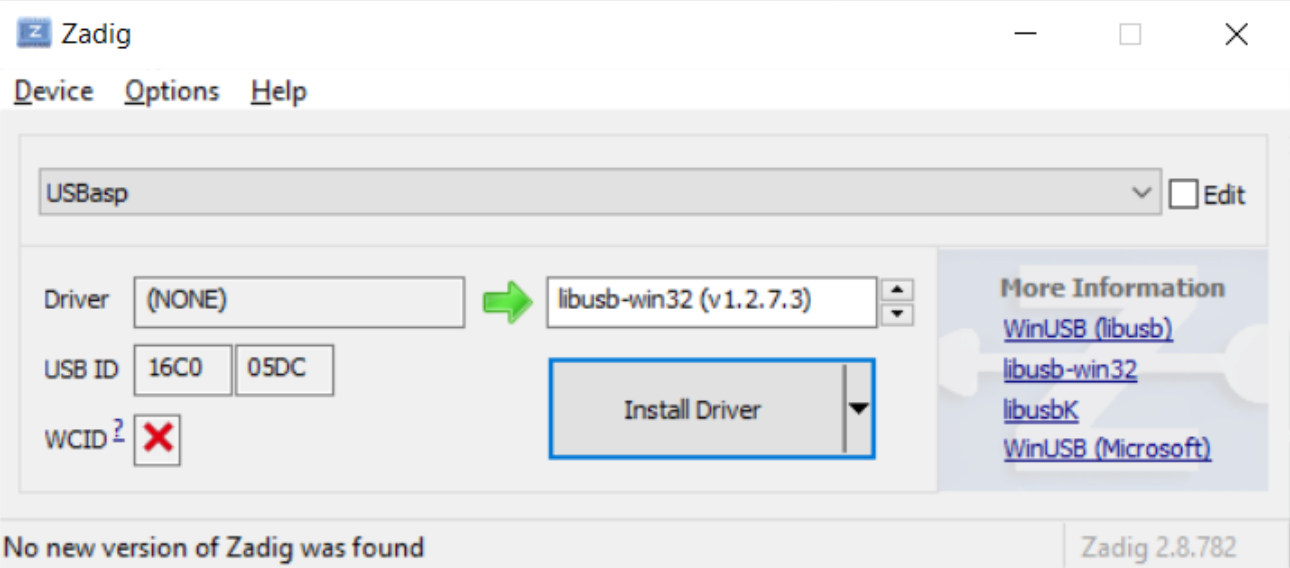
\includegraphics[width=0.85\textwidth]{Pictures/ZadigUSBasp.png}}
\caption{Install Windows Driver for USBasp}
\label{fig:driverUSBasp}
\end{figure}

Now the device manager should have USBasp as an ``Atmel USB Device'' like in Figure \ref{fig:deviceManagerAfter}. 
\begin{figure}[htb]
\centering
\frame{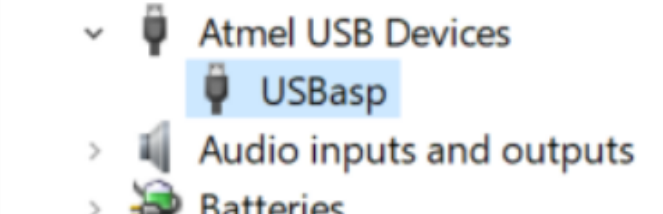
\includegraphics[width=0.4\textwidth]{Pictures/DeviceManagerAfter.png}}
\caption{Windows Device Manager after installation}
\label{fig:deviceManagerAfter}
\end{figure}

Next, download \href{https://github.com/avrdudes/avrdude/releases}{AVRDUDE} and unpack it somewhere (for example \file{C:\symbol{`\\}Program Files\symbol{`\\}avrdude}). In the system settings, add the directory to the PATH environment variable. Open a terminal window and type \lstinline[language=bash]{avrdude} to check whether Windows finds the program. 

On either platform, check if there is a connection to the ATmega:
\begin{lstlisting}[language=bash]
avrdude -c usbasp -p m644 -v
\end{lstlisting}

Change to the directory containing the \file{blink.hex} file, then flash it:
\begin{lstlisting}[language=bash]
avrdude -c usbasp -p m644 -U flash:w:blink.hex:i
\end{lstlisting}

If the LEDs starts blinking, you have successfully deployed your first microcontroller program. 

\subsubsection{Example: Programming with USBasp and Microchip Studio}\label{sec:exMchpStudioProg}
While Microchip Studio doesn't recognise third-party programmers directly, it can be configured to use AVRDUDE. First, make sure that AVRDUDE works from the command line, see Section \ref{sec:exUsbaspAvrdude}. 

\begin{enumerate}
\item Go to Tools \textrightarrow{} External Tools and add a new item 
\item As shown in Figure \ref{fig:microchipStudioUSBasp}, choose \file{avrdude.exe} for the command (in whichever directory you unpacked it). 
\item Set the arguments to
\begin{lstlisting}[language=bash]
-c usbasp -p m644 -U flash:w:$(ProjectDir)Release\$(TargetName).hex:i
\end{lstlisting}
\item There should now be a new item in the Tools menu. 
\end{enumerate}

\begin{figure}[htb]
\centering
\frame{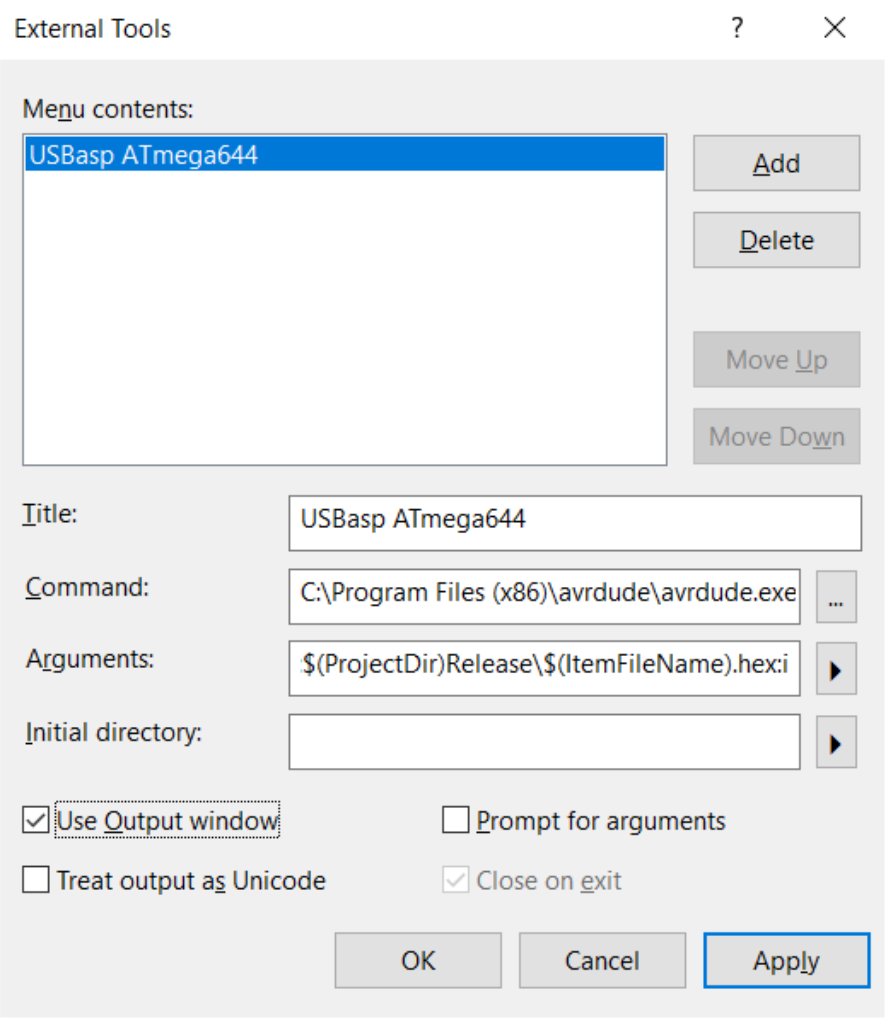
\includegraphics[width=0.6\textwidth]{Pictures/MicrochipStudioUSBasp.png}}
\caption{Adding a programming option for USBasp to Microchip Studio}
\label{fig:microchipStudioUSBasp}
\end{figure}

\begin{note}
In your projects, you have to select the ``Release'' target instead of ``Debug''. Or change the arguments accordingly. 
\end{note}

\subsubsection{Example: Programming with USBasp and MPLAB X}\label{sec:exMPLABX}
Like Microchip Studio, MPLAB X also doesn't recognise third-party programmers. There is no option to add a new menu item for an external tool, but you can specify a command to be executed after building. Unfortunately, this has to be done for every single project. 

AVRDUDE must be set up as described in Section \ref{sec:exUsbaspAvrdude}. 

Right-click on the project and go to ``Properties''. On the ``Building'' page, check ``Execute this line after build'' and enter
\begin{lstlisting}[language=bash]
avrdude -c usbasp -p m644 -U flash:w:${ImagePath}:i
\end{lstlisting}
into the text field. See Figure \ref{fig:AvrdudeMPLABX}. 

\begin{figure}[htb]
\centering
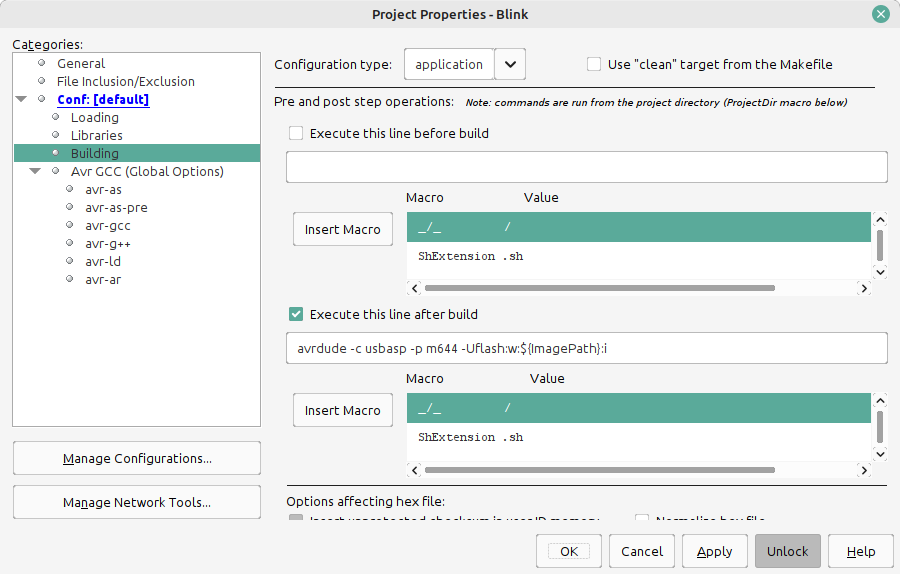
\includegraphics[width=0.8\textwidth]{Pictures/AvrdudeMPLABX.png}
\caption{Adding a programming option for USBasp to MPLAB X}
\label{fig:AvrdudeMPLABX}
\end{figure}

\FloatBarrier

\subsubsection{Example: Programming with Arduino and AVRDUDE}\label{sec:exArduino}
For this, you need an Arduino, a 10\textmu F capacitor, and some jumper wires. Several types of Arduino work, but it must be 5V tolerant. We recommend an Arduino Uno or Nano based on the ATmega328P. 

Install the \href{https://www.arduino.cc/en/software}{Arduino IDE} and connect the Arduino via USB. Your operating system should recognise the Arduino as a (virtual) serial port. The port is something like COM? on Windows or /dev/ttyUSB? on Linux, where the `?' is some number. 

From the ``Tools'' menu, select the board and processor you're using, as well as the port that the Arduino board is connected to, see Figure \ref{fig:arduinoIDE}. In the ``File'' menu, go to ``Examples'' and open ``ArduinoISP''. Click on the ``Upload'' button to program the Arduino. This is all the Arduino IDE is needed for, you can uninstall it now. 

\begin{figure}[htb]
\centering
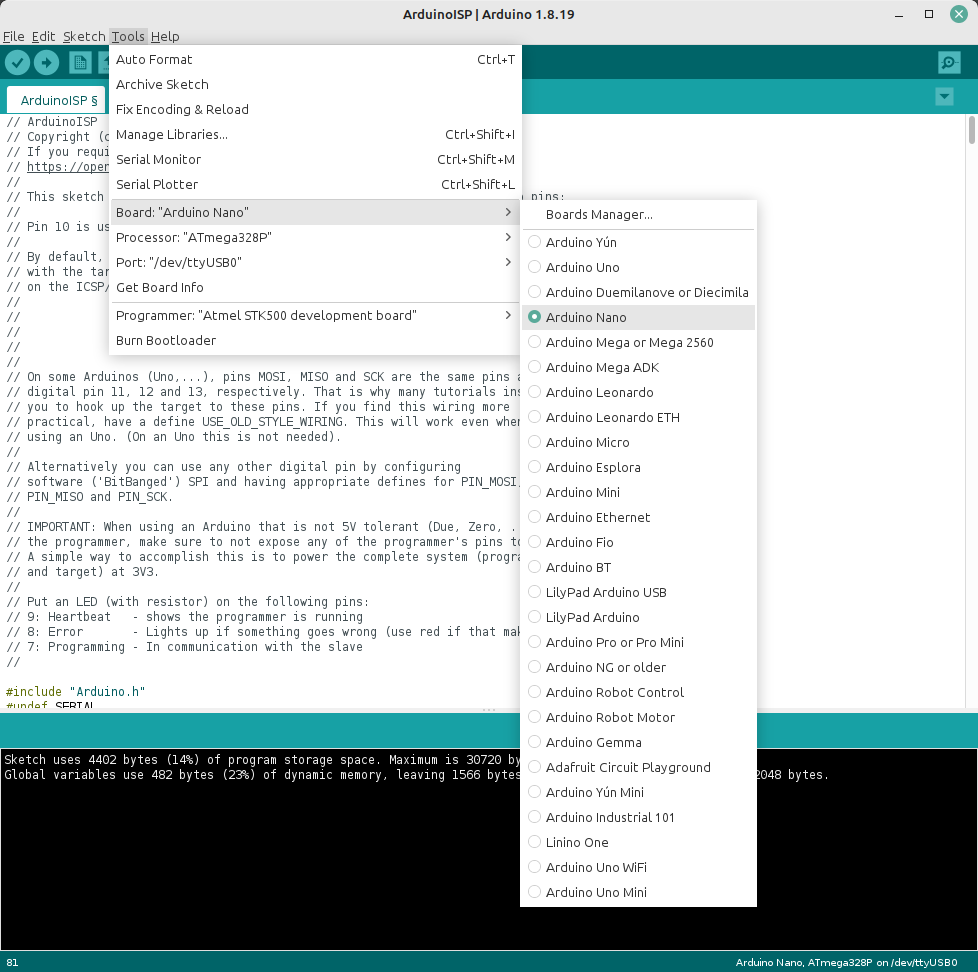
\includegraphics[width=0.8\textwidth]{Pictures/ArduinoIDE.png}
\caption{Programming an Arduino Nano to be an ISP Programmer}
\label{fig:arduinoIDE}
\end{figure}

Use five jumper wires to connect the Arduino to the evaluation board. They need to be male-to-female for the Uno and female-to-female for the Nano. Figure \ref{fig:arduinoISPConn} lists the necessary connections and shows the pins of the ISP connector J8. You also need to put a 10\textmu F capacitor between one of the Arduino's reset pins (``RST'') and GND. On the Uno, you can just stick it into the pin sockets. On the Nano, solder it to the pins or use female-to-female jumper cables. If you are using a polarised (electrolytic) capacitor, pay attention to the correct orientation. See Figure \ref{fig:arduinoProg} for an example. 

\begin{figure}[htb]
\begin{minipage}{.48\textwidth}
\centering
\begin{tabular}{l|l}
Arduino&ISP connector (J8)\cr\hline
D10&5 (RESET)\cr\hline
D11 (MOSI)&1 (MOSI)\cr\hline
D12 (MISO)&9 (MISO)\cr\hline
D13 (SCK)&7 (SCK)\cr\hline
GND&10 (GND)
\end{tabular}
\end{minipage}\hfill
\begin{minipage}{.48\textwidth}
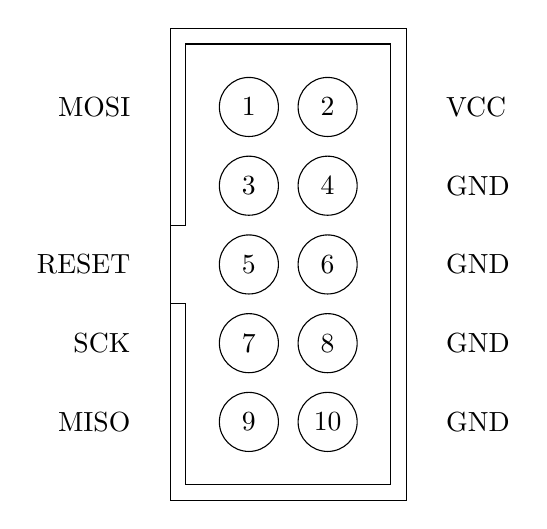
\begin{tikzpicture}[minimum size=0.75cm,label distance=1cm]
\node[draw,circle,label=left:MOSI] (1) at (0,5) {1};
\node[draw,circle,label=right:VCC] (2) at (1,5) {2};
\node[draw,circle] (3) at (0,4) {3};
\node[draw,circle,label=right:GND] (4) at (1,4) {4};
\node[draw,circle,label=left:RESET] (5) at (0,3) {5};
\node[draw,circle,label=right:GND] (6) at (1,3) {6};
\node[draw,circle,label=left:SCK] (7) at (0,2) {7};
\node[draw,circle,label=right:GND] (8) at (1,2) {8};
\node[draw,circle,label=left:MISO] (9) at (0,1) {9};
\node[draw,circle,label=right:GND] (10) at (1,1) {10};
\draw (-1,2.5) -- (-0.8,2.5) -- (-0.8,0.2) -- (1.8,0.2) -- (1.8,5.8) -- (-0.8,5.8) -- (-0.8,3.5) -- (-1,3.5);
\draw[draw] (-1,0) rectangle (2,6);
\end{tikzpicture}
\end{minipage}
\caption{Connections between the Arduino and J8 on the Evaluation Board}
\label{fig:arduinoISPConn}
\end{figure}

\begin{figure}[htb]
\centering
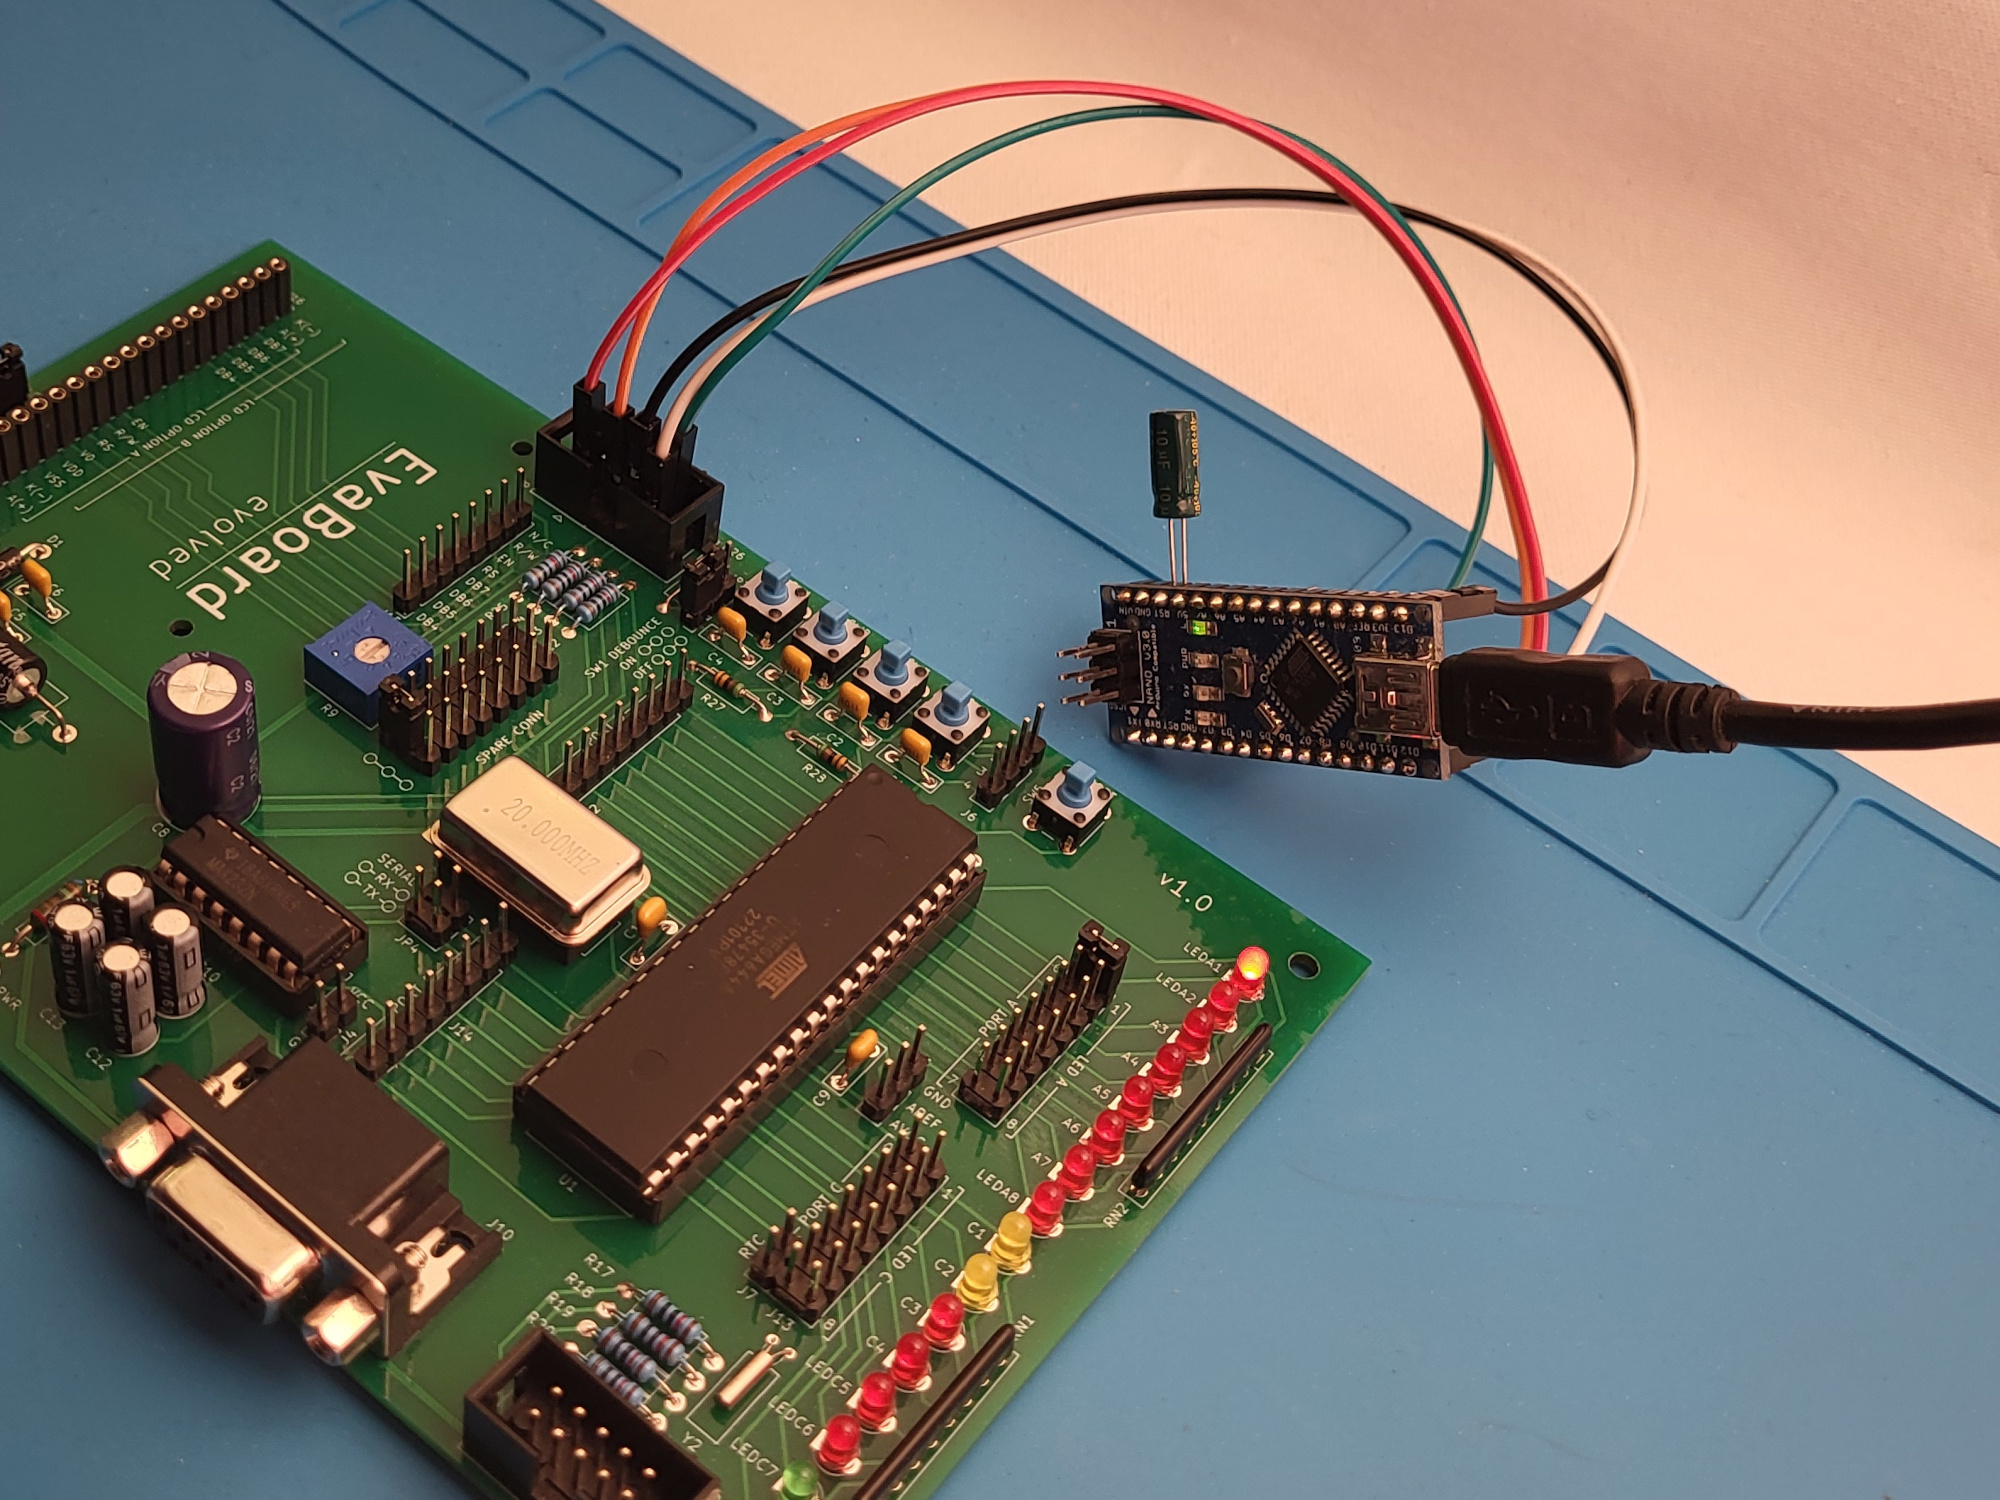
\includegraphics[width=0.85\textwidth]{Pictures/ArduinoProg.jpg}
\caption{Arduino Nano as ISP Programmer}
\label{fig:arduinoProg}
\end{figure}

Now you can program with AVRDUDE (insert the serial port after the \texttt{-P} argument):
\begin{lstlisting}[language=bash]
avrdude -c arduino -P <Serial Port> -b 19200 -p m644 -U flash:w:blink.hex:i
\end{lstlisting}

Just like in Sections \ref{sec:exMchpStudioProg} and \ref{sec:exMPLABX}, you can integrate AVRDUDE into your IDE. 
\FloatBarrier

\subsubsection{Example: Programming with STK500 and Microchip Studio}
The STK500 needs its own power supply. In theory you can power the evaluation board from the STK500, however, the amount of current the STK500 can provide to a target is limited. The better option is to have two power supplies, one for the STK500 and one for the evaluation board. In this case, you need to remove the VTARGET jumper, see Figure \ref{fig:stk500}. 

The STK500 requires a serial connection to the computer. If you are using a USB-to-serial converter, make sure it is properly recognised by Windows. Use the Device Manager to find out which COM port the STK500 is connected to. 

Use a 10-pole ribbon cable to connect ISP10PIN on the STK500 and the ISP connector (J8) on the evaluation board. Make sure to plug in the cable in the correct way -- the STK500 has Pin 1 labelled and on the evaluation board Pin 1 is marked with a small triangular arrow. 

\begin{figure}[htb]
\centering
\includegraphics[width=0.85\textwidth]{Pictures/STK500.png}
\caption{ISP Programming with STK500}
\label{fig:stk500}
\end{figure}

Start Microchip Studio and open the Blink project from Section \ref{sec:exMchpStudio}. In the ``Tools'' menu, click ``Add Target''. Select STK500 and specify the correct COM port, see Figure \ref{fig:stk500MchpStudio1}. Open the ``Device Programming'' dialog from the ``Tools'' menu. Select the STK500 entry in the Tool dropdown and make sure the ATmega644(A) is selected under ``Device'' and ISP under ``Interface''. Click ``Apply'', then have it read the device signature to check whether communication can be established. See Figure \ref{fig:stk500MchpStudio2}

\begin{figure}[htb]
\centering
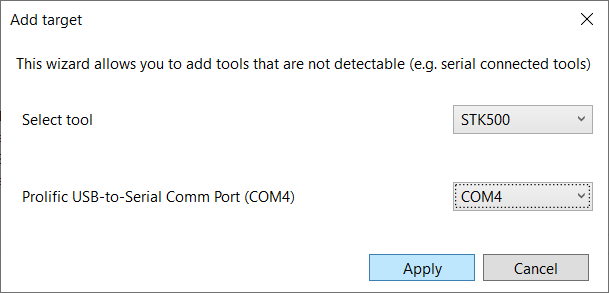
\includegraphics[width=0.65\textwidth]{Pictures/STK500MchpStudio1.png}
\caption{Adding the STK500 as a Target in Microchip Studio}
\label{fig:stk500MchpStudio1}
\end{figure}

\begin{figure}[htb]
\centering
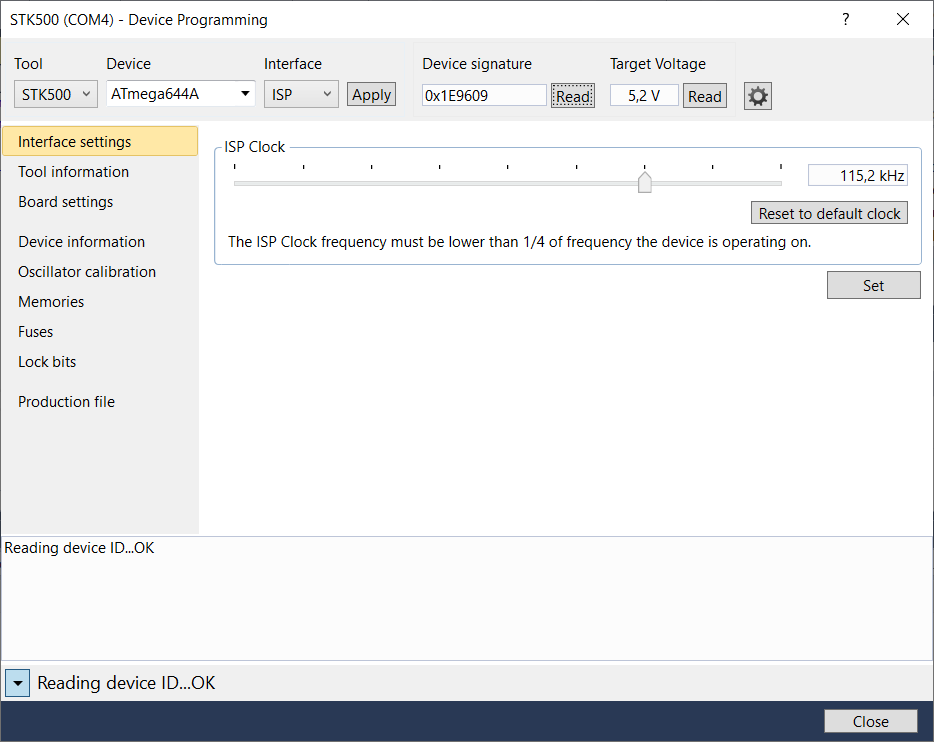
\includegraphics[width=0.85\textwidth]{Pictures/STK500MchpStudio2.png}
\caption{Settings for STK500 in Microchip Studio}
\label{fig:stk500MchpStudio2}
\end{figure}

In the project properties, go to the ``Tool'' page and select the STK500 and ISP, see Figure \ref{fig:stk500MchpStudio3}. Now you can program the microcontroller by clicking on the ``Start without Debugging'' icon in the toolbar, see Figure \ref{fig:stk500MchpStudio4}. 

\begin{figure}[htb]
\centering
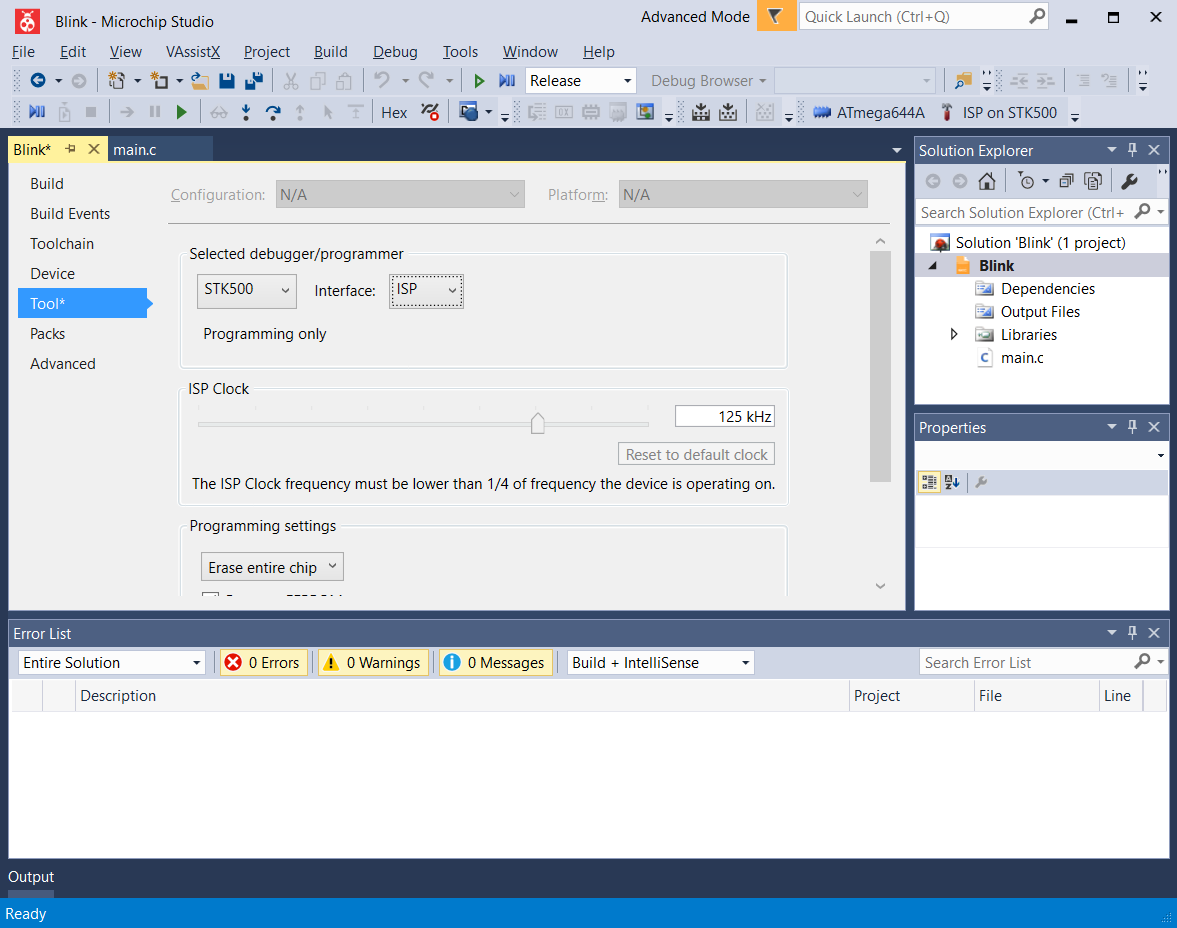
\includegraphics[width=0.8\textwidth]{Pictures/STK500MchpStudio3.png}
\caption{Project Settings for Programming with the STK500 in Microchip Studio}
\label{fig:stk500MchpStudio3}
\end{figure}

\begin{figure}[htb]
\centering
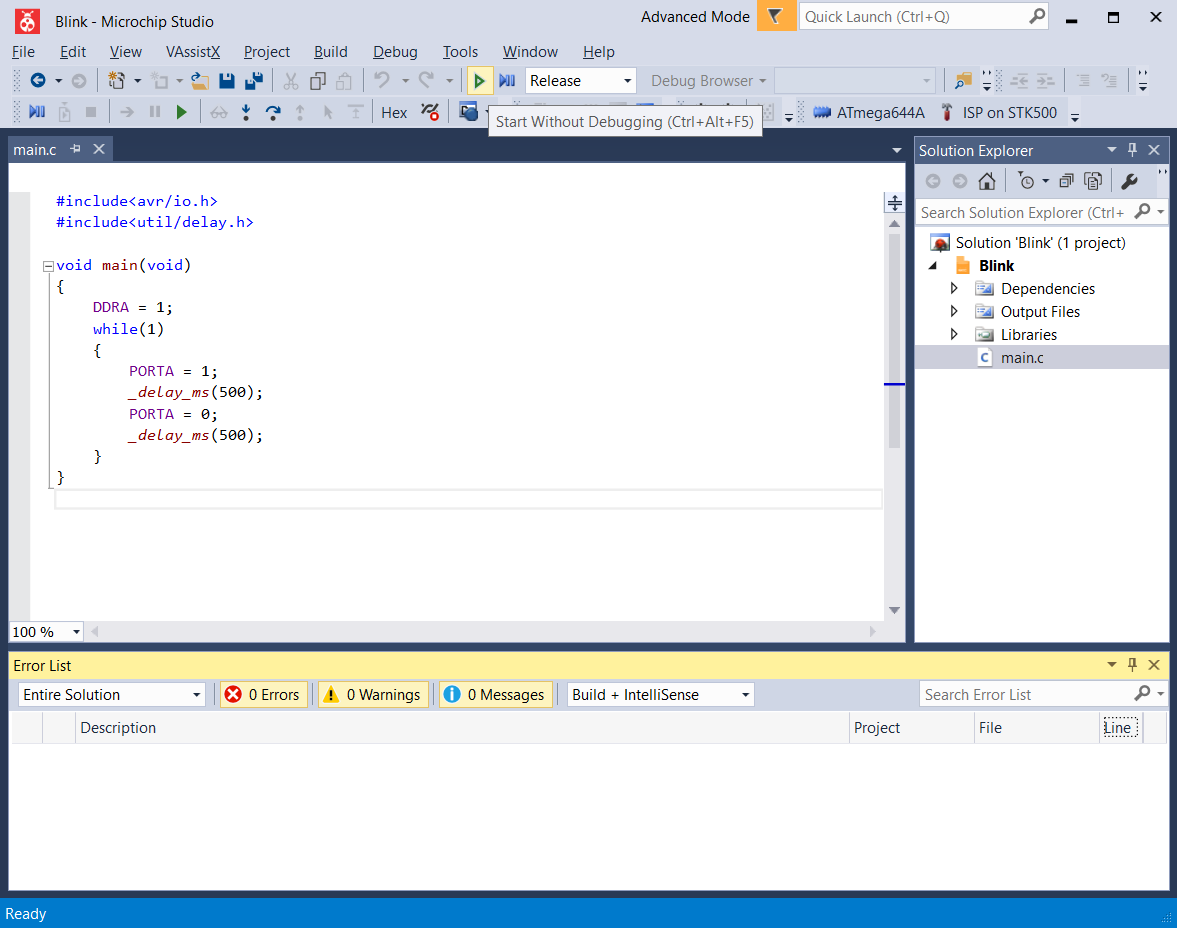
\includegraphics[width=0.8\textwidth]{Pictures/STK500MchpStudio4.png}
\caption{Programming with the STK500 in Microchip Studio}
\label{fig:stk500MchpStudio4}
\end{figure}
\FloatBarrier

\subsubsection{Example: Programming with MPLAB SNAP and MPLAB X}\label{sec:exSnap}
The SNAP supports both ISP and JTAG. In this example we are only looking at JTAG. 

The SNAP has an 8-pin socket to connect it to the target. The pin layout is made to fit standard programming connectors of PIC microcontrollers, so it cannnot be plugged directly into J9. Adapters from the 8-pin connector to the AVR JTAG 10-pin connector are available, but you can also just use seven male-to-female jumper cables. Figure \ref{fig:snapJTAGConn} lists the connections and shows the pin layout of the JTAG connector (J9). See also Table 10-4 of the \href{https://ww1.microchip.com/downloads/aemDocuments/documents/DEV/ProductDocuments/UserGuides/50002787C.pdf}{SNAP User's Guide}. Pins 1..8 on the SNAP are not individually labelled, but Pin 1 is marked by a small triangular arrow. 

\begin{caution}
The SNAP has a jumper that switches between ``AVR'' and ``PIC'', see Figure \ref{fig:snapJtag}. Make sure it is set in the ``AVR'' position. 
\end{caution}

\begin{figure}[htb]
\begin{minipage}{.48\textwidth}
\centering
\begin{tabular}{l|l}
MPLAB SNAP&JTAG connector (J9)\cr\hline
1 (TVPP)&--\cr\hline
2 (TVDD)&4 (VCC)\cr\hline
3 (GND)&2 (GND)\cr\hline
4 (PGD)&3 (TDO)\cr\hline
5 (PGC)&1 (TCK)\cr\hline
6 (TAUX)&6 (RESET)\cr\hline
7 (TTDI)&9 (TDI)\cr\hline
8 (TTMS)&5 (TMS)\cr\hline
\end{tabular}
\end{minipage}\hfill
\begin{minipage}{.48\textwidth}
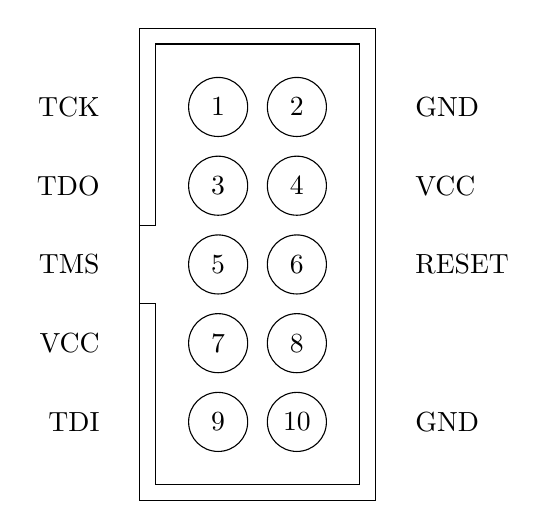
\begin{tikzpicture}[minimum size=0.75cm,label distance=1cm]
\node[draw,circle,label=left:TCK] (1) at (0,5) {1};
\node[draw,circle,label=right:GND] (2) at (1,5) {2};
\node[draw,circle,label=left:TDO] (3) at (0,4) {3};
\node[draw,circle,label=right:VCC] (4) at (1,4) {4};
\node[draw,circle,label=left:TMS] (5) at (0,3) {5};
\node[draw,circle,label=right:RESET] (6) at (1,3) {6};
\node[draw,circle,label=left:VCC] (7) at (0,2) {7};
\node[draw,circle] (8) at (1,2) {8};
\node[draw,circle,label=left:TDI] (9) at (0,1) {9};
\node[draw,circle,label=right:GND] (10) at (1,1) {10};
\draw (-1,2.5) -- (-0.8,2.5) -- (-0.8,0.2) -- (1.8,0.2) -- (1.8,5.8) -- (-0.8,5.8) -- (-0.8,3.5) -- (-1,3.5);
\draw[draw] (-1,0) rectangle (2,6);
\end{tikzpicture}
\end{minipage}
\caption{Connections between the MPLAB SNAP and J9 on the Evaluation Board}
\label{fig:snapJTAGConn}
\end{figure}

\begin{figure}[htb]
\centering
\includegraphics[width=0.85\textwidth]{Pictures/Snap.png}
\caption{MPLAB SNAP as JTAG Programmer}
\label{fig:snapJtag}
\end{figure}

Open the Blink project from Section \ref{sec:exMplabx} in MPLAB X. Open the project properties and on the ``Conf'' page, choose the SNAP from the tool dropdown. Once you hit ``Apply'', a new page named ``Snap'' appears. On it, go to the ``Communication'' category and make sure ``JTAG'' is the selected interface, see Figure \ref{fig:snapMplabX1}. Hit the ``Make and Program'' icon to start the programming, see Figure \ref{fig:snapMplabX2}. 

\begin{note}
The SNAP can be a bit fickle at times. If programming doesn't work, unplug and re-plug the USB cable. Try using a USB port directly on your computer rather than going through a USB hub. 
\end{note}

\begin{figure}[htb]
\centering
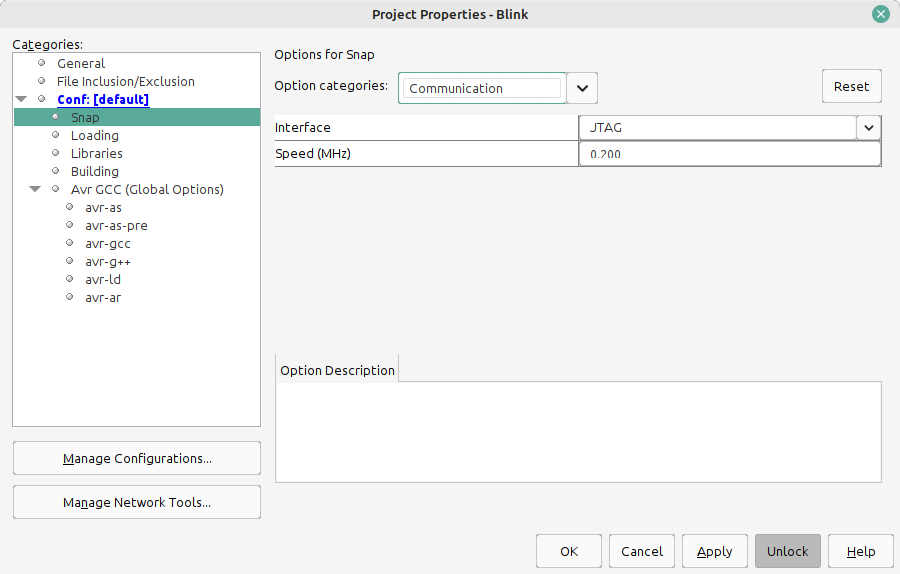
\includegraphics[width=0.85\textwidth]{Pictures/SNAPMPLABX1.png}
\caption{MPLAB X Settings for the SNAP}
\label{fig:snapMplabX1}
\end{figure}

\begin{figure}[htb]
\centering
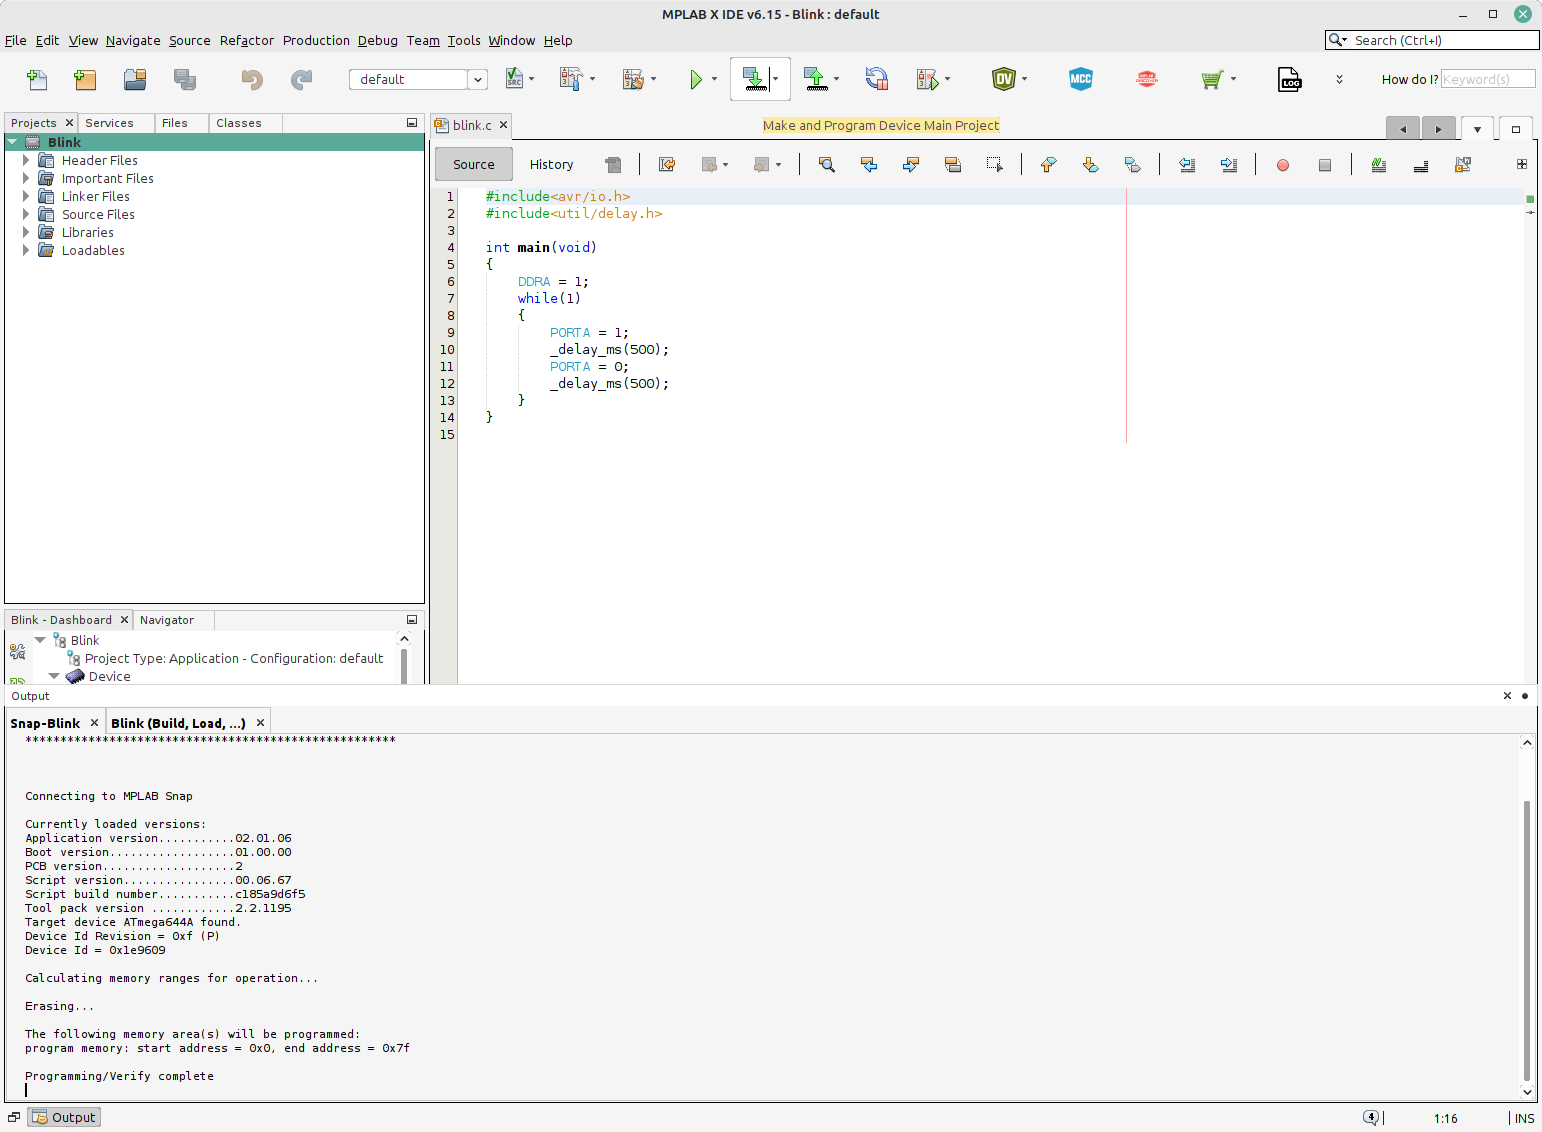
\includegraphics[width=\textwidth]{Pictures/SNAPMPLABX2.png}
\caption{Programming with the SNAP from MPLAB X}
\label{fig:snapMplabX2}
\end{figure}
\FloatBarrier

\subsection{Setting the Fuse Bits}\label{sec:fuses}
You might have noticed that, in the blink example, we told the compiler that the microcontroller's CPU frequency was 1MHz, not 20MHz. This is because, in its factory settings, the ATmega is configured to use the internal 8MHz clock generator and divide that clock by 8. In order to make it use the external crystal oscillator Y1 and not divide the clock, we need to change these settings, called ``fuse bits'' on the ATmega. 

\begin{caution}
Be very careful when doing this. Some fuse bits control the functioning of the programming pins. Setting them wrong can brick the microcontroller. When that happens, only high-voltage programmers (see Section \ref{sec:programmers}) can reset it. 
\end{caution}

For more details on the fuse bits, see Section 25.2 of the \datasheet. There are also online tools available, e.g.\ the \href{https://eleccelerator.com/fusecalc/fusecalc.php?chip=atmega644}{AVR Fuse Calculator}. For some reason the logic of the fuse bits is inverted. Note the weird language in the datasheet: it calls fuse bits ``programmed'' (meaning cleared, 0) and ``unprogrammed'' (meaning set, 1). 

We need to set (unprogram) Bit 7 (CKDIV8) of the low fuse byte and clear (program) Bit 1 (CKSEL1). This means changing the low fuse byte from its default value of 0x62 to 0xe0. 

In AVRDUDE this works as follows (using USBasp; similar for other programmers):
\begin{lstlisting}[language=bash]
avrdude -c usbasp -p m644 -u -U lfuse:w:0xe0:m
\end{lstlisting}

Both Microchip Studio and MPLAB X support setting fuses through a graphical user interface. However, this only works when using an officially supported programmer. Neither IDE can set the fuses via AVRDUDE. 

In Microchip Studio, open the ``Device Programming'' dialog from the ``Tools'' menu and go to the ``Fuses'' tab. Read the fuses, make the necessary changes, then write them back by clicking on the ``Program'' button. See Figure \ref{fig:mchpStudioFuses}. 

\begin{figure}[htb]
\centering
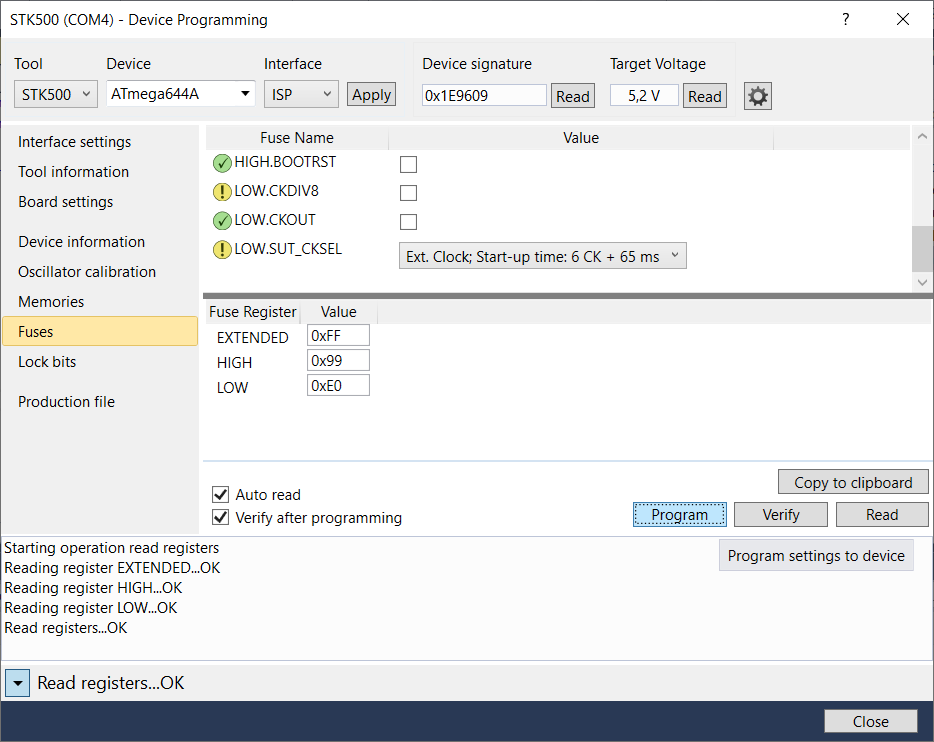
\includegraphics[width=0.65\textwidth]{Pictures/MchpStudioFuses.png}
\caption{Settings Fuses in Microchip Studio}
\label{fig:mchpStudioFuses}
\end{figure}

In MPLAB X, click ``Set Configuration Bits'' in the ``Production'' menu. First, click the ``Read Configuration Bits'' icon on the left. Make the necessary changes, then hit the ``Program Configuration Bits'' icon to write the modified values onto the chip. See Figure \ref{fig:mplabXFuses}. 

\begin{figure}[htb]
\centering
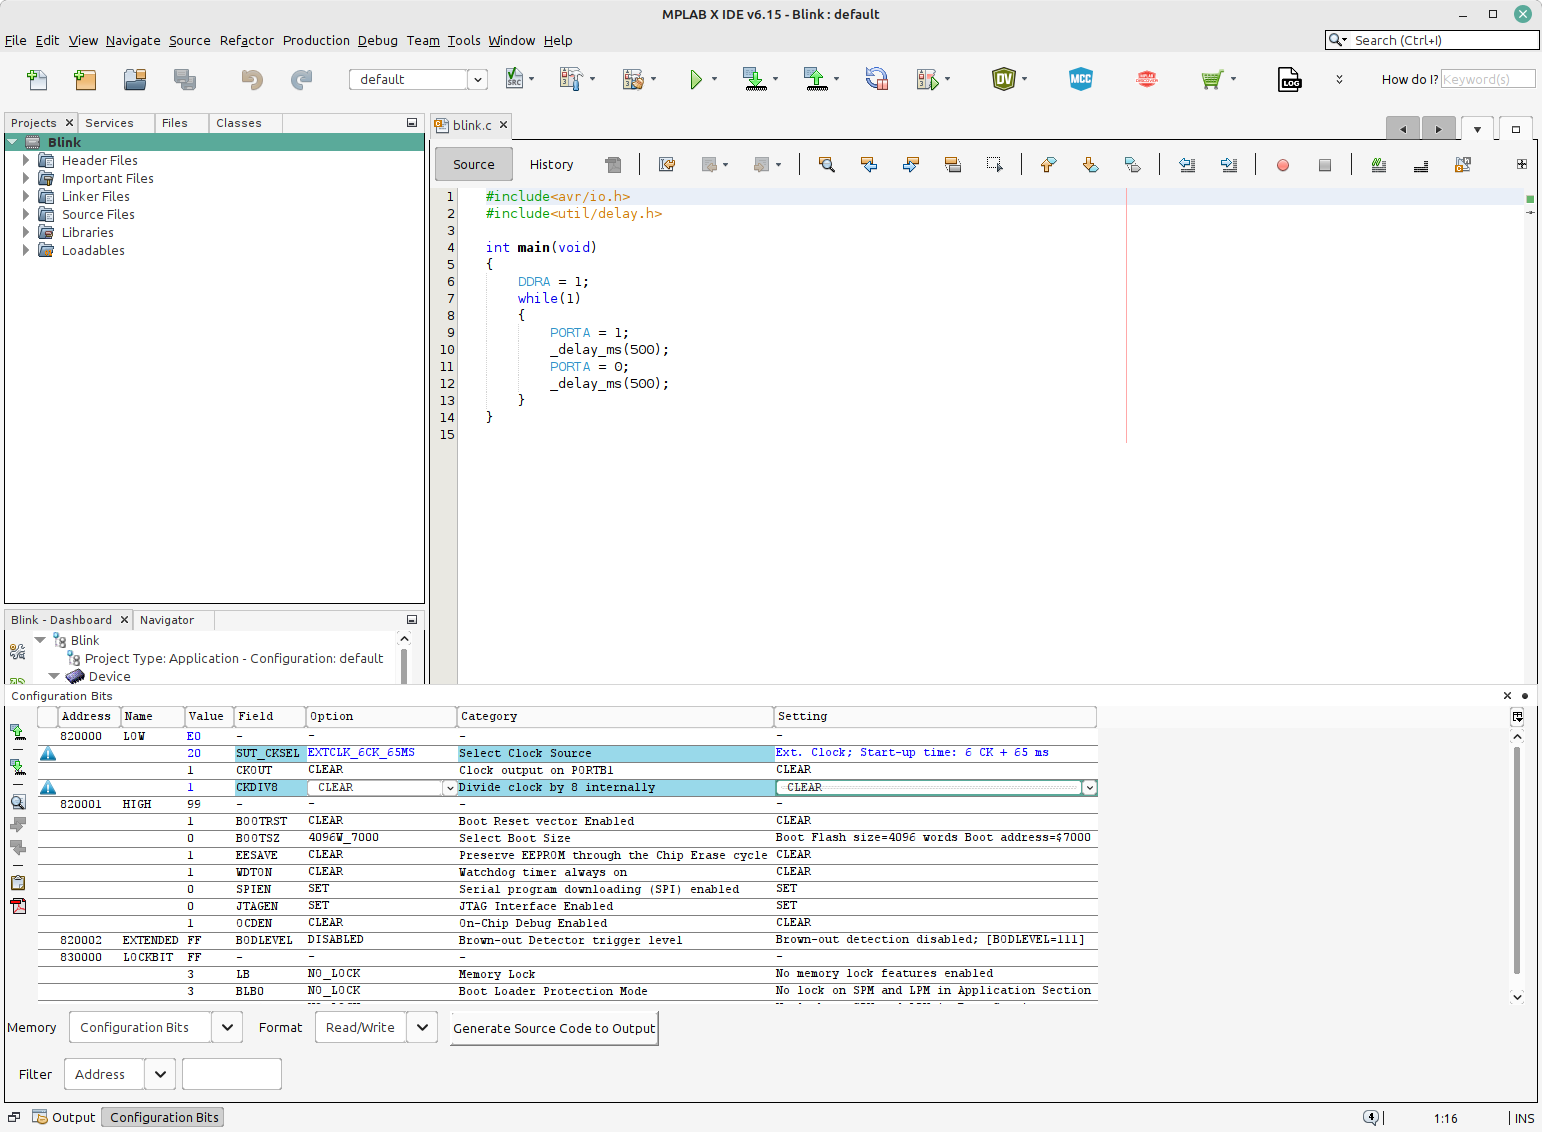
\includegraphics[width=\textwidth]{Pictures/MPLABXFuses.png}
\caption{Settings Fuses in MPLAB X}
\label{fig:mplabXFuses}
\end{figure}

The blink example should now flash 20 times faster. After re-compiling with the \lstinline[language=bash]{-DF_CPU=20000000} option, it should go back down to once per second. 
\FloatBarrier

\subsection{Testing (Part 2)}
Now that you are able to program the microcontroller, you can perform a full check of the hardware. 

The test programs can be found in the \href{../Tests/}{\file{Tests/} subdirectory} of this repository. They all come with makefiles for AVR-GCC, AVRDUDE, and USBasp. Modify the makefiles if you're using a different programmer. Alternatively, you can create a project in your IDE of choice and import the source files there. Be sure to define the \lstinline[language=C]{F_CPU} constant if your IDE doesn't do that automatically.

\begin{caution}
Be careful when switching from one project to the next. Changing the wiring of the board while there is still some old firmware running on the controller (or vice versa) might cause a short that can destroy the controller or other components. For example, a pin might previously have been connected to an LED and was thus configured as an output, but now gets connected to a button. 

The safest way to start a new project is to disconnect all wires and jumpers from the board, then erase the controller, then re-wire and flash new firmware. In AVRDUDE, erasing can be done like this:
\begin{lstlisting}[language=bash]
avrdude -c usbasp -p m644 -e
\end{lstlisting}
In the erased state, all pins are by default configured as inputs without pull-up which is usually safe. 
\end{caution} 

\subsubsection{Testing the LCD}\label{sec:testLCD}
The code for this test can be found in \href{../Tests/LCD/}{\file{Tests/LCD/}}. 

\paragraph{Preparation}
Connect the LCD (J15) to Port A (J11). Table \ref{tab:connLCD} lists the individual connection that need to be made. Figure \ref{fig:wiringLCD} shows the setup. 

\begin{table}
\centering
\begin{tabular}{r|l}
\textbf{LCD (J15)}&\textbf{Port A (J11)}\cr\hline
R/W&A6\cr\hline
EN&A5\cr\hline
RS&A4\cr\hline
DB7&A3\cr\hline
DB6&A2\cr\hline
DB5&A1\cr\hline
DB4&A0
\end{tabular}
\caption{Connecting the LCD to Port A of the ATmega}
\label{tab:connLCD}
\end{table}

\begin{figure}[htb]
\centering
\includegraphics[width=0.85\textwidth]{Pictures/WiringLCD.jpg}
\caption{Wiring for the LCD example}
\label{fig:wiringLCD}
\end{figure}

\paragraph{Expected Result}
The test program runs through several stages, testing most of the LCD driver's functions. When it is done, it shows the message ``\~{} Finished \~{}''. 

\paragraph{Troubleshooting}
Make sure the connections are correct and the jumpers JP1 (LCD) and JP2 (LIGHT) are set. Check the contrast voltage, as described in Section \ref{sec:testingHardware}. Unplug and re-plug the power after programming. 

Since timings are important, the microcontroller must be running at the correct speed. See Section \ref{sec:fuses} for how to verify this using the \texttt{blink} example. 

Many problems with the LCD stem from the fact that ``HD44780-compatible'' is not an actual fully specified standard. Therefore, such LCDs may exhibit subtle differences in behaviour. If nothing else works, try a different model. However, there is something else you can try first:

The LCD controller requires very specific timings: After each command from the microcontroller, it needs a pause to execute that command before it can receive the next one. The length of the pause depends on the kind of command, see Table 6 in the \href{https://cdn-shop.adafruit.com/datasheets/HD44780.pdf}{datasheet}. The LCD driver uses sufficiently long delays for LCDs that conform to the specification, but some clones might need longer pauses. 

There is an alternative to delaying: The data pins DB4..DB7 are actually bidirectional. When R/W is pulled high, the LCD will report its current status, including the ``busy flag'' which tells whether or not the execution of the last command has finished. Instead of waiting for a fixed time, the microcontroller can poll this flag. Uncomment \lstinline[language=C]{LCD_BUSY_TIMEOUT} in \file{lcd.h} to enable this functionality. 
If, on the other hand, you're not using busy flag polling, you can hard-wire R/W to GND, thus saving one microcontroller pin. 

\begin{note}
Some LCDs freeze when the microcontroller is being programmed and can only be reset by disconnecting the power. This is because during programming, the microcontroller is held in reset and all its pins are floating (they act as inputs with no pull-up). This might cause problems when it comes to the EN and R/W pins. \\
You can prevent this by adding two 100k\textOmega{} pull-down resistors from R/W and EN to GND. Don't use stronger pull-downs (i.e.\ smaller resistance values), otherwise the pull-downs start fighting with the 10k\textOmega{} external pull-ups that are connected to some of the ATmega's pins. Version 1.1 of the PCB already comes with spaces for such resistors (R30 and R31). In Version 1.0 you can solder them to the back side, see Figure \ref{fig:lcdPullDowns}. 
\end{note}

\begin{figure}[htb]
\centering
\includegraphics[width=0.85\textwidth]{Pictures/LCDPullDowns.jpg}
\caption{Adding external pull-down resistors to the LCD}
\label{fig:lcdPullDowns}
\end{figure}

\subsubsection{Testing the Serial Port}\label{sec:testSerial}
The code for this test can be found in \href{../Tests/Serial/}{\file{Tests/Serial/}}. 

\paragraph{Preparation}
Mount both jumpers on JP4 to connect the ATmega's RX and TX pins to the MAX232, see Figure \ref{fig:wiringSerial}. Use a serial cable or a USB-to-serial connector, to connect the board's serial port (J10) to your computer. 

\begin{figure}[htb]
\centering
\includegraphics[width=0.85\textwidth]{Pictures/WiringSerial.jpg}
\caption{Wiring for the Serial Example}
\label{fig:wiringSerial}
\end{figure}

Start a serial terminal program (for example \href{https://cutecom.sourceforge.net/}{CuteCom} on Linux or \href{https://www.putty.org/}{PuTTY} on Windows) and open a connection on the serial port using the following settings:
\begin{itemize}
\item Baud rate: 250000 (250kBaud)
\item 8 data bits, no parity, 1 stop bit (``8N1'')
\item No flow control
\end{itemize}

\paragraph{Expected Result}
After programming the controller, it should print a message to the serial terminal. After that, it will echo any text you send, with the vowels being cyclically shifted by one. 

\paragraph{Troubleshooting}
If it doesn't work, test the hardware starting from the computer's end. First, pull the serial cable from the board and instead connect Pins 2 and 3 with a jumper cable as shown in Figure \ref{fig:serialLoopback}. Now, the terminal should echo ever letter verbatim. If it doesn't, check whether you have opened the right serial port. On Windows, they are called \texttt{COM?} and on Linux either \file{/dev/ttyS?} or \file{/dev/ttyUSB?} with the `?' being replaced by a number. Try going through the numbers until you find the right one. 

\begin{figure}[htb]
\centering
\includegraphics[width=0.85\textwidth]{Pictures/SerialLoopback.jpg}
\caption{Loopback test with a USB-to-serial adapter}
\label{fig:serialLoopback}
\end{figure}

Note that USB-to-serial adapters will usually need a driver on Windows. Linux should recognize them out of the box. With some adapters there is an issue with Linux mistaking them for a braille reader. In this case, uninstall the \texttt{brltty} package. In order to access serial ports without root priviledges, the user must be added to the \texttt{dialout} group. 

Once the computer's serial port is working reliably, reconnect the cable to the board. Instead of the two horizontal jumpers on JP4, place just one vertically on the left two pins (see Figure \ref{fig:max232Loopback}). Again, this creates a loopback, this time involving the MAX232. If it doesn't work, it is an indication that something is wrong with the MAX232. Make sure the capacitors C10..13 have the correct polarity. Check the V+ and V- voltages as described in Section \ref{sec:testingHardware}. 
\begin{figure}[htb]
\centering
\includegraphics[width=0.85\textwidth]{Pictures/Max232Loopback.jpg}
\caption{Loopback test involving the MAX232}
\label{fig:max232Loopback}
\end{figure}

\paragraph{Serial debugging}
Once the serial port is working, it can be a great help when debugging firmware. Just copy \file{serial.c} and \file{serial.h} from the \href{../Drivers/Serial/}{\file{Drivers/Serial/} subdirectory} into your project, \#include the latter, and call \lstinline[language=C]{serialInit()} at the beginning of \lstinline[language=C]{main()}. After that you can use \lstinline[language=C]{printf()} to print variables, registers, and other useful information. 

\subsubsection{Testing the Watch Crystal}\label{sec:testY2}
The code for this test can be found in \href{../Tests/RTC/}{\file{Tests/RTC/}}. 

\paragraph{Preparation}
Connect the pins of J7 (RTC) to Port C6 and C7 (the lower left two pins of J13) using two jumpers. With another jumper, connect Port A0 to LEDA1 (the two top pins of J11). Finally, attach the LCD to J16 and connect J15 to J12 like in Table \ref{tab:connRTC}. See Figure \ref{fig:wiringRTC}. 

\begin{table}
\centering
\begin{tabular}{r|l}
\textbf{LCD (J15)}&\textbf{Port B (J12)}\cr\hline
R/W&B6\cr\hline
EN&B5\cr\hline
RS&B4\cr\hline
DB7&B3\cr\hline
DB6&B2\cr\hline
DB5&B1\cr\hline
DB4&B0
\end{tabular}
\caption{Connecting the LCD to Port B of the ATmega}
\label{tab:connRTC}
\end{table}

\begin{figure}[htb]
\centering
\includegraphics[width=0.85\textwidth]{Pictures/WiringRTC.jpg}
\caption{Wiring for the RTC example}
\label{fig:wiringRTC}
\end{figure}

\paragraph{Expected Result}
LEDA1 should blink in 1s intervals. After a short initial delay, the LCD should start displaying the current CPU frequency. 

\paragraph{Troubleshooting}
Apart from misplacing wires, not much can go wrong here. If it doesn't work, you have probably fried Y2 while soldering. 

\paragraph{Timers on the ATmega}
Besides testing the watch crystal Y2, this example illustrates working with timers. 
The watch crystal is used as an input for Timer 2. This is called ``asynchronous'' mode (as opposed to synchronous, where the a timer gets clocked by the CPU frequency). A 1:128 prescaler brings the frequency down from 32.768kHz to 256Hz. That means Timer2's counter TCNT2 increments 256 times per second. Since the counter uses 8 bits, it overflows once a second, producing an interrupt which switches LEDA1 on/off. 

We use another feature of Timer 2, the PWM generator. Typically, \href{https://en.wikipedia.org/wiki/Pulse-width_modulation}{PWM} is used for digital-to-analogue conversion. In this case, we set the threshold (register OCR2B) to 128. That way, every time the 8-bit counter reaches 128, the OC2B pin (Port D6) is set to zero, whereas each time the counter overflows it is set to 1. In other words, we will see a falling edge on that pin once every second, right in the middle between two overflow interrupts. We could have used this pin to drive the LED, but we will do something more interesting instead. 

In parallel to all this, Timer 1 runs at CPU clock speed. Even though Timer 1 is a 16-bit timer, it will overflow much more often, since its clock is so much faster (20MHz). Counting the number of Timer 1 overflows between two Timer 2 overflows would give us a rough estimate of the CPU frequency. For a more precise measurement, we also need to take note of the value of Timer 1's counter TCNT1 at the exact moment when Timer 2 overflows. We could do that in Timer 2's overflow interrupt service routine, but there is a more elegant way to do it in hardware: Timer 1 has a feature called ``input capture'' which stores TCNT1's value in a separate register ICR1 whenever there is a falling edge (or a rising one, this can be configured) on the ICP pin. As luck would have it, the ICP pin is Port D6, i.e.\ the exact same pin where Timer 2 produces a falling edge once every second. All that is left to do, is read ICR1 in the ICP interrupt service routine. The main program then calculates the CPU frequency from two consecutive ICR1 values and the number of Timer 1 overflows in between and shows it on the LCD. 

Note that this method relies on the accuracy of the watch crystal. The latter is not perfect -- its deviation is typically on the order of $\pm$20ppm (parts per million)\footnote{The error is mostly temperature-induced, as you can observe when carefully placing a finger on Y2. Higher quality RTC circuits auto-calibrate using temperature sensors. This brings the error down from $\pm$20ppm (10min/year) to less than $\pm$1ppm (30s/year)}. This is still better than the crystal oscillator Y1 ($\pm$100ppm), let alone the ATmega's internal oscillator ($\pm$10\%). In fact, an external watch crystal like Y2 could be used to calibrate the internal oscillator (see Section 7.12.1 of the \datasheet). 

\section{Advanced Topics}
\subsection{Use of the Programming Pins in Applications}
Some of the 32 GPIO pins of the ATmega are used for programming and debugging. We have to be careful when connecting these to other hardware. 

\begin{note}
In all the examples in this document, this has been taken into consideration. But other applications may not do so -- pay attention, especially when they use a different type of programmer than you do. 
\end{note}

This section only provides the very basics of sharing programming lines. For more detailed information, see Section 4 of the \href{https://ww1.microchip.com/downloads/en/appnotes/atmel-2521-avr-hardware-design-considerations_applicationnote_avr042.pdf}{AVR042} Application Note. 

\paragraph{ISP} ISP programming happens on Pins B5..B7 (and the reset pin). This does not mean, however, that you cannot use them for other things. But you need to make sure that whatever device is connected to the pins satifies the following conditions:
\begin{enumerate}
\item During programming, the device must be able to cope with arbitrary signals on these pins. 
\item During programming, the device must not interfere. First and foremost, it must not attempt to output anything. Second, it should not put a substantial load on these lines (like a large capacitance or other things that draw large currents or prevent fast switching), although this can sometimes be mitigated by choosing a slower programming speed. 
\end{enumerate}

LEDs are usually fine -- of course they flash during programming. Buttons (not pressed!) are also ok, even with weak (i.e.\ high \textOmega{} value) external pull-up or pull-down resistors. 

One thing you have to be very careful about is the LCD. This is because it outputs data on DB4..DB7 when R/W is high. The best solution is to connect the LCD to some port other than B when programming over ISP. 
If you insist on using Port B, make sure that either R/W is kept low (and you cannot do this via the microcontroller because it is in reset during programming!) or that DB4..DB7 are connected to pins other than B5..B7. This is one of the reasons why in most examples the LCD is connected ``twisted'', i.e.\ DB4..DB7 go to Pins B0..B3. 

After programming, when the ATmega is running, any well-behaved ISP programmer stops outputting on the ISP lines. Thus, you can leave it connected. 

\begin{note}
If you know about \href{https://en.wikipedia.org/wiki/Serial_Peripheral_Interface}{SPI} (perhaps from using the SRAM add-on board), you can actually understand ISP in a bit more detail. It is no coincidence that ``ISP'' is an anagram of ``SPI''. In fact, ISP uses the SPI protocol: The programmer acts as the SPI master and the ATmega as the SPI device. This explains why ISP uses the same MOSI, MISO, and SCK pins as SPI. The reset pin of the ATmega acts as CS. 

Remember that SPI devices leave the SPI lines alone when not selected. This means in particular, that any other SPI devices can stay connected during ISP programming, as long as their CS lines have pull-ups that keep them de-selected. The 23LC1024 on the SRAM add-on board is an example of this. 
\end{note}

\paragraph{JTAG} JTAG uses Pins C2..C5 (and the reset pin). If you are programming and debugging via JTAG, these pins are in use the whole time. Do not connect anything else to them. 

If you're only programming via JTAG but not debugging, the same conditions as with ISP apply. However...why would you be doing this? If you're not debugging anyway, just use ISP and save some pins. 

\paragraph{Other pins} While the ATmega is being programmed, it is held in reset. This means that all other pins are ``high impedance'' or ``floating'' (which essentially means they are configured as inputs without pull-up). In most cases, this is perfectly safe, regardless of what other devices are connected to them. Only some LCDs have an issue with floating pins, as we mentioned in Section \ref{sec:testLCD}. 

\subsection{Debugging}
On the surface, debugging a microcontroller program looks similar to ``normal'' debugging. You can set breakpoints, step through the code, and examine the contents of the memory. 

Internally though, hardware debugging is a bit more complicated and limited. Debugging can only work if the microcontroller comes with debugging support built into the hardware. The ATmega644 has an on-chip debugging system, see Section 22 of the \datasheet. 

There are two kinds of breakpoints: hardware breakpoints and software breakpoints. A hardware breakpoint consists of a register that is constantly compared to the program counter (PC). When a match occurs, an interrupt is generated which causes the microcontroller to halt. There are only a limited number of such registers (3 for the ATmega644) which limits the number of hardware breakpoints. 

A software breakpoint is created by replacing an instruction with another one that generates this kind of interrupt. When resuming from a software breakpoint, the original instruction must be restored. This means that each software breakpoint requires two write operations to the program memory which take time and wear down the flash memory over time\footnote{This is not as dramatic as it sounds. The ATmega flash is specified to last at least 100.000 write cycles. In practice, that number is often surpassed by an order of magnitude. It would probably take years of intense programming and debugging before the flash wears out.}. The upside is that there is no limit to the number of software breakpoints. 

\subsubsection{Example: Debugging with MPLAB SNAP and MPLAB X}
Before you start, make sure MPLAB X and SNAP work for JTAG programming as described in Section \ref{sec:exSnap}. 

The ATmega needs to be configured for debugging by setting the OCDEN (On-Chip Debugging ENable) bit in the high fuse byte. Refer to Section \ref{sec:fuses} and Figure \ref{fig:debugMplabX1} for how to do that. 

\begin{figure}[htb]
\centering
\includegraphics[width=\textwidth]{Pictures/DebugMPLABX1.png}
\caption{Preparing the Microcontroller for Debugging}
\label{fig:debugMplabX1}
\end{figure}

Now we can start debugging: Place a breakpoint somewhere in your program by clicking on the line number. The IDE will prefer hardware breakpoints over software breakpoints. The latter are only used once you run out of hardware breakpoints. You can also disable software breakpoints completely with the red square button in the navigator. The navigator also shows the number of used and free breakpoints. 

Hit the ``Debug'' icon. The program stops at the breakpoint and you can examine the state of variables and registers using the different tools from the ``Window'', ``Debugging'' menu and the ``Window'', ``Target Memory Views'' menu. Toolbar icons allow you to pause/unpause and step through the program. 

\begin{note}
The \lstinline[language=C]{_delay_ms()} function is not a real function and thus the debugger has a hard time stepping over it. Instead, set a breakpoint behind it and press ``Continue'' or use ``Run to Cursor''. 
\end{note}

You can find a lot more information on debugging in the \href{https://ww1.microchip.com/downloads/en/DeviceDoc/50002027E.pdf}{MPLAB X User's Guide}. 

\begin{figure}[htb]
\centering
\includegraphics[width=\textwidth]{Pictures/DebugMPLABX2.png}
\caption{Debugging with MPLAB X}
\label{fig:debugMplabX2}
\end{figure}

\section{Known Issues}
\paragraph{Pull resistors on JTAG pins}
While pull-ups are fine (and recommended) for TMS, TDI, and TDO, for TCK it should be a pull-down. However, since this doesn't seem to cause problems and in the interest of not interfering too much with the pins in GPIO mode, this is probably a WONTFIX. 
\paragraph{Unnecessary pull-up resistors on MOSI, MISO, and SCK pins}
Frankly, we have no idea why these exist. Neither ISP nor SPI require them. 

\section{Version History}
\begin{description}
\item[v1.0] Initial release
\item[v1.1] Added pull-down resistors for the R/W and EN pins of the LCD (see note in Section \ref{sec:testLCD}). 
\end{description}

\end{document}
